\documentclass[a4paper,11pt]{article}
% ===========================================================================
% When Should an Alert Threshold Learn?  Phase-I mid-semester report (final).
% Numbers verified against results/20260929-policy-study-v2/summary.json.
% Data figures/tables are generated fragments (generate/); never hand-edited.
% Packages restricted to the TeX Live 2026 *basic* set actually present.
% Section order follows the NSUT Phase-I report guidelines.
% ===========================================================================
% Preamble for report.tex (packages, layout, macros).

% ===========================================================================
% When Should an Alert Threshold Learn?  Phase-I mid-semester report (final).
% Numbers verified against research/results/20260929-policy-study-v2/summary.json.
% Data figures/tables are generated fragments (generate/); never hand-edited.
% Packages restricted to the TeX Live 2026 *basic* set actually present.
% ===========================================================================
\usepackage[utf8]{inputenc}
\usepackage[T1]{fontenc}
\usepackage{lmodern}
\usepackage[a4paper,margin=20mm,includeheadfoot]{geometry}
\usepackage{array}
\usepackage{booktabs}
\usepackage{tabularx}
\usepackage{float}
\usepackage{graphicx}
\usepackage{xcolor}
\usepackage{caption}
\usepackage{subcaption}
\usepackage{enumitem}
\usepackage{amsmath}
\usepackage{amssymb}
\usepackage{amsthm}
\usepackage{pifont}
\usepackage{fancyhdr}
\usepackage{microtype}
\usepackage{listings}
\usepackage{multicol}
\usepackage{tikz}
\usetikzlibrary{arrows.meta, positioning, calc, shapes.geometric}
\usepackage[numbers,sort&compress]{natbib}
\usepackage{hyperref}

\definecolor{ink}{HTML}{17365D}
\hypersetup{
  colorlinks=true, linkcolor=ink, citecolor=ink, urlcolor=ink,
  pdftitle={When Should an Alert Threshold Learn?},
  pdfauthor={Somani, Pandey, Chaudhary}
}

\setlength{\parindent}{0pt}
% Paper-style readability: 11pt body, open line spacing, a visible gap between
% paragraphs instead of indentation.
\setlength{\parskip}{0.5em plus 0.1em minus 0.1em}
\linespread{1.0}
\setlength{\emergencystretch}{2em}
\setcounter{secnumdepth}{2}
\setcounter{tocdepth}{2}

% Let a page carry more float area (default limits flush big floats onto near-empty
% pages). These affect placement only, never font size.
\renewcommand{\topfraction}{0.92}
\renewcommand{\bottomfraction}{0.7}
\renewcommand{\textfraction}{0.06}
\renewcommand{\floatpagefraction}{0.75}
\setcounter{topnumber}{3}
\setcounter{totalnumber}{4}

% Tighten float/caption spacing so the many figures and tables fit the page
% budget without shrinking body text (11pt) or table text (>= footnotesize).
\captionsetup{font=small,skip=4pt}
\setlength{\textfloatsep}{6pt plus 2pt minus 2pt}
\setlength{\intextsep}{6pt plus 2pt minus 2pt}
\setlength{\floatsep}{6pt plus 2pt minus 2pt}
\setlength{\abovedisplayskip}{4pt}
\setlength{\belowdisplayskip}{4pt}

% Tighten section / subsection heading spacing (no titlesec in the basic install).
\makeatletter
\renewcommand\section{\@startsection{section}{1}{\z@}%
  {-2.2ex \@plus -0.6ex \@minus -.2ex}{1.0ex \@plus.2ex}%
  {\normalfont\Large\bfseries}}
\renewcommand\subsection{\@startsection{subsection}{2}{\z@}%
  {-1.8ex\@plus -0.5ex \@minus -.2ex}{0.7ex \@plus .2ex}%
  {\normalfont\large\bfseries}}
% Let long DOIs / URLs in references break instead of overflowing the line.
\g@addto@macro\UrlBreaks{\do\/\do\-\do\.\do\_\do\?\do\=}
\makeatother

% Evidence tags. Every claim carries exactly one, so a reader can tell at a glance
% whether a statement is proved, measured on saved results, implemented in code, or
% only proposed. Shaded label chips stay legible in grayscale print.
\newcommand{\evtag}[1]{{\setlength{\fboxsep}{1.2pt}\colorbox{ink!12}{%
  \textcolor{ink}{\textsf{\scriptsize\bfseries\strut #1}}}}}
\newcommand{\Sproved}{\evtag{PROVED}}
\newcommand{\Smeasured}{\evtag{MEASURED}}
\newcommand{\Simplemented}{\evtag{IMPLEMENTED}}
\newcommand{\Sproposed}{\evtag{PROPOSED}}
% A numbered claim: \claim{1}{\Sproved}{We prove that ...}
\newcommand{\claim}[3]{\par\noindent\textbf{C#1}\enspace #2\enspace\emph{#3}\par}

\newtheorem{proposition}{Proposition}

% Controller pseudocode / code listing style (no algorithm2e in basic install).
\lstdefinestyle{ctrl}{
  basicstyle=\ttfamily\footnotesize,
  breaklines=true, columns=fullflexible, keepspaces=true,
  frame=single, framesep=4pt, rulecolor=\color{gray!55},
  backgroundcolor=\color{gray!4}, xleftmargin=2pt, aboveskip=6pt, belowskip=4pt,
}

% "At a glance" box.
\newcommand{\glancebox}[1]{%
  \begin{center}
  \fcolorbox{ink}{gray!5}{%
    \begin{minipage}{\dimexpr\linewidth-2\fboxsep-2\fboxrule-3pt\relax}
      \small\sloppy\vspace{2pt}#1\vspace{2pt}
    \end{minipage}}
  \end{center}}

\pagestyle{fancy}
\fancyhf{}
\fancyhead[L]{\footnotesize When Should an Alert Threshold Learn?}
\fancyhead[R]{\footnotesize\thepage}
\renewcommand{\headrulewidth}{0.4pt}


% --- AI-image placeholders --------------------------------------------------
% A schematic (never a data figure) may later be replaced by a generated image.
% Its prompt is plain text in figures/ai/<name>.prompt.txt, the single source.
% \aifigure{<name>}{<fallback>} uses figures/ai/<name>.png when that file exists and
% the hand-drawn TikZ fallback otherwise. Building with AI_PLACEHOLDERS=1 also prints
% the embedded prompt under the figure, so the draft shows what to generate.
\lstdefinestyle{aiprompt}{
  basicstyle=\ttfamily\scriptsize, breaklines=true, columns=fullflexible,
  keepspaces=true, frame=single, rulecolor=\color{gray!60},
  backgroundcolor=\color{gray!4}, aboveskip=4pt, belowskip=2pt,
  extendedchars=true, literate={θ}{{$\theta$}}1 {κ}{{$\kappa$}}1,
}
\newcommand{\aifigure}[2]{%
  \IfFileExists{figures/ai/#1.png}%
    {\includegraphics[width=\linewidth]{figures/ai/#1.png}}{#2}%
  \ifdefined\ReportAIPrompts
    \par\smallskip
    \lstinputlisting[style=aiprompt,
      title={\scriptsize\sffamily\bfseries AI-image placeholder: generation prompt
      (figures/ai/#1.prompt.txt)}]{figures/ai/#1.prompt.txt}%
  \fi}


\begin{document}

% Cover page (guideline item 1: title, supervisor, students, NSUT logo).
\begin{titlepage}
  \thispagestyle{empty}
  \centering
  \vspace*{6mm}
  {\large\bfseries NETAJI SUBHAS UNIVERSITY OF TECHNOLOGY (NSUT)\par}
  \vspace{1mm}
  {\small Department of Computer Science and Engineering\par}
  {\small Main Campus, New Delhi\par}
  \vspace{9mm}
  % The logo is kept with the report source. The guard also lets a source-only
  % copy compile with a text mark if the image is missing.
  \newcommand{\logomark}{\fbox{\parbox[c][22mm][c]{32mm}{\centering\footnotesize
    NSUT\\[1pt]logo}}\par}
  \ifdefined\ReportNoLogo \logomark \else
  \IfFileExists{nsut-logo.png}{%
    
\includegraphics[width=32mm]{nsut-logo.png}\par}{\logomark}\fi
  \vspace{10mm}
  {\LARGE\bfseries When Should an Alert Threshold Learn?\par}
  \vspace{3mm}
  {\large Admission-Separated Recalibration as a Decision-Time Action\\
   for Time-Series Anomaly Alerting\par}
  \vspace{10mm}
  {\large B.Tech Project-I (Phase-I) Mid-Semester Report\par}
  \vspace{2mm}
  {\normalsize 7th Semester, September 2026\par}
  \vfill
  {\normalsize\bfseries Submitted by\par}
  \vspace{2mm}
  \begin{tabular}{ll}
    Nakul Somani      & 2023UCS1592\\
    Aman Pandey       & 2023UCS1595\\
    Pratyush Chaudhary & 2023UCS1616\\
  \end{tabular}\par
  \vspace{9mm}
  {\normalsize\bfseries Supervisor\par}
  \vspace{1mm}
  {\normalsize Dr.\ Vijay Kumar Bohat\\
   Assistant Professor, Department of Computer Science and Engineering\par}
  \vspace{12mm}
  \begin{flushright}
  \begin{minipage}{60mm}
    \centering
    \rule{55mm}{0.4pt}\\[1mm]
    {\footnotesize Supervisor's signature}
  \end{minipage}
  \end{flushright}
  \vspace*{6mm}
\end{titlepage}
       % front page
% Page 2: abstract, contents and the seven claims (the reader's entry point).
\pagenumbering{arabic}
\setcounter{page}{2}

\begin{center}
  \begin{minipage}{0.92\linewidth}
  \small
  \textbf{Abstract.}
  Alert thresholds on non-stationary signals are often allowed to learn from recent
  data. This report asks \emph{what} they should learn from. A threshold that admits
  only the windows it already judged normal can only fall, and the falling threshold
  floods the operator with alerts; admitting every window instead absorbs sustained
  faults into the new normal. We treat recalibration as an explicit decision-time
  action, chosen alongside \textsc{alert}, \textsc{hold} and \textsc{defer}, whose
  training data is selected independently of the threshold's own decisions and kept
  within a band anchored to the calibration threshold. Eleven policies are replayed on
  one common score trace per stream, and alert workload, decision coverage, delay and
  event recall are reported separately. On two SKAB valve streams and seven synthetic
  stress cases we prove the failure, measure its cost, and find the new controller no
  worse than a fixed threshold on SKAB but not yet shown to be better on real data. We
  state the experiment that would confirm or refute the direction.
  \end{minipage}
\end{center}

% Compact two-column contents: section level only, no paragraph gaps.
{\hypersetup{linkcolor=ink}\setcounter{tocdepth}{1}\setlength{\parskip}{0pt}%
 \makeatletter\renewcommand\tableofcontents{\@starttoc{toc}}%
 \renewcommand*\l@section[2]{\@dottedtocline{1}{0pt}{1.6em}{\small #1}{\small #2}\vspace{1pt}}\makeatother
 \noindent\textbf{Contents}\par\vspace{2pt}
 \begin{multicols}{2}\tableofcontents\end{multicols}}

\glancebox{%
  \textbf{Our research direction and its seven claims}\par\smallskip
  \emph{Recalibrating an alert threshold should be a guarded decision-time action whose
  training data is chosen neither by that same threshold nor unconditionally, and every
  alternative should be judged on one common score trace.}
  Tags say how each claim is supported: \Sproved{} by proof, \Smeasured{} on saved
  results, \Simplemented{} in tested code, \Sproposed{} not yet tested.
  \begin{enumerate}[label=\textbf{C\arabic*}, leftmargin=2.2em, itemsep=2pt, topsep=4pt]
    \item \Sproved{} We prove that a threshold which learns only from windows it judged
      normal can never rise (Proposition~\ref{prop:ratchet}).
    \item \Smeasured{} We measure the cost on two SKAB streams: the same single event is
      detected as with the fixed threshold, at $16.2\times$ (valve1) and $3.9\times$
      (valve2) the alert windows.
    \item \Smeasured{} We measure that the scorer, not the policy, limits detection:
      only 6/100 and 13/98 in-event windows exceed the calibration threshold.
    \item \Simplemented{} We implement recalibration as one of four actions, bounded to
      $[\theta_0, 4\theta_0]$, and compare it with seven baselines and three ablations on
      the identical trace.
    \item \Smeasured{} On SKAB the controller is identical to the fixed threshold on both
      streams: a no-harm check, not evidence of benefit.
    \item \Smeasured{} Under synthetic stress it cuts false-alert time on a benign step
      (16 vs 597) and still catches later faults, but fails on a benign ramp and on a
      fault shaped like a step, as declared in advance.
    \item \Sproposed{} We propose, and do not claim, a benefit on real benign regime
      changes; a predeclared experiment with three kill criteria decides it
      (Section~\ref{sec:conclusion}).
  \end{enumerate}
  \textbf{Closest prior work.} Each ingredient is already published: the failure in
  FITNESS~\citep{sankararaman2022fitness}, abstention in Sun et
  al.~\citep{sun2024online} and Perini \& Davis~\citep{perini2023rejection},
  workload-based evaluation in Hu~\citep{hu2026workload}. What we did not find in the
  nine closest papers is their combination on one fixed score trace
  (Table~\ref{tab:occupation}). The strongest case against us is in
  Section~\ref{sec:limitations}.
}
       % abstract, contents, the seven claims
% Guideline item 3: Introduction.
\section{Introduction}\label{sec:introduction}

An anomaly-alerting system has two parts. A \emph{scorer} turns each window of a
sensor signal into a number, the anomaly score; a \emph{policy} turns that score into
a decision. The simplest policy raises an alert whenever the score exceeds a fixed
threshold $\theta_0$ set on a calibration period. On a signal whose normal level drifts,
a fixed threshold goes out of date, so a common remedy is to let the threshold learn
from recent scores. This report studies one question inside that remedy:

\begin{quote}
\emph{When should an alert threshold learn, and from which data, if that data may be
chosen neither by the threshold's own decisions nor unconditionally?}
\end{quote}

We keep the scorer fixed and study the policy only. At every window end our policy
chooses one of four actions: \textsc{alert}, \textsc{hold} (no alert),
\textsc{defer} (withhold a decision, which lowers decision coverage) or
\textsc{recalibrate} (move the threshold). Recalibration is guarded: it uses a buffer of
recent scores that is filled without looking at the threshold's decisions, and it may
only move the threshold within $[\theta_0, 4\theta_0]$. All policies replay the
identical score trace, so any difference between them is caused by the decision rule
and not by a different scorer.

This is a Phase-I report. Its evidence is a development comparison on two SKAB
streams~\citep{skab2020} and a deterministic synthetic family, not a held-out result.
We therefore claim a proved mechanism and honestly scoped measurements, not that any
policy wins. Section~\ref{sec:motivation} motivates the question with a worked example;
Section~\ref{sec:literature} positions it against the closest work;
Sections~\ref{sec:problem}--\ref{sec:platform} define the problem, method and platform;
Section~\ref{sec:results} tests the claims; Sections~\ref{sec:limitations}
and~\ref{sec:conclusion} give the strongest case against us and the next experiment.

% Guideline item 4: Motivation.
\section{Motivation}\label{sec:motivation}

\paragraph{A worked example: the one-way ratchet.}
Take a threshold that keeps the last $L=3$ admitted scores, sets itself to the largest
of them, and admits a new score \emph{only if it judged that score normal}
($s \le \theta$). It starts at $\theta=10$ with an empty buffer.
Table~\ref{tab:ratchet-example} follows six scores.

\begin{table}[H]
  \centering
  \caption{Six steps of a self-referential threshold ($L=3$, threshold = buffer
  maximum). A score of 9 is normal at step 1 and an alert at step 6.}
  \label{tab:ratchet-example}
  \small
  \begin{tabular}{@{}cccccc@{}}
    \toprule
    Step & Score $s$ & Judged against & Decision & Buffer after & Threshold after\\
    \midrule
    1 & 9  & 10 & normal, admitted  & \{9\}      & 9\\
    2 & 12 & 9  & alert, rejected   & \{9\}      & 9\\
    3 & 8  & 9  & normal, admitted  & \{9, 8\}   & 9\\
    4 & 7  & 9  & normal, admitted  & \{9, 8, 7\} & 9\\
    5 & 6  & 9  & normal, admitted  & \{8, 7, 6\} & 8\\
    6 & 9  & 8  & \textbf{alert}, rejected & \{8, 7, 6\} & 8\\
    \bottomrule
  \end{tabular}
\end{table}

Every admitted score is at most the current threshold, so the buffer maximum can only
stay the same or fall. Over a long run the threshold sinks toward the bottom of the
normal band, and ordinary fluctuations above it become alerts. The alert flood says
nothing about the signal; it is produced by a threshold that learns only from what it
already called normal. Section~\ref{sec:problem} proves this for any score sequence,
buffer length and quantile (Proposition~\ref{prop:ratchet}).

\paragraph{The opposite reflex fails too.}
Admitting \emph{every} score removes the ratchet but creates the reverse failure. When a
sustained fault arrives, its scores fill the buffer, the threshold rises to meet them,
and the fault becomes the new normal. One reflex cannot rise; the other cannot tell a
fault from a new normal. Our question sits between them.

\paragraph{Why this is not already solved.}
Drift-adaptive detectors retrain the \emph{model} when drift is
detected~\citep{yang2026ddade, li2026adapts, xu2024cddia}, abstention methods withhold
decisions statistically~\citep{sun2024online, perini2023rejection}, and FITNESS already
reports that discarding self-declared anomalies can fail~\citep{sankararaman2022fitness}.
None of the nine closest papers we checked treats the threshold's choice of training
data as an explicit action and compares that action with its alternatives on one fixed
score trace, with alert workload and decision coverage reported apart. Without that
common trace a reported gain can come from a better scorer rather than a better
decision, which is the attribution problem this study is built to avoid.

% Guideline item 5: Literature Survey (and the closest-work defence).
\section{Literature Survey}\label{sec:literature}

We organise prior work around the five ingredients of our study, because these are
what an objector will test one by one: (A) a four-action policy (\textsc{alert},
\textsc{hold}, \textsc{defer}, \textsc{recalibrate}); (B) one frozen score trace shared by
all policies; (C) workload and coverage reported beside recall and delay; (D) a
chronological source-fit / calibration / replay split; (E) a label-free runtime with
labels joined offline. All primary citations come from the seven allowlisted
publication platforms.

\paragraph{Drift-adaptive detection.}
DDADE monitors drift and triggers incremental learning or threshold
adjustment~\citep{yang2026ddade}; ADAPTS classifies the drift type and reuses models
from a bounded pool~\citep{li2026adapts}; CDDIA interprets drift in normal data and
retrains the detector~\citep{xu2024cddia}. All three change the \emph{model}. We freeze
the scorer and change only the action taken at a window end.

\paragraph{Abstention and rejection.}
Sun et al.\ output $\{0,1,\text{abstain}\}$ on piecewise-stationary streams with
confidence-sequence guarantees~\citep{sun2024online}, the strongest threat to our
\textsc{defer}. Perini \& Davis reject uncertain points with a constant threshold on a
stability metric~\citep{perini2023rejection}. Both abstain as a statistical decision. Our
\textsc{defer} is an operational action whose cost is charged to decision coverage and
reported beside workload. We re-implemented Sun et al.'s Algorithm~1 as a baseline, so
this comparison is measured rather than argued.

\paragraph{Label-free selection and workload-based evaluation.}
SEAD selects among detectors online and emits a new combined
score~\citep{shah2025sead}, the opposite of ingredient (B); it could sit upstream as our
scorer. Hu makes alert episodes and workload the object of
evaluation~\citep{hu2026workload} (in press); we adopt that frame and add a controller
to it. Dynamic-XY learns alert suppression from historical
\emph{alerts}~\citep{bhukar2024dynamicxy}, not from a score trace with explicit actions.

\paragraph{The failure mode is already published.}
FITNESS states that ``MEMSTREAM discards a sample if it is predicted as an anomaly at
the time of scoring \ldots\ such techniques can fail to distinguish between anomalies
and abrupt changes''~\citep{sankararaman2022fitness}. We therefore \emph{do not} claim
the phenomenon. We claim only the deterministic monotone-ratchet statement for
nearest-rank quantile thresholds with decision-gated admission (Proposition~\ref{prop:ratchet}).
VUS and TSB-AD show that ranking metrics are functions of the score trace
alone~\citep{boniol2025vus, liu2024elephant}, which is why policies on one trace are
compared by alert behaviour, not by ranking metrics. Conformal and change-point
thresholding are adjacent context~\citep{xu2026conformalized, hennhofer2026nonconform}.

\paragraph{Where the gap is.}
Table~\ref{tab:occupation} maps the ingredients to the nine closest papers. Every
action in (A), and ingredients (C) and (E), are already occupied; \textsc{defer} is
occupied as a concept by Sun et al.\ and Perini \& Davis. The only open cell is (B): no
checked method holds the score fixed and compares \emph{action policies} on it.

\begin{table}[H]
  \centering
  \caption{Component-occupation matrix: \ding{51} occupies, \emph{p} partial
  (adjacent), --- not found in the nine checked papers. Threats: 1~DDADE, 2~ADAPTS,
  3~CDDIA, 4~Sun 2024, 5~Perini \& Davis, 6~SEAD, 7~Dynamic-XY, 8~Hu, 9~FITNESS.}
  \label{tab:occupation}
  \small
  \setlength{\tabcolsep}{4pt}
  \begin{tabular}{@{}lccccccccc@{}}
    \toprule
    Our component & 1 & 2 & 3 & 4 & 5 & 6 & 7 & 8 & 9\\
    \midrule
    A. alert action                         & \ding{51} & \ding{51} & \ding{51} & \ding{51} & \ding{51} & \ding{51} & \ding{51} & \ding{51} & \ding{51}\\
    A. hold / suppress action               & \emph{p}  & \ding{51} & \emph{p}  & ---       & ---       & ---       & \ding{51} & ---       & ---\\
    A. defer / abstain action               & ---       & ---       & ---       & \ding{51} & \ding{51} & ---       & ---       & ---       & ---\\
    A. recalibrate action                   & \ding{51} & \ding{51} & \ding{51} & \emph{p}  & ---       & ---       & ---       & \ding{51} & \ding{51}\\
    B. common frozen trace across policies  & ---       & ---       & ---       & ---       & ---       & ---       & ---       & ---       & ---\\
    C. workload + coverage reporting        & ---       & ---       & ---       & ---       & \emph{p}  & ---       & \ding{51} & \ding{51} & ---\\
    D. chrono.\ source/calib/replay split   & ---       & ---       & \emph{p}  & ---       & ---       & ---       & ---       & \ding{51} & ---\\
    E. label-free runtime (labels offline)  & \ding{51} & \ding{51} & \ding{51} & \ding{51} & \ding{51} & \ding{51} & \ding{51} & ---       & \ding{51}\\
    \bottomrule
  \end{tabular}
\end{table}

\paragraph{Honest scope.}
What we did not find is recalibration treated as a guarded decision-time action whose
data is chosen neither by the threshold being updated nor unconditionally, compared
with its alternatives on one fixed score trace with workload, coverage, delay and
recall reported separately. This is a bounded search over nine papers, not a claim
that no such method exists. If the direction holds, that combination and its clean
attribution are our contribution.

% Guideline item 6: Problem Statement.
\section{Problem Statement}\label{sec:problem}

\paragraph{Setting.}
A fixed scorer, fit on source data only, emits one score $s_t$ per window at window
end $t=1,2,\dots$ (window length 4, stride 4, incomplete windows dropped). Every decision
at time $t$ may use only scores up to $t$. Labels are never read at runtime; they are
joined offline after all predictions are saved. The notation is:

\begin{itemize}[leftmargin=1.6em, itemsep=1pt, topsep=2pt]
  \item $s_t$: the score of the window ending at $t$; the sequence is the \emph{score trace}.
  \item $\theta_t$: the threshold in force at $t$; an alert is raised if $s_t > \theta_t$.
  \item $\theta_0$: the calibration threshold, the nearest-rank $0.95$ quantile of the
    calibration-window scores. It is frozen and serves as the \emph{anchor}.
  \item $R$: a buffer of recent scores; $q(R)$ is its nearest-rank $0.95$ quantile (the
    $\lceil 0.95\,|R|\rceil$-th smallest) and $\mathrm{med}(R)$ its median.
\end{itemize}

\paragraph{What we measure.}
For each stream and policy (an \emph{arm}) we count \emph{alert windows} and
\emph{alert episodes} (runs of consecutive alerts), \emph{false episodes} (episodes that
touch no labelled event), \emph{event recall} (events touched by at least one alert),
\emph{non-event alert duration} (alerted samples outside events, our main measure of
false-alert workload) and the \emph{in-event alerted fraction}. \emph{Decision
coverage} is the share of windows that received an alert-capable decision rather than a
\textsc{defer}. The full tables also give episode precision, mean delay and episodes per
1{,}000 decisions. Every value shows its denominator, and durations and delays are in
sample-index units. Because all arms replay the same trace, ranking metrics such as
VUS-PR are identical by construction and are not reported per arm.

\paragraph{The self-referential ratchet.}
The rolling baseline admits a score to $R$ only when the current threshold judged it
normal, then sets the threshold to $q(R)$. We claim this threshold can never rise.

\begin{proposition}[Self-referential admission ratchets]\label{prop:ratchet}
Update a threshold as follows: admit the current score $s$ to a buffer of capacity
$L \ge 1$ only if $s \le \theta$, drop the oldest element when over capacity, and set
the new threshold to the nearest-rank $q$-quantile of the buffer, $q \in (0,1]$. Then
for every score sequence, $\theta_{t+1} \le \theta_t$ for all $t$.
\end{proposition}

\begin{proof}
Let $n=|R|$ and $k=\lceil qn \rceil$, so $\theta_t$ is the $k$-th smallest element of
$R$ and at least $k$ elements of $R$ are $\le \theta_t$. If $s$ is not admitted, $R$ is
unchanged and $\theta_{t+1}=\theta_t$. If $s$ is admitted, then $s \le \theta_t$, and
there are two cases. \emph{Buffer not full:} the new buffer has $n+1$ elements, at
least $k+1$ of them $\le \theta_t$, and its rank is
$k'=\lceil q(n+1)\rceil \le k+1$, so its $k'$-th smallest element is $\le \theta_t$.
\emph{Buffer full:} the oldest element is dropped, the size and rank stay $n$ and $k$,
and at least $(k+1)-1=k$ elements $\le \theta_t$ remain, so the $k$-th smallest is
$\le \theta_t$. From an empty buffer the first admitted score satisfies
$s \le \theta_0$ and sets $\theta = s$. In every case $\theta_{t+1} \le \theta_t$.
\end{proof}

The proposition explains the rolling baseline's alert volume without looking at any
data. Admitting every score has no such bound and follows whatever arrives, including a
sustained fault. The problem is therefore to design an admission rule that is
\emph{separated} from the threshold's own decisions and \emph{anchored} to $\theta_0$,
and to measure what it costs in coverage and delay.

% Guideline item 7: Objective and Methodology.
\section{Objective and Methodology}\label{sec:methodology}

\paragraph{Objective.}
Test whether separating a threshold's recalibration data from that threshold's own
decisions, under an anchored guard with explicit deferral, avoids both the ratchet and
fault absorption, and measure what it costs in coverage and delay, on one common score
trace against every baseline.

\paragraph{Pipeline.}
Each stream is split in time order into source-fit, calibration and replay segments
(Figure~\ref{fig:flow}). The scorer is fit on the source segment and frozen,
calibration gives $\theta_0$, and replay gives the one score trace that every arm
receives. Labels are joined offline, after predictions are saved.

\begin{figure}[H]
  \centering
  \aifigure{fig-flow}{% F-flow -- chronological split + causal data flow (report Figure 1).
% Laid out on an explicit millimetre grid (no relative placement), so boxes,
% arrows and labels cannot drift into each other. Authored at its natural
% width of 140 mm: \input it directly, do not \resizebox it (fonts stay legible).
% Grayscale-safe (only black/white/gray fills). No invented numbers.
% \input from report.tex; not a standalone document (standalone.sty absent).
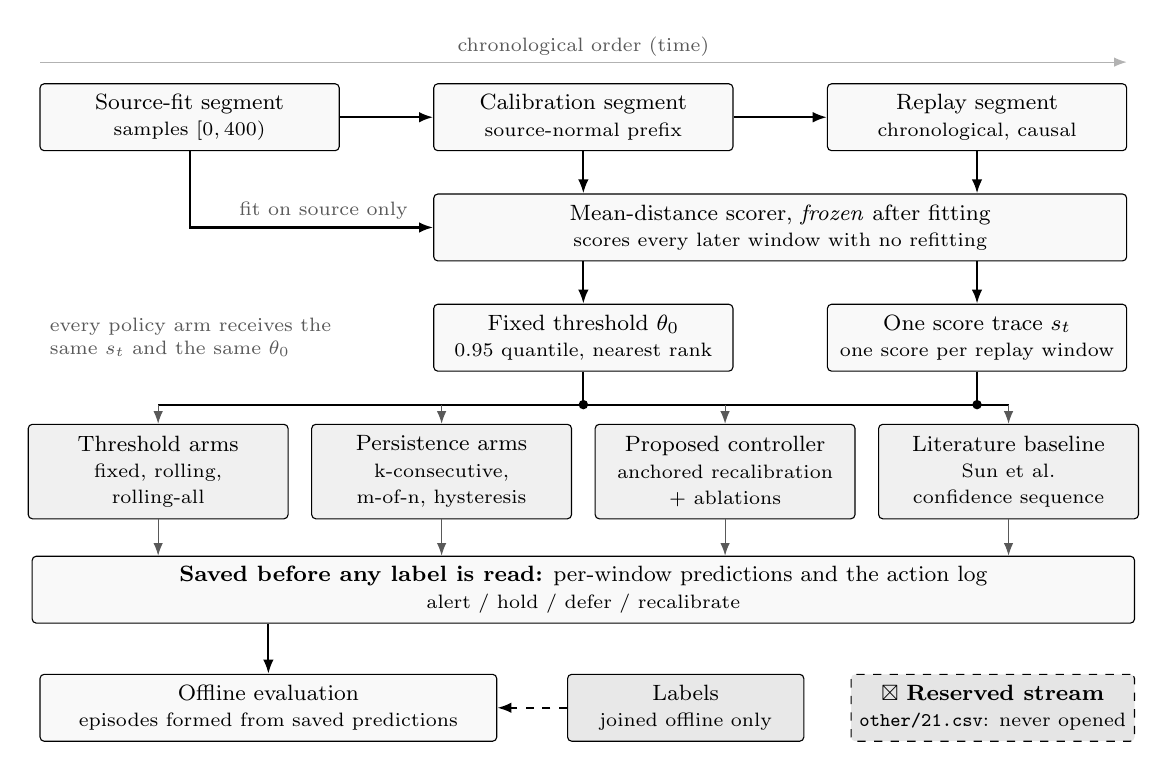
\begin{tikzpicture}[
    x=1mm, y=1mm,
    font=\footnotesize,
    box/.style={draw, rounded corners=1.5pt, align=center, inner sep=2pt,
                fill=gray!5, minimum height=8.5mm},
    arm/.style={box, fill=gray!12, minimum width=33mm, minimum height=12mm},
    flow/.style={-{Latex[length=1.8mm]}, thick},
    feed/.style={-{Latex[length=1.6mm]}, gray!70!black},
    note/.style={gray!70!black, font=\scriptsize, align=left},
]

% --- Row A: one source stream, split in chronological order -------------------
\draw[-{Latex[length=1.6mm]}, gray!60] (-19,7) -- (119,7)
    node[midway, above=-0.5mm, note] {chronological order (time)};
\node[box, minimum width=38mm] (src) at (0,0)
    {Source-fit segment\\\scriptsize samples $[0,400)$};
\node[box, minimum width=38mm] (cal) at (50,0)
    {Calibration segment\\\scriptsize source-normal prefix};
\node[box, minimum width=38mm] (rep) at (100,0)
    {Replay segment\\\scriptsize chronological, causal};
\draw[flow] (src) -- (cal);
\draw[flow] (cal) -- (rep);

% --- Row B: the scorer is fit once, on the source segment only -----------------
\node[box, minimum width=88mm] (scorer) at (75,-14)
    {Mean-distance scorer, \emph{frozen} after fitting\\
     \scriptsize scores every later window with no refitting};
\draw[flow] (src.south) -- (0,-14) -- (scorer.west)
    node[pos=0.55, above=-0.3mm, note] {fit on source only};
\draw[flow] (cal.south) -- (cal.south |- scorer.north);
\draw[flow] (rep.south) -- (rep.south |- scorer.north);

% --- Row C: calibration gives theta_0; replay gives the single score trace -----
\node[box, minimum width=38mm] (thr) at (50,-28)
    {Fixed threshold $\theta_0$\\\scriptsize 0.95 quantile, nearest rank};
\node[box, minimum width=38mm] (trace) at (100,-28)
    {One score trace $s_t$\\\scriptsize one score per replay window};
\draw[flow] (thr.north |- scorer.south) -- (thr.north);
\draw[flow] (trace.north |- scorer.south) -- (trace.north);
\node[note, anchor=west] at (-19,-28)
    {every policy arm receives the\\same $s_t$ and the same $\theta_0$};

% --- Row D: the identical inputs fan out to every policy arm -------------------
\draw[thick] (thr.south) -- (50,-36.5);
\draw[thick] (trace.south) -- (100,-36.5);
\draw[thick] (-4,-36.5) -- (104,-36.5);
\fill (50,-36.5) circle (0.6) (100,-36.5) circle (0.6);
\node[arm] (a1) at (-4,-45)  {Threshold arms\\\scriptsize fixed, rolling,\\\scriptsize rolling-all};
\node[arm] (a2) at (32,-45)  {Persistence arms\\\scriptsize k-consecutive,\\\scriptsize m-of-n, hysteresis};
\node[arm] (a3) at (68,-45)  {Proposed controller\\\scriptsize anchored recalibration\\\scriptsize + ablations};
\node[arm] (a4) at (104,-45) {Literature baseline\\\scriptsize Sun et al.\\\scriptsize confidence sequence};
\foreach \a in {a1,a2,a3,a4} \draw[feed] (\a.north |- 0,-36.5) -- (\a.north);

% --- Row E: outputs saved before any label exists in the process ---------------
\node[box, minimum width=140mm] (saved) at (50,-60)
    {\textbf{Saved before any label is read:} per-window predictions and the action log\\
     \scriptsize alert / hold / defer / recalibrate};
\foreach \a in {a1,a2,a3,a4} \draw[feed] (\a.south) -- (\a.south |- saved.north);

% --- Row F: labels are joined offline only; the reserved stream stays locked ---
\node[box, minimum width=58mm] (eval) at (10,-75)
    {Offline evaluation\\\scriptsize episodes formed from saved predictions};
\node[box, minimum width=30mm, fill=gray!18] (labels) at (63,-75)
    {Labels\\\scriptsize joined offline only};
\draw[flow] (eval.north |- saved.south) -- (eval.north);
\draw[flow, dashed] (labels.west) -- (eval.east);
\node[box, minimum width=36mm, dashed, fill=gray!20] (reserved) at (102,-75)
    {$\boxtimes$\ \textbf{Reserved stream}\\\scriptsize\texttt{other/21.csv}: never opened};

\end{tikzpicture}
}
  \caption{Chronological split and causal data flow. One frozen scorer produces one
  score trace, which every policy arm receives unchanged; outputs are saved before
  labels are joined offline. The reserved stream is never opened.}
  \label{fig:flow}
\end{figure}

\claim{4}{\Simplemented}{We implement recalibration as one guarded action among four.}
The proposed controller (class \texttt{AnchoredRecalibrationPolicy}) keeps a threshold
$\theta$ starting at $\theta_0$, a mode (\textsc{normal}, \textsc{suspect} or
\textsc{escalated}), a defer counter $c$, and a buffer $R$ of the last $L$ scores of
\emph{every} window, so admission never depends on a decision. Listing~\ref{lst:ctrl}
is the frozen rule and Table~\ref{tab:actions} summarises it.

\begin{lstlisting}[style=ctrl, caption={The frozen controller, transcribed exactly from the protocol. \texttt{quantile} is nearest rank; \texttt{median} is the ordinary median.}, label={lst:ctrl}, captionpos=b]
append s to R (drop oldest beyond L)
full     = |R| == L
elevated = full and median(R) > theta
if mode == escalated:
    if elevated: return ALERT if s > theta else HOLD    # stay escalated, no recalibration
    mode = normal                                       # elevation over; fall through
if elevated:
    cand   = quantile(R)
    stable = max(R) <= rho * median(R)
    if stable and cand <= kappa * theta0:
        theta = max(theta0, cand); mode = normal; c = 0 # action RECALIBRATE (up)
        return (ALERT if s > theta else normal), action=RECALIBRATE
    if c < D: c += 1; mode = suspect; return DEFER      # guard failed: withhold
    mode = escalated; c = 0; return ALERT if s > theta else HOLD
# not elevated
if mode == suspect: mode = normal; c = 0
if full and theta > theta0 and quantile(R) < theta:
    theta = max(theta0, quantile(R))                    # action RECALIBRATE (return to anchor)
return ALERT if s > theta else HOLD
\end{lstlisting}

\begin{table}[H]
  \centering
  \caption{When the controller takes each action. ``Sustained rise'' means $R$ is full
  and $\mathrm{med}(R) > \theta$.}
  \label{tab:actions}
  \footnotesize
  \begin{tabular}{@{}p{0.52\linewidth}p{0.42\linewidth}@{}}
    \toprule
    Situation at a window end & Action and mode \\
    \midrule
    No sustained rise & \textsc{hold}, or \textsc{alert} if $s > \theta$; mode normal \\
    Sustained rise, stable ($\max R \le \rho\,\mathrm{med}(R)$) and $q(R) \le \kappa\theta_0$
      & \textsc{recalibrate} to $\max(\theta_0, q(R))$; mode normal \\
    Sustained rise, guard fails, fewer than $D$ deferrals so far & \textsc{defer}; mode suspect \\
    Sustained rise, guard still failing after $D$ deferrals
      & escalate: \textsc{alert} if $s>\theta$ else \textsc{hold}; no recalibration while
      the rise lasts \\
    Rise over, $\theta > \theta_0$ and $q(R) < \theta$ & \textsc{recalibrate} back to
      $\max(\theta_0, q(R))$ \\
    \bottomrule
  \end{tabular}
\end{table}

\paragraph{Parameters were fixed before any outcome was seen.}
$L=10$ and $q=0.95$ are the existing rolling baseline's values, and the defer limit is
$D=L=10$. The cap $\kappa=4$ declares the largest benign rise an operator accepts (four
times $\theta_0$), and the stability bound $\rho=2$ declares that no window in a buffer
may exceed twice its median. Both are operating assumptions, not estimates; on the SKAB
streams the guard is never reached, so no SKAB outcome could have informed them.
Figure~\ref{fig:concept} contrasts the three admission rules schematically.

\begin{figure}[H]
  \centering
  \aifigure{fig-concept}{\resizebox{0.62\linewidth}{!}{% F-concept -- SCHEMATIC (not data) of three admission regimes.
% self-referential ratchets down; unconditional absorbs a sustained fault;
% anchored/separated stays in a bounded band [theta0, kappa*theta0].
% Hand-drawn schematic curves only -- no measured values, no axis numbers.
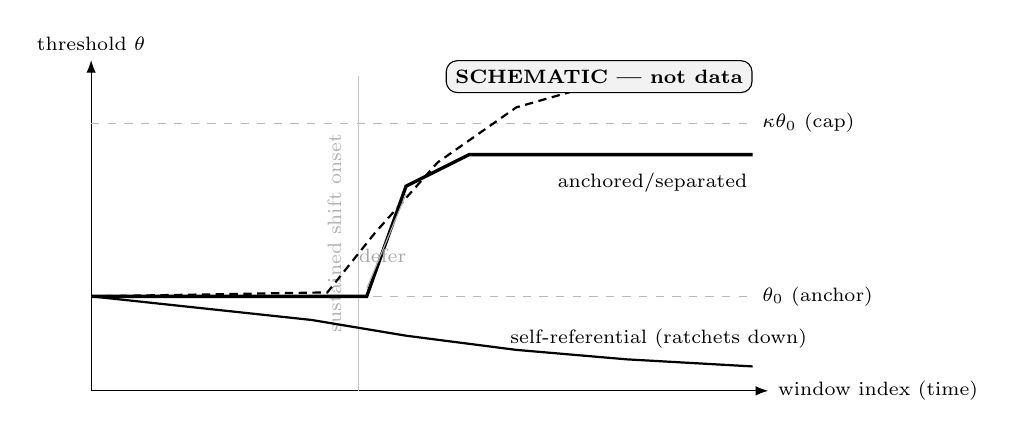
\begin{tikzpicture}[font=\footnotesize, x=1mm, y=1mm]

  % axes
  \draw[-{Latex[length=1.6mm]}] (0,0) -- (86,0) node[right] {\scriptsize window index (time)};
  \draw[-{Latex[length=1.6mm]}] (0,0) -- (0,42) node[above] {\scriptsize threshold $\theta$};

  % anchor and cap reference lines
  \draw[gray!55, dashed] (0,12) -- (84,12) node[right, black] {\scriptsize $\theta_0$ (anchor)};
  \draw[gray!55, dashed] (0,34) -- (84,34) node[right, black] {\scriptsize $\kappa\theta_0$ (cap)};

  % onset of a sustained shift/fault marker
  \draw[gray!45] (34,0) -- (34,40);
  \node[gray!60, rotate=90, anchor=south, font=\scriptsize] at (33,20) {sustained shift onset};

  % (1) self-referential: monotone non-increasing -- ratchets DOWN
  \draw[thick]
    (0,12) -- (14,10.5) -- (28,9) -- (40,7) -- (54,5.2) -- (68,4) -- (84,3.1);
  \node[anchor=west, font=\scriptsize] at (52,6.6) {self-referential (ratchets down)};

  % (2) unconditional: tracks whatever arrives -- absorbs the fault upward, unbounded past cap
  \draw[thick, densely dashed]
    (0,12) -- (30,12.5) -- (36,20) -- (44,29) -- (54,36) -- (68,40) -- (80,41.5);
  \node[anchor=west, font=\scriptsize] at (46,40.5) {unconditional (absorbs fault)};

  % (3) anchored / separated: stays within [theta0, kappa*theta0]
  \draw[very thick]
    (0,12) -- (30,12) -- (35,12) -- (40,26) -- (48,30) -- (60,30) -- (72,30) -- (84,30);
  \node[anchor=west, font=\scriptsize] at (58,26.5) {anchored/separated};
  % small "defer" bracket during the unstable transition
  \draw[gray!60] (35,13) -- (40,25);
  \node[gray!70, font=\scriptsize, anchor=south] at (37,15) {defer};

  % schematic banner
  \node[draw, rounded corners, fill=gray!10, font=\scriptsize\bfseries,
        anchor=north east] at (84,42) {SCHEMATIC --- not data};

\end{tikzpicture}
}}
  \caption{Schematic, not data. Self-referential admission ratchets the threshold down;
  unconditional admission follows a sustained fault up; anchored, separated admission
  stays in $[\theta_0, \kappa\theta_0]$ and defers through an unstable transition.}
  \label{fig:concept}
\end{figure}

\paragraph{Policy arms.}
Table~\ref{tab:arms} lists the eleven arms. The five previously audited arms reproduce
their corrected baseline rows exactly, which serves as a regression gate.

\begin{table}[H]
  \centering
  \caption{Policy arms. Every arm replays the identical score trace of its stream.}
  \label{tab:arms}
  \small
  \begin{tabularx}{\linewidth}{@{}lX@{}}
    \toprule
    Arm & Role\\
    \midrule
    \texttt{fixed\_threshold} & anchor only (existing)\\
    \texttt{rolling\_threshold} (normal-only) & self-referential admission, $L{=}10$, $q{=}0.95$ (existing)\\
    \texttt{rolling\_threshold\_all} & admits every window, no guard (existing)\\
    \texttt{k\_consecutive} ($k{=}3$), \texttt{m\_of\_n} (3/5), \texttt{hysteresis} & persistence and latch rules (existing)\\
    \texttt{anchored\_recalibration} & proposed controller (new)\\
    \texttt{anchored\_no\_cap} / \texttt{no\_stability} / \texttt{no\_defer} & ablations: $\kappa{=}\infty$ / $\rho{=}\infty$ / $D{=}0$\\
    \texttt{sun\_confidence\_sequence} & Sun et al.\ (ICML 2024) Algorithm~1, re-implemented\\
    \bottomrule
  \end{tabularx}
\end{table}

\paragraph{Synthetic stress family.}
Table~\ref{tab:synthetic-family} defines seven deterministic stress cases on a period-16
signal of length 1600 (input \texttt{synthetic\_\allowbreak periodic\_\allowbreak v1}),
using the same windows, scorer, calibration and arms. Offsets apply over half-open
ranges; a spiky fault adds $+6.0$ on alternating 4-sample windows. These cases test the
mechanism; they are not evidence of real-world benefit.

\begin{table}[H]
  \centering
  \caption{Synthetic stress family: what each case adds and what it tests.}
  \label{tab:synthetic-family}
  \small
  \begin{tabularx}{\linewidth}{@{}llX@{}}
    \toprule
    ID & Offsets / fault & Tests\\
    \midrule
    Y1 & $+2.0$ on $[800,1600)$; no event & adapting to a new normal\\
    Y2 & $+0.25$ at each of $800,810,\dots,870$ up to $+2.0$; no event & an unstable transition (defer)\\
    Y3 & Y1 plus a spiky fault on $[1200,1300)$ & catching a fault after adapting\\
    Y4 & $+2.0$ on $[800,1600)$, labelled as an event & the declared limit (H4)\\
    Y5 & spiky fault on $[800,900)$ & onset alert, then the cost of deferring\\
    Y6 & $+5.0$ on $[800,1600)$; no event & the cost of the cap $\kappa$\\
    Y7 & $+2.0$ on $[800,1100)$; spiky fault on $[1300,1400)$ & returning to the anchor\\
    \bottomrule
  \end{tabularx}
\end{table}

\paragraph{Hypotheses.}
Table~\ref{tab:hyp} fixes each hypothesis and the result that would refute it. H2 is a
no-harm check, not a test of benefit: before freezing we saw that no 10-window block of
either SKAB stream has a median above $\theta_0$, so the controller was predicted to act
exactly like the fixed threshold there. Benefit is tested only in H3 and in the next
experiment (Section~\ref{sec:conclusion}).

\begin{table}[H]
  \centering
  \caption{Hypotheses, fixed before the study ran. All tests use common score traces.}
  \label{tab:hyp}
  \small
  \begin{tabularx}{\linewidth}{@{}lXX@{}}
    \toprule
    ID & Hypothesis & Refuted if\\
    \midrule
    H1 & Normal-only rolling recalibration is a one-way ratchet, and its SKAB alert volume is a result of that. & The normal-only rolling threshold ever increases.\\
    H2 & The controller keeps event recall $1/1$ on valve1 and valve2 with false episodes $\le$ fixed (no harm). & Recall $<1/1$ on either stream, or more false episodes than fixed.\\
    H3 & On benign synthetic shifts the controller cuts non-event alert duration versus fixed and normal-only rolling, and still alerts on spiky faults after a shift. & No cut on Y1/Y2, or the Y3/Y7 faults are missed.\\
    H4 & No label-free rule can separate a benign shift from a fault of identical shape, so the controller absorbs Y4 after onset. & Declared limit: reported either way, not a refutation target.\\
    \bottomrule
  \end{tabularx}
\end{table}

% Guideline item 8: Simulation Platform and Requirements.
\section{Simulation Platform and Requirements}\label{sec:platform}

\paragraph{Software.}
The platform is a Python 3.12 package that uses only the standard library, with
\texttt{unittest} for its tests. It provides reusable loaders, chronological splits, a
scoring interface, fixed-quantile calibration, the policy arms and an offline
evaluator. Runs save per-window predictions and an action log, and every reported row
is recomputed by an independent script (\texttt{recompute\_evaluations.py}) before it
enters this report. Execution is deterministic: scoring and policies use no randomness,
and the one randomized property test seeds its own generator. No GPU is needed; each
run records its elapsed time and peak Python memory as its resource scope. The report
and its figures build with a basic \TeX\ Live 2026 installation.

\paragraph{Data.}\Smeasured{}
The development data are two SKAB streams, \texttt{valve1/0.csv} and
\texttt{valve2/0.csv}~\citep{skab2020}, scored on the single \texttt{Current} channel.
Each contains exactly one labelled event (valve1 $[574,975)$, valve2 $[562,956)$), so
recall is measured over one event per stream. Origin and licence are not independently
verified (valve1's acquisition URL is unknown; valve2's provenance comes from an earlier
manifest), so all results are development-only. The stream
\texttt{SKAB/other/21.csv} is named as reserved in the manifest, but the authority and
recipe for that reservation are disputed; it was never opened and no claim rests on it.

% Results and Analysis, organised by claim (C1-C6 from page 2).
\section{Results and Analysis}\label{sec:results}

All numbers come from the saved study \texttt{20260929-policy-study-v2}, which an
independent script recomputes with zero mismatches over 99 runs. Within a stream every
arm replays a byte-identical score trace, so differences come from decision rules alone.
Durations and delays are in sample-index units.

\subsection{The ratchet and its cost (C1, C2; H1)}\label{sec:results-ratchet}
\claim{1}{\Sproved\,\Smeasured}{We prove the ratchet and observe it in the saved
traces.}
The normal-only rolling threshold records 0 increases in 143 (valve1) and 140 (valve2)
replay steps. It falls from $1.309$ to $0.258$ on valve1 and from $1.126$ to $0.406$ on
valve2, below the median replay score (Figure~\ref{fig:ratchet}), exactly as
Proposition~\ref{prop:ratchet} predicts.

\claim{2}{\Smeasured}{We measure what the ratchet costs.}
Rolling (normal-only) detects the same single event as the fixed threshold, but with
$16.2\times$ the alert windows on valve1 (97 vs 6) and $3.9\times$ on valve2 (70 vs 18)
(Table~\ref{tab:baseline}). The extra alerts come from the falling threshold, not from
extra anomalies.

\begin{figure}[tbp]
  \centering
  \resizebox{0.9\linewidth}{!}{\providecolor{scblack}{RGB}{0,0,0}%
\providecolor{scblue}{RGB}{31,78,150}%
\providecolor{scred}{RGB}{170,40,30}%
\providecolor{scgreen}{RGB}{20,110,60}%
\providecolor{scgray}{RGB}{120,120,120}%
\providecolor{scevent}{RGB}{60,60,60}%
\begin{tikzpicture}[>=stealth,line join=round,line cap=round]
  \begin{scope}[xshift=0.00cm]
  \fill[scevent,opacity=0.14] (0.000,0) rectangle (3.994,4.300);
  \draw[scgray,solid,line width=0.5pt] (0.000,0.848) -- (0.040,0.765) -- (0.080,1.440) -- (0.120,1.425) -- (0.161,0.820) -- (0.201,0.883) -- (0.241,0.554) -- (0.281,0.497) -- (0.321,0.000) -- (0.361,1.159) -- (0.401,1.355) -- (0.442,1.179) -- (0.482,1.299) -- (0.522,1.356) -- (0.562,1.068) -- (0.602,0.000) -- (0.642,0.482) -- (0.682,0.915) -- (0.723,0.991) -- (0.763,0.926) -- (0.803,0.821) -- (0.843,1.407) -- (0.883,1.062) -- (0.923,0.870) -- (0.963,0.887) -- (1.004,0.094) -- (1.044,0.771) -- (1.084,0.894) -- (1.124,0.275) -- (1.164,0.554) -- (1.204,1.098) -- (1.244,0.000) -- (1.285,0.140) -- (1.325,0.954) -- (1.365,1.237) -- (1.405,0.955) -- (1.445,1.132) -- (1.485,0.928) -- (1.525,0.000) -- (1.565,0.659) -- (1.606,4.099) -- (1.646,0.746) -- (1.686,1.094) -- (1.726,1.048) -- (1.766,0.996) -- (1.806,0.869) -- (1.846,0.994) -- (1.887,1.458) -- (1.927,4.106) -- (1.967,0.637) -- (2.007,1.186) -- (2.047,1.118) -- (2.087,0.949) -- (2.127,0.000) -- (2.168,0.180) -- (2.208,0.647) -- (2.248,1.011) -- (2.288,1.216) -- (2.328,1.161) -- (2.368,0.925) -- (2.408,0.920) -- (2.449,1.271) -- (2.489,1.138) -- (2.529,0.830) -- (2.569,0.983) -- (2.609,0.000) -- (2.649,0.768) -- (2.689,1.203) -- (2.730,0.985) -- (2.770,0.880) -- (2.810,1.358) -- (2.850,0.904) -- (2.890,0.691) -- (2.930,0.925) -- (2.970,0.174) -- (3.011,0.859) -- (3.051,0.856) -- (3.091,0.780) -- (3.131,1.020) -- (3.171,1.278) -- (3.211,0.781) -- (3.251,1.260) -- (3.292,1.191) -- (3.332,1.107) -- (3.372,0.322) -- (3.412,0.000) -- (3.452,0.927) -- (3.492,1.057) -- (3.532,0.000) -- (3.573,0.926) -- (3.613,0.965) -- (3.653,1.187) -- (3.693,1.000) -- (3.733,0.973) -- (3.773,1.106) -- (3.813,0.714) -- (3.854,0.348) -- (3.894,1.093) -- (3.934,0.567) -- (3.974,1.338) -- (4.014,1.104) -- (4.054,1.157) -- (4.094,1.073) -- (4.135,0.977) -- (4.175,1.261) -- (4.215,0.469) -- (4.255,0.820) -- (4.295,0.269) -- (4.335,0.991) -- (4.375,0.253) -- (4.415,0.514) -- (4.456,1.133) -- (4.496,0.000) -- (4.536,1.042) -- (4.576,0.976) -- (4.616,1.114) -- (4.656,0.286) -- (4.696,0.349) -- (4.737,0.322) -- (4.777,0.432) -- (4.817,0.963) -- (4.857,0.314) -- (4.897,1.232) -- (4.937,0.805) -- (4.977,1.088) -- (5.018,1.137) -- (5.058,0.749) -- (5.098,0.577) -- (5.138,0.496) -- (5.178,0.509) -- (5.218,1.313) -- (5.258,1.111) -- (5.299,0.454) -- (5.339,0.000) -- (5.379,0.305) -- (5.419,0.000) -- (5.459,0.877) -- (5.499,0.638) -- (5.539,1.271) -- (5.580,1.279) -- (5.620,1.147) -- (5.660,1.103) -- (5.700,1.025);
  \draw[scblack,solid,line width=0.8pt] (0,1.381) -- (5.700,1.381);
  \draw[scred,dashed,line width=0.8pt] (0.000,1.381) -- (0.040,0.848) -- (0.080,0.848) -- (0.120,0.848) -- (0.161,0.848) -- (0.201,0.848) -- (0.241,0.848) -- (0.281,0.848) -- (0.321,0.848) -- (0.361,0.848) -- (0.401,0.848) -- (0.442,0.848) -- (0.482,0.848) -- (0.522,0.848) -- (0.562,0.848) -- (0.602,0.848) -- (0.642,0.848) -- (0.682,0.848) -- (0.723,0.848) -- (0.763,0.848) -- (0.803,0.848) -- (0.843,0.848) -- (0.883,0.848) -- (0.923,0.848) -- (0.963,0.848) -- (1.004,0.848) -- (1.044,0.848) -- (1.084,0.821) -- (1.124,0.821) -- (1.164,0.821) -- (1.204,0.821) -- (1.244,0.821) -- (1.285,0.821) -- (1.325,0.821) -- (1.365,0.821) -- (1.405,0.821) -- (1.445,0.821) -- (1.485,0.821) -- (1.525,0.821) -- (1.565,0.821) -- (1.606,0.821) -- (1.646,0.821) -- (1.686,0.821) -- (1.726,0.821) -- (1.766,0.821) -- (1.806,0.821) -- (1.846,0.821) -- (1.887,0.821) -- (1.927,0.821) -- (1.967,0.821) -- (2.007,0.771) -- (2.047,0.771) -- (2.087,0.771) -- (2.127,0.771) -- (2.168,0.771) -- (2.208,0.746) -- (2.248,0.746) -- (2.288,0.746) -- (2.328,0.746) -- (2.368,0.746) -- (2.408,0.746) -- (2.449,0.746) -- (2.489,0.746) -- (2.529,0.746) -- (2.569,0.746) -- (2.609,0.746) -- (2.649,0.746) -- (2.689,0.746) -- (2.730,0.746) -- (2.770,0.746) -- (2.810,0.746) -- (2.850,0.746) -- (2.890,0.746) -- (2.930,0.746) -- (2.970,0.746) -- (3.011,0.746) -- (3.051,0.746) -- (3.091,0.746) -- (3.131,0.746) -- (3.171,0.746) -- (3.211,0.746) -- (3.251,0.746) -- (3.292,0.746) -- (3.332,0.746) -- (3.372,0.746) -- (3.412,0.746) -- (3.452,0.746) -- (3.492,0.746) -- (3.532,0.746) -- (3.573,0.691) -- (3.613,0.691) -- (3.653,0.691) -- (3.693,0.691) -- (3.733,0.691) -- (3.773,0.691) -- (3.813,0.691) -- (3.854,0.691) -- (3.894,0.691) -- (3.934,0.691) -- (3.974,0.691) -- (4.014,0.691) -- (4.054,0.691) -- (4.094,0.691) -- (4.135,0.691) -- (4.175,0.691) -- (4.215,0.691) -- (4.255,0.691) -- (4.295,0.691) -- (4.335,0.691) -- (4.375,0.691) -- (4.415,0.691) -- (4.456,0.567) -- (4.496,0.567) -- (4.536,0.567) -- (4.576,0.567) -- (4.616,0.567) -- (4.656,0.567) -- (4.696,0.567) -- (4.737,0.567) -- (4.777,0.567) -- (4.817,0.567) -- (4.857,0.567) -- (4.897,0.514) -- (4.937,0.514) -- (4.977,0.514) -- (5.018,0.514) -- (5.058,0.514) -- (5.098,0.514) -- (5.138,0.514) -- (5.178,0.514) -- (5.218,0.514) -- (5.258,0.514) -- (5.299,0.514) -- (5.339,0.514) -- (5.379,0.509) -- (5.419,0.509) -- (5.459,0.509) -- (5.499,0.509) -- (5.539,0.509) -- (5.580,0.509) -- (5.620,0.509) -- (5.660,0.509) -- (5.700,0.509);
  \draw[scblue,dotted,line width=0.8pt] (0.000,1.381) -- (0.040,0.848) -- (0.080,0.848) -- (0.120,1.440) -- (0.161,1.440) -- (0.201,1.440) -- (0.241,1.440) -- (0.281,1.440) -- (0.321,1.440) -- (0.361,1.440) -- (0.401,1.440) -- (0.442,1.440) -- (0.482,1.440) -- (0.522,1.425) -- (0.562,1.356) -- (0.602,1.356) -- (0.642,1.356) -- (0.682,1.356) -- (0.723,1.356) -- (0.763,1.356) -- (0.803,1.356) -- (0.843,1.356) -- (0.883,1.407) -- (0.923,1.407) -- (0.963,1.407) -- (1.004,1.407) -- (1.044,1.407) -- (1.084,1.407) -- (1.124,1.407) -- (1.164,1.407) -- (1.204,1.407) -- (1.244,1.407) -- (1.285,1.098) -- (1.325,1.098) -- (1.365,1.098) -- (1.405,1.237) -- (1.445,1.237) -- (1.485,1.237) -- (1.525,1.237) -- (1.565,1.237) -- (1.606,1.237) -- (1.646,4.099) -- (1.686,4.099) -- (1.726,4.099) -- (1.766,4.099) -- (1.806,4.099) -- (1.846,4.099) -- (1.887,4.099) -- (1.927,4.099) -- (1.967,4.106) -- (2.007,4.106) -- (2.047,4.106) -- (2.087,4.106) -- (2.127,4.106) -- (2.168,4.106) -- (2.208,4.106) -- (2.248,4.106) -- (2.288,4.106) -- (2.328,4.106) -- (2.368,1.216) -- (2.408,1.216) -- (2.449,1.216) -- (2.489,1.271) -- (2.529,1.271) -- (2.569,1.271) -- (2.609,1.271) -- (2.649,1.271) -- (2.689,1.271) -- (2.730,1.271) -- (2.770,1.271) -- (2.810,1.271) -- (2.850,1.358) -- (2.890,1.358) -- (2.930,1.358) -- (2.970,1.358) -- (3.011,1.358) -- (3.051,1.358) -- (3.091,1.358) -- (3.131,1.358) -- (3.171,1.358) -- (3.211,1.358) -- (3.251,1.278) -- (3.292,1.278) -- (3.332,1.278) -- (3.372,1.278) -- (3.412,1.278) -- (3.452,1.278) -- (3.492,1.278) -- (3.532,1.278) -- (3.573,1.278) -- (3.613,1.260) -- (3.653,1.260) -- (3.693,1.191) -- (3.733,1.187) -- (3.773,1.187) -- (3.813,1.187) -- (3.854,1.187) -- (3.894,1.187) -- (3.934,1.187) -- (3.974,1.187) -- (4.014,1.338) -- (4.054,1.338) -- (4.094,1.338) -- (4.135,1.338) -- (4.175,1.338) -- (4.215,1.338) -- (4.255,1.338) -- (4.295,1.338) -- (4.335,1.338) -- (4.375,1.338) -- (4.415,1.261) -- (4.456,1.261) -- (4.496,1.261) -- (4.536,1.261) -- (4.576,1.261) -- (4.616,1.133) -- (4.656,1.133) -- (4.696,1.133) -- (4.737,1.133) -- (4.777,1.133) -- (4.817,1.133) -- (4.857,1.133) -- (4.897,1.114) -- (4.937,1.232) -- (4.977,1.232) -- (5.018,1.232) -- (5.058,1.232) -- (5.098,1.232) -- (5.138,1.232) -- (5.178,1.232) -- (5.218,1.232) -- (5.258,1.313) -- (5.299,1.313) -- (5.339,1.313) -- (5.379,1.313) -- (5.419,1.313) -- (5.459,1.313) -- (5.499,1.313) -- (5.539,1.313) -- (5.580,1.313) -- (5.620,1.313) -- (5.660,1.279) -- (5.700,1.279);
  \node[font=\scriptsize,scred,anchor=north west,fill=white,fill opacity=0.9,text opacity=1,inner sep=1pt,align=left] at (0.12,4.220) {start 1.309\\end 0.258};
  \draw[scblack] (0,0) rectangle (5.700,4.300);
  \draw[scblack] (0.000,0) -- (0.000,-0.08);
  \node[font=\scriptsize,below] at (0.000,-0.08) {577};
  \draw[scblack] (2.850,0) -- (2.850,-0.08);
  \node[font=\scriptsize,below] at (2.850,-0.08) {861};
  \draw[scblack] (5.700,0) -- (5.700,-0.08);
  \node[font=\scriptsize,below] at (5.700,-0.08) {1145};
  \draw[scblack] (0,0.000) -- (-0.08,0.000);
  \node[font=\scriptsize,left] at (-0.10,0.000) {$10^{-1}$};
  \draw[scblack] (0,1.237) -- (-0.08,1.237);
  \node[font=\scriptsize,left] at (-0.10,1.237) {$10^{0}$};
  \draw[scblack] (0,2.473) -- (-0.08,2.473);
  \node[font=\scriptsize,left] at (-0.10,2.473) {$10^{1}$};
  \draw[scblack] (0,3.710) -- (-0.08,3.710);
  \node[font=\scriptsize,left] at (-0.10,3.710) {$10^{2}$};
  \node[font=\scriptsize,below=0.42cm] at (2.850,0) {sample index (window end)};
  \node[font=\scriptsize,rotate=90] at (-0.920,2.150) {replay score};
  \node[font={\scriptsize\bfseries},above] at (2.850,4.340) {valve1 (score, log$_{10}$)};
  \end{scope}
  \begin{scope}[xshift=7.20cm]
  \fill[scevent,opacity=0.14] (0.000,0) rectangle (4.008,4.300);
  \draw[scgray,solid,line width=0.5pt] (0.000,1.239) -- (0.041,0.279) -- (0.082,0.156) -- (0.123,4.122) -- (0.164,1.366) -- (0.205,1.245) -- (0.246,1.404) -- (0.287,0.981) -- (0.328,1.277) -- (0.369,0.000) -- (0.410,1.164) -- (0.451,0.476) -- (0.492,0.661) -- (0.533,1.250) -- (0.574,1.072) -- (0.615,1.190) -- (0.656,0.972) -- (0.697,1.246) -- (0.738,0.516) -- (0.779,0.952) -- (0.820,0.000) -- (0.861,1.204) -- (0.902,0.000) -- (0.943,0.601) -- (0.984,0.302) -- (1.025,1.409) -- (1.066,1.210) -- (1.107,1.369) -- (1.148,0.996) -- (1.189,1.015) -- (1.230,1.104) -- (1.271,0.720) -- (1.312,0.266) -- (1.353,0.000) -- (1.394,0.488) -- (1.435,1.153) -- (1.476,1.093) -- (1.517,4.063) -- (1.558,1.453) -- (1.599,1.075) -- (1.640,0.000) -- (1.681,0.911) -- (1.722,0.786) -- (1.763,1.128) -- (1.804,0.884) -- (1.845,0.667) -- (1.886,1.217) -- (1.927,0.701) -- (1.968,0.988) -- (2.009,0.908) -- (2.050,1.034) -- (2.091,1.404) -- (2.132,1.347) -- (2.173,1.168) -- (2.214,0.971) -- (2.255,1.105) -- (2.296,0.000) -- (2.337,0.637) -- (2.378,0.923) -- (2.419,0.821) -- (2.460,0.887) -- (2.501,0.416) -- (2.542,0.654) -- (2.583,1.084) -- (2.624,1.043) -- (2.665,1.102) -- (2.706,1.075) -- (2.747,0.912) -- (2.788,1.335) -- (2.829,0.496) -- (2.871,0.000) -- (2.912,1.025) -- (2.953,1.184) -- (2.994,0.836) -- (3.035,0.815) -- (3.076,1.135) -- (3.117,1.256) -- (3.158,1.070) -- (3.199,0.840) -- (3.240,1.269) -- (3.281,1.210) -- (3.322,1.286) -- (3.363,0.909) -- (3.404,1.283) -- (3.445,1.221) -- (3.486,1.023) -- (3.527,1.081) -- (3.568,0.400) -- (3.609,0.760) -- (3.650,1.296) -- (3.691,1.205) -- (3.732,0.748) -- (3.773,1.185) -- (3.814,1.398) -- (3.855,1.320) -- (3.896,1.186) -- (3.937,1.446) -- (3.978,0.766) -- (4.019,0.926) -- (4.060,0.000) -- (4.101,0.676) -- (4.142,0.000) -- (4.183,0.412) -- (4.224,0.204) -- (4.265,0.706) -- (4.306,0.904) -- (4.347,1.080) -- (4.388,0.899) -- (4.429,1.279) -- (4.470,1.259) -- (4.511,0.254) -- (4.552,1.060) -- (4.593,1.076) -- (4.634,0.135) -- (4.675,0.792) -- (4.716,1.035) -- (4.757,1.246) -- (4.798,1.489) -- (4.839,4.146) -- (4.880,1.168) -- (4.921,1.355) -- (4.962,0.753) -- (5.003,1.222) -- (5.044,1.118) -- (5.085,0.137) -- (5.126,0.933) -- (5.167,0.274) -- (5.208,1.465) -- (5.249,1.301) -- (5.290,0.989) -- (5.331,0.745) -- (5.372,0.530) -- (5.413,1.027) -- (5.454,0.728) -- (5.495,0.000) -- (5.536,1.227) -- (5.577,1.270) -- (5.618,1.233) -- (5.659,1.182) -- (5.700,0.734);
  \draw[scblack,solid,line width=0.8pt] (0,1.300) -- (5.700,1.300);
  \draw[scred,dashed,line width=0.8pt] (0.000,1.300) -- (0.041,1.239) -- (0.082,1.239) -- (0.123,1.239) -- (0.164,1.239) -- (0.205,1.239) -- (0.246,1.239) -- (0.287,1.239) -- (0.328,1.239) -- (0.369,1.239) -- (0.410,1.239) -- (0.451,1.239) -- (0.492,1.239) -- (0.533,1.239) -- (0.574,1.239) -- (0.615,1.239) -- (0.656,1.239) -- (0.697,1.190) -- (0.738,1.190) -- (0.779,1.190) -- (0.820,1.190) -- (0.861,1.190) -- (0.902,1.190) -- (0.943,1.190) -- (0.984,1.190) -- (1.025,1.190) -- (1.066,1.190) -- (1.107,1.190) -- (1.148,1.190) -- (1.189,1.190) -- (1.230,1.190) -- (1.271,1.104) -- (1.312,1.104) -- (1.353,1.104) -- (1.394,1.104) -- (1.435,1.104) -- (1.476,1.104) -- (1.517,1.104) -- (1.558,1.104) -- (1.599,1.104) -- (1.640,1.104) -- (1.681,1.104) -- (1.722,1.104) -- (1.763,1.104) -- (1.804,1.104) -- (1.845,1.093) -- (1.886,1.093) -- (1.927,1.093) -- (1.968,1.093) -- (2.009,1.093) -- (2.050,1.093) -- (2.091,1.075) -- (2.132,1.075) -- (2.173,1.075) -- (2.214,1.075) -- (2.255,1.034) -- (2.296,1.034) -- (2.337,1.034) -- (2.378,1.034) -- (2.419,1.034) -- (2.460,1.034) -- (2.501,1.034) -- (2.542,1.034) -- (2.583,1.034) -- (2.624,1.034) -- (2.665,1.034) -- (2.706,1.034) -- (2.747,1.034) -- (2.788,1.034) -- (2.829,1.034) -- (2.871,0.971) -- (2.912,0.923) -- (2.953,0.923) -- (2.994,0.923) -- (3.035,0.923) -- (3.076,0.923) -- (3.117,0.923) -- (3.158,0.923) -- (3.199,0.923) -- (3.240,0.912) -- (3.281,0.912) -- (3.322,0.912) -- (3.363,0.912) -- (3.404,0.912) -- (3.445,0.912) -- (3.486,0.912) -- (3.527,0.912) -- (3.568,0.912) -- (3.609,0.912) -- (3.650,0.912) -- (3.691,0.912) -- (3.732,0.912) -- (3.773,0.912) -- (3.814,0.912) -- (3.855,0.912) -- (3.896,0.912) -- (3.937,0.912) -- (3.978,0.912) -- (4.019,0.909) -- (4.060,0.909) -- (4.101,0.909) -- (4.142,0.909) -- (4.183,0.909) -- (4.224,0.909) -- (4.265,0.909) -- (4.306,0.766) -- (4.347,0.766) -- (4.388,0.766) -- (4.429,0.766) -- (4.470,0.766) -- (4.511,0.766) -- (4.552,0.766) -- (4.593,0.766) -- (4.634,0.766) -- (4.675,0.766) -- (4.716,0.766) -- (4.757,0.766) -- (4.798,0.766) -- (4.839,0.766) -- (4.880,0.766) -- (4.921,0.766) -- (4.962,0.766) -- (5.003,0.766) -- (5.044,0.766) -- (5.085,0.766) -- (5.126,0.753) -- (5.167,0.753) -- (5.208,0.753) -- (5.249,0.753) -- (5.290,0.753) -- (5.331,0.753) -- (5.372,0.753) -- (5.413,0.753) -- (5.454,0.753) -- (5.495,0.753) -- (5.536,0.753) -- (5.577,0.753) -- (5.618,0.753) -- (5.659,0.753) -- (5.700,0.753);
  \draw[scblue,dotted,line width=0.8pt] (0.000,1.300) -- (0.041,1.239) -- (0.082,1.239) -- (0.123,1.239) -- (0.164,4.122) -- (0.205,4.122) -- (0.246,4.122) -- (0.287,4.122) -- (0.328,4.122) -- (0.369,4.122) -- (0.410,4.122) -- (0.451,4.122) -- (0.492,4.122) -- (0.533,4.122) -- (0.574,1.404) -- (0.615,1.404) -- (0.656,1.404) -- (0.697,1.277) -- (0.738,1.277) -- (0.779,1.250) -- (0.820,1.250) -- (0.861,1.250) -- (0.902,1.250) -- (0.943,1.250) -- (0.984,1.246) -- (1.025,1.246) -- (1.066,1.409) -- (1.107,1.409) -- (1.148,1.409) -- (1.189,1.409) -- (1.230,1.409) -- (1.271,1.409) -- (1.312,1.409) -- (1.353,1.409) -- (1.394,1.409) -- (1.435,1.409) -- (1.476,1.369) -- (1.517,1.369) -- (1.558,4.063) -- (1.599,4.063) -- (1.640,4.063) -- (1.681,4.063) -- (1.722,4.063) -- (1.763,4.063) -- (1.804,4.063) -- (1.845,4.063) -- (1.886,4.063) -- (1.927,4.063) -- (1.968,1.453) -- (2.009,1.217) -- (2.050,1.217) -- (2.091,1.217) -- (2.132,1.404) -- (2.173,1.404) -- (2.214,1.404) -- (2.255,1.404) -- (2.296,1.404) -- (2.337,1.404) -- (2.378,1.404) -- (2.419,1.404) -- (2.460,1.404) -- (2.501,1.404) -- (2.542,1.347) -- (2.583,1.168) -- (2.624,1.105) -- (2.665,1.105) -- (2.706,1.102) -- (2.747,1.102) -- (2.788,1.102) -- (2.829,1.335) -- (2.871,1.335) -- (2.912,1.335) -- (2.953,1.335) -- (2.994,1.335) -- (3.035,1.335) -- (3.076,1.335) -- (3.117,1.335) -- (3.158,1.335) -- (3.199,1.335) -- (3.240,1.256) -- (3.281,1.269) -- (3.322,1.269) -- (3.363,1.286) -- (3.404,1.286) -- (3.445,1.286) -- (3.486,1.286) -- (3.527,1.286) -- (3.568,1.286) -- (3.609,1.286) -- (3.650,1.286) -- (3.691,1.296) -- (3.732,1.296) -- (3.773,1.296) -- (3.814,1.296) -- (3.855,1.398) -- (3.896,1.398) -- (3.937,1.398) -- (3.978,1.446) -- (4.019,1.446) -- (4.060,1.446) -- (4.101,1.446) -- (4.142,1.446) -- (4.183,1.446) -- (4.224,1.446) -- (4.265,1.446) -- (4.306,1.446) -- (4.347,1.446) -- (4.388,1.080) -- (4.429,1.080) -- (4.470,1.279) -- (4.511,1.279) -- (4.552,1.279) -- (4.593,1.279) -- (4.634,1.279) -- (4.675,1.279) -- (4.716,1.279) -- (4.757,1.279) -- (4.798,1.279) -- (4.839,1.489) -- (4.880,4.146) -- (4.921,4.146) -- (4.962,4.146) -- (5.003,4.146) -- (5.044,4.146) -- (5.085,4.146) -- (5.126,4.146) -- (5.167,4.146) -- (5.208,4.146) -- (5.249,4.146) -- (5.290,1.465) -- (5.331,1.465) -- (5.372,1.465) -- (5.413,1.465) -- (5.454,1.465) -- (5.495,1.465) -- (5.536,1.465) -- (5.577,1.465) -- (5.618,1.465) -- (5.659,1.301) -- (5.700,1.270);
  \node[font=\scriptsize,scred,anchor=north west,fill=white,fill opacity=0.9,text opacity=1,inner sep=1pt,align=left] at (0.12,4.220) {start 1.126\\end 0.406};
  \draw[scblack] (0,0) rectangle (5.700,4.300);
  \draw[scblack] (0.000,0) -- (0.000,-0.08);
  \node[font=\scriptsize,below] at (0.000,-0.08) {565};
  \draw[scblack] (2.850,0) -- (2.850,-0.08);
  \node[font=\scriptsize,below] at (2.850,-0.08) {843};
  \draw[scblack] (5.700,0) -- (5.700,-0.08);
  \node[font=\scriptsize,below] at (5.700,-0.08) {1121};
  \draw[scblack] (0,0.000) -- (-0.08,0.000);
  \node[font=\scriptsize,left] at (-0.10,0.000) {$10^{-1}$};
  \draw[scblack] (0,1.237) -- (-0.08,1.237);
  \node[font=\scriptsize,left] at (-0.10,1.237) {$10^{0}$};
  \draw[scblack] (0,2.473) -- (-0.08,2.473);
  \node[font=\scriptsize,left] at (-0.10,2.473) {$10^{1}$};
  \draw[scblack] (0,3.710) -- (-0.08,3.710);
  \node[font=\scriptsize,left] at (-0.10,3.710) {$10^{2}$};
  \node[font=\scriptsize,below=0.42cm] at (2.850,0) {sample index (window end)};
  \node[font=\scriptsize,rotate=90] at (-0.920,2.150) {replay score};
  \node[font={\scriptsize\bfseries},above] at (2.850,4.340) {valve2 (score, log$_{10}$)};
  \end{scope}
  \draw[scgray,solid,line width=0.9pt] (0.000,-1.150) -- (0.500,-1.150);
  \node[font=\scriptsize,right] at (0.550,-1.150) {replay score};
  \draw[scblack,solid,line width=0.9pt] (2.600,-1.150) -- (3.100,-1.150);
  \node[font=\scriptsize,right] at (3.150,-1.150) {fixed $\theta_0$};
  \draw[scred,dashed,line width=0.9pt] (4.700,-1.150) -- (5.200,-1.150);
  \node[font=\scriptsize,right] at (5.250,-1.150) {rolling (normal-only)};
  \draw[scblue,dotted,line width=0.9pt] (8.600,-1.150) -- (9.100,-1.150);
  \node[font=\scriptsize,right] at (9.150,-1.150) {rolling (all)};
  \fill[scevent,opacity=0.14] (11.500,-1.270) rectangle (12.000,-1.030);
  \node[font=\scriptsize,right] at (12.050,-1.150) {labelled event span};
\end{tikzpicture}%
}
  \caption{Replay score (grey, $\log_{10}$) on valve1 (left) and valve2 (right), with
  the fixed threshold $\theta_0$ (black), the normal-only rolling threshold (red dashed)
  and the admit-all rolling threshold (blue dotted); the labelled event is shaded. Start
  and end threshold values are printed inside each panel. The normal-only threshold only
  ever falls.}
  \label{fig:ratchet}
\end{figure}

\subsection{The scorer, not the policy, limits detection (C3)}\label{sec:results-scorer}
\claim{3}{\Smeasured}{We measure that no alert rule can recover what the scorer does
not separate.}
Inside the labelled event only $6/100$ (valve1) and $13/98$ (valve2) replay windows
exceed $\theta_0$, and the longest run above it is 2 windows on both streams
(Figure~\ref{fig:scorer-limit}). Persistence rules therefore fall short of their own
requirement: \texttt{k\_consecutive} ($k=3$) misses both events and \texttt{m\_of\_n}
(3/5) misses valve1. Each event also covers about 70\% of the replay decisions, so a
single alert anywhere inside it scores full recall. On SKAB, recall of $1/1$ carries
little information; workload, false episodes and the in-event alerted fraction carry it.

\begin{figure}[tbp]
  \centering
  \resizebox{0.88\linewidth}{!}{\definecolor{scblack}{RGB}{ 25, 32, 56}%
\definecolor{scblue}{RGB}{  0,114,178}%
\definecolor{scred}{RGB}{ 213, 94,  0}%
\definecolor{scgreen}{RGB}{  0,158,115}%
\definecolor{scgray}{RGB}{ 88,108,140}%
\definecolor{scevent}{RGB}{230,159,  0}%
\begin{tikzpicture}[>=stealth,line join=round,line cap=round]
  \begin{scope}[xshift=0.00cm]
  \draw[scblack,densely dotted,line width=0.9pt] (0,1.200) -- (5.900,1.200);
  \draw[scblue,dotted,line width=0.8pt] (0.069,0.025) -- (0.206,0.052) -- (0.343,0.062) -- (0.480,0.147) -- (0.617,0.151) -- (0.755,0.156) -- (0.892,0.162) -- (1.029,0.165) -- (1.166,0.167) -- (1.303,0.176) -- (1.441,0.205) -- (1.578,0.214) -- (1.715,0.220) -- (1.852,0.231) -- (1.990,0.237) -- (2.127,0.239) -- (2.264,0.268) -- (2.401,0.301) -- (2.538,0.370) -- (2.676,0.411) -- (2.813,0.422) -- (2.950,0.470) -- (3.087,0.551) -- (3.224,0.564) -- (3.362,0.565) -- (3.499,0.580) -- (3.636,0.619) -- (3.773,0.638) -- (3.910,0.677) -- (4.048,0.696) -- (4.185,0.716) -- (4.322,0.717) -- (4.459,0.726) -- (4.597,0.730) -- (4.734,0.756) -- (4.871,0.761) -- (5.008,0.775) -- (5.145,0.790) -- (5.283,0.908) -- (5.420,0.960) -- (5.557,0.978) -- (5.694,0.991) -- (5.831,1.057);
  \draw[scred,solid,line width=1.0pt] (0.030,0.003) -- (0.088,0.015) -- (0.148,0.026) -- (0.207,0.028) -- (0.266,0.032) -- (0.325,0.051) -- (0.384,0.068) -- (0.443,0.080) -- (0.502,0.109) -- (0.560,0.119) -- (0.620,0.127) -- (0.679,0.128) -- (0.738,0.153) -- (0.797,0.167) -- (0.856,0.175) -- (0.915,0.225) -- (0.974,0.231) -- (1.032,0.257) -- (1.092,0.257) -- (1.151,0.264) -- (1.210,0.300) -- (1.268,0.306) -- (1.328,0.313) -- (1.387,0.332) -- (1.446,0.346) -- (1.505,0.368) -- (1.564,0.381) -- (1.623,0.383) -- (1.681,0.386) -- (1.740,0.392) -- (1.800,0.393) -- (1.859,0.422) -- (1.918,0.423) -- (1.977,0.430) -- (2.035,0.445) -- (2.095,0.452) -- (2.154,0.454) -- (2.213,0.463) -- (2.272,0.463) -- (2.331,0.472) -- (2.390,0.475) -- (2.449,0.479) -- (2.508,0.484) -- (2.567,0.493) -- (2.626,0.504) -- (2.685,0.508) -- (2.744,0.513) -- (2.803,0.513) -- (2.861,0.514) -- (2.921,0.514) -- (2.980,0.515) -- (3.039,0.516) -- (3.098,0.537) -- (3.157,0.542) -- (3.216,0.543) -- (3.275,0.553) -- (3.333,0.562) -- (3.393,0.572) -- (3.451,0.574) -- (3.510,0.580) -- (3.570,0.584) -- (3.629,0.585) -- (3.688,0.590) -- (3.747,0.602) -- (3.806,0.613) -- (3.865,0.645) -- (3.924,0.657) -- (3.983,0.663) -- (4.042,0.670) -- (4.101,0.702) -- (4.160,0.702) -- (4.218,0.709) -- (4.277,0.720) -- (4.337,0.720) -- (4.396,0.735) -- (4.455,0.755) -- (4.514,0.764) -- (4.573,0.794) -- (4.632,0.797) -- (4.691,0.824) -- (4.750,0.834) -- (4.808,0.836) -- (4.867,0.842) -- (4.926,0.861) -- (4.986,0.883) -- (5.045,0.918) -- (5.104,0.958) -- (5.163,0.977) -- (5.222,0.990) -- (5.281,1.030) -- (5.340,1.107) -- (5.399,1.144) -- (5.458,1.145) -- (5.517,1.150) -- (5.575,1.260) -- (5.635,1.301) -- (5.694,1.339) -- (5.753,1.385) -- (5.812,3.600) -- (5.871,3.600);
  \node[font=\scriptsize,scred,align=left,anchor=north west] at (0.05,3.550) {exceed $\theta_0$: 6/100\\max run: 2};
  \draw[scblack] (0,0) rectangle (5.900,3.600);
  \draw[scblack] (0.000,0) -- (0.000,-0.08);
  \node[font=\scriptsize,below] at (0.000,-0.08) {0};
  \draw[scblack] (2.950,0) -- (2.950,-0.08);
  \node[font=\scriptsize,below] at (2.950,-0.08) {0.5};
  \draw[scblack] (5.900,0) -- (5.900,-0.08);
  \node[font=\scriptsize,below] at (5.900,-0.08) {1};
  \draw[scblack] (0,0.000) -- (-0.08,0.000);
  \node[font=\scriptsize,left] at (-0.10,0.000) {0};
  \draw[scblack] (0,1.200) -- (-0.08,1.200);
  \node[font=\scriptsize,left] at (-0.10,1.200) {1 ($\theta_0$)};
  \draw[scblack] (0,2.400) -- (-0.08,2.400);
  \node[font=\scriptsize,left] at (-0.10,2.400) {2};
  \draw[scblack] (0,3.600) -- (-0.08,3.600);
  \node[font=\scriptsize,left] at (-0.10,3.600) {3};
  \node[font=\scriptsize,below=0.42cm] at (2.950,0) {within-set quantile};
  \node[font=\scriptsize,rotate=90] at (-1.250,1.800) {score $/\ \theta_0$};
  \node[font={\scriptsize\bfseries},above] at (2.950,3.640) {valve1 (sorted score $/\ \theta_0$)};
  \end{scope}
  \begin{scope}[xshift=7.60cm]
  \draw[scblack,densely dotted,line width=0.9pt] (0,1.200) -- (5.900,1.200);
  \draw[scblue,dotted,line width=0.8pt] (0.070,0.035) -- (0.211,0.047) -- (0.351,0.096) -- (0.492,0.137) -- (0.632,0.138) -- (0.773,0.156) -- (0.913,0.171) -- (1.054,0.178) -- (1.194,0.230) -- (1.335,0.286) -- (1.475,0.375) -- (1.615,0.397) -- (1.756,0.413) -- (1.896,0.418) -- (2.037,0.427) -- (2.177,0.433) -- (2.318,0.466) -- (2.458,0.568) -- (2.599,0.574) -- (2.739,0.597) -- (2.880,0.606) -- (3.020,0.672) -- (3.161,0.722) -- (3.301,0.732) -- (3.442,0.767) -- (3.582,0.790) -- (3.723,0.796) -- (3.863,0.856) -- (4.004,0.938) -- (4.144,0.964) -- (4.285,1.037) -- (4.425,1.048) -- (4.565,1.058) -- (4.706,1.084) -- (4.846,1.110) -- (4.987,1.134) -- (5.127,1.154) -- (5.268,1.202) -- (5.408,1.329) -- (5.549,1.630) -- (5.689,1.707) -- (5.830,3.600);
  \draw[scred,solid,line width=1.0pt] (0.030,0.011) -- (0.090,0.014) -- (0.151,0.078) -- (0.211,0.078) -- (0.271,0.097) -- (0.331,0.098) -- (0.391,0.104) -- (0.452,0.143) -- (0.512,0.175) -- (0.572,0.179) -- (0.632,0.187) -- (0.692,0.225) -- (0.753,0.231) -- (0.813,0.258) -- (0.873,0.264) -- (0.933,0.269) -- (0.993,0.278) -- (1.054,0.327) -- (1.114,0.349) -- (1.174,0.361) -- (1.234,0.365) -- (1.294,0.369) -- (1.355,0.394) -- (1.415,0.408) -- (1.475,0.429) -- (1.535,0.439) -- (1.595,0.443) -- (1.656,0.461) -- (1.716,0.486) -- (1.776,0.492) -- (1.836,0.505) -- (1.896,0.510) -- (1.957,0.553) -- (2.017,0.556) -- (2.077,0.579) -- (2.137,0.579) -- (2.197,0.581) -- (2.258,0.583) -- (2.318,0.595) -- (2.378,0.628) -- (2.438,0.650) -- (2.498,0.652) -- (2.559,0.663) -- (2.619,0.672) -- (2.679,0.681) -- (2.739,0.705) -- (2.799,0.717) -- (2.860,0.718) -- (2.920,0.731) -- (2.980,0.743) -- (3.040,0.781) -- (3.101,0.784) -- (3.161,0.789) -- (3.221,0.789) -- (3.281,0.798) -- (3.341,0.803) -- (3.402,0.817) -- (3.462,0.830) -- (3.522,0.833) -- (3.582,0.835) -- (3.642,0.871) -- (3.703,0.883) -- (3.763,0.913) -- (3.823,0.931) -- (3.883,0.939) -- (3.943,0.967) -- (4.004,0.968) -- (4.064,0.971) -- (4.124,0.978) -- (4.184,1.004) -- (4.244,1.006) -- (4.305,1.014) -- (4.365,1.015) -- (4.425,1.028) -- (4.485,1.036) -- (4.545,1.071) -- (4.606,1.083) -- (4.666,1.085) -- (4.726,1.093) -- (4.786,1.105) -- (4.846,1.131) -- (4.907,1.150) -- (4.967,1.163) -- (5.027,1.168) -- (5.087,1.191) -- (5.147,1.244) -- (5.208,1.279) -- (5.268,1.309) -- (5.328,1.357) -- (5.388,1.365) -- (5.448,1.441) -- (5.509,1.456) -- (5.569,1.457) -- (5.629,1.469) -- (5.689,1.574) -- (5.749,1.596) -- (5.810,3.600) -- (5.870,3.600);
  \node[font=\scriptsize,scred,align=left,anchor=north west] at (0.05,3.550) {exceed $\theta_0$: 13/98\\max run: 2};
  \draw[scblack] (0,0) rectangle (5.900,3.600);
  \draw[scblack] (0.000,0) -- (0.000,-0.08);
  \node[font=\scriptsize,below] at (0.000,-0.08) {0};
  \draw[scblack] (2.950,0) -- (2.950,-0.08);
  \node[font=\scriptsize,below] at (2.950,-0.08) {0.5};
  \draw[scblack] (5.900,0) -- (5.900,-0.08);
  \node[font=\scriptsize,below] at (5.900,-0.08) {1};
  \draw[scblack] (0,0.000) -- (-0.08,0.000);
  \node[font=\scriptsize,left] at (-0.10,0.000) {0};
  \draw[scblack] (0,1.200) -- (-0.08,1.200);
  \node[font=\scriptsize,left] at (-0.10,1.200) {1 ($\theta_0$)};
  \draw[scblack] (0,2.400) -- (-0.08,2.400);
  \node[font=\scriptsize,left] at (-0.10,2.400) {2};
  \draw[scblack] (0,3.600) -- (-0.08,3.600);
  \node[font=\scriptsize,left] at (-0.10,3.600) {3};
  \node[font=\scriptsize,below=0.42cm] at (2.950,0) {within-set quantile};
  \node[font=\scriptsize,rotate=90] at (-1.250,1.800) {score $/\ \theta_0$};
  \node[font={\scriptsize\bfseries},above] at (2.950,3.640) {valve2 (sorted score $/\ \theta_0$)};
  \end{scope}
  \draw[scred,solid,line width=1.0pt] (0.000,-1.050) -- (0.500,-1.050);
  \node[font=\scriptsize,right] at (0.550,-1.050) {in-event windows};
  \draw[scblue,dotted,line width=0.8pt] (3.000,-1.050) -- (3.500,-1.050);
  \node[font=\scriptsize,right] at (3.550,-1.050) {out-of-event windows};
  \draw[scblack,densely dotted,line width=0.9pt] (6.800,-1.050) -- (7.300,-1.050);
  \node[font=\scriptsize,right] at (7.350,-1.050) {$\theta_0$ (ratio $=1$)};
\end{tikzpicture}%
}
  \caption{Scores sorted within each set, as a ratio to $\theta_0$: in-event windows (red
  solid), out-of-event windows (blue dotted), $\theta_0$ at ratio 1 (black dotted). Few
  in-event windows cross the line. The $y$ axis is clipped at $3\theta_0$; 2 (valve1) and
  3 (valve2) windows lie above the clip.}
  \label{fig:scorer-limit}
\end{figure}

\subsection{No harm on SKAB, and no evidence of benefit (C5; H2)}\label{sec:results-baseline}
\claim{5}{\Smeasured}{We measure that the controller is identical to the fixed
threshold on both SKAB streams.}
On valve1 both give 6 alert windows, 4 episodes, 0 false episodes and recall $1/1$; on
valve2 both give 18 windows, 12 episodes, 3 false episodes and recall $1/1$. The
controller makes 0 deferrals and 0 recalibrations, because its guard is never reached.
H2 therefore holds as a no-harm check; it says nothing about benefit. Fixed and
hysteresis detect each event at low alert volume. The Sun et al.\ arm decides on only
$54/143$ (valve1) and $57/140$ (valve2) windows and reaches its low workload by
abstaining; it is the only arm that defers on SKAB.

\begin{table}[tbp]
  \centering
  \caption{All 11 arms on the two SKAB development streams, one common score trace per
  stream. Recall and coverage are shown as num/den. Calibration threshold $\theta_0$:
  valve1 $1.309$ (43 windows), valve2 $1.126$ (40 windows). ``In-ev.\ alert'' is the
  in-event alerted fraction; ``--'' marks an undefined value (mean delay when an arm
  raises no in-event alert).}
  \label{tab:baseline}
  \scriptsize
  \setlength{\tabcolsep}{3.2pt}
  \begin{tabular}{llrrcrrrrcrr}
\toprule
Stream & Arm & Alert & Epis. & Recall & False & Mean & Non-ev. & In-ev. & Cover. & Def. & Recal. \\
& & win. & & $n/d$ & epis. & delay & dur. & alert & $n/d$ & & \\
\midrule
valve1 & fixed & 6 & 4 & 1/1 & 0 & 11.0 & 0 & 0.060 & 143/143 & 0 & 0 \\
 & rolling (n.o.) & 97 & 27 & 1/1 & 8 & 11.0 & 109 & 0.693 & 143/143 & 0 & 0 \\
 & rolling (all) & 10 & 10 & 1/1 & 2 & 11.0 & 10 & 0.075 & 143/143 & 0 & 0 \\
 & k-consec. & 0 & 0 & 0/1 & 0 & -- & 0 & 0.000 & 143/143 & 0 & 0 \\
 & m-of-n & 0 & 0 & 0/1 & 0 & -- & 0 & 0.000 & 143/143 & 0 & 0 \\
 & hysteresis & 6 & 4 & 1/1 & 0 & 11.0 & 0 & 0.060 & 143/143 & 0 & 0 \\
 & anchored & 6 & 4 & 1/1 & 0 & 11.0 & 0 & 0.060 & 143/143 & 0 & 0 \\
 & no-cap & 6 & 4 & 1/1 & 0 & 11.0 & 0 & 0.060 & 143/143 & 0 & 0 \\
 & no-stability & 6 & 4 & 1/1 & 0 & 11.0 & 0 & 0.060 & 143/143 & 0 & 0 \\
 & no-defer & 6 & 4 & 1/1 & 0 & 11.0 & 0 & 0.060 & 143/143 & 0 & 0 \\
 & Sun & 3 & 3 & 1/1 & 0 & 11.0 & 0 & 0.030 & 54/143 & 89 & 0 \\
\midrule
valve2 & fixed & 18 & 12 & 1/1 & 3 & 15.0 & 20 & 0.132 & 140/140 & 0 & 0 \\
 & rolling (n.o.) & 70 & 29 & 1/1 & 9 & 15.0 & 104 & 0.447 & 140/140 & 0 & 0 \\
 & rolling (all) & 13 & 12 & 1/1 & 2 & 15.0 & 12 & 0.102 & 140/140 & 0 & 0 \\
 & k-consec. & 0 & 0 & 0/1 & 0 & -- & 0 & 0.000 & 140/140 & 0 & 0 \\
 & m-of-n & 6 & 3 & 1/1 & 1 & 27.0 & 9 & 0.038 & 140/140 & 0 & 0 \\
 & hysteresis & 21 & 9 & 1/1 & 3 & 15.0 & 20 & 0.162 & 140/140 & 0 & 0 \\
 & anchored & 18 & 12 & 1/1 & 3 & 15.0 & 20 & 0.132 & 140/140 & 0 & 0 \\
 & no-cap & 18 & 12 & 1/1 & 3 & 15.0 & 20 & 0.132 & 140/140 & 0 & 0 \\
 & no-stability & 18 & 12 & 1/1 & 3 & 15.0 & 20 & 0.132 & 140/140 & 0 & 0 \\
 & no-defer & 18 & 12 & 1/1 & 3 & 15.0 & 20 & 0.132 & 140/140 & 0 & 0 \\
 & Sun & 2 & 2 & 1/1 & 1 & 15.0 & 4 & 0.010 & 57/140 & 83 & 0 \\
\bottomrule
\end{tabular}%

\end{table}

\subsection{Mechanism and declared failures under synthetic stress (C6; H3, H4)}\label{sec:results-synthetic}
\claim{6}{\Smeasured}{We measure where the mechanism works and where it fails.}
Table~\ref{tab:synth} and Figure~\ref{fig:synthetic-map} give the synthetic family.
\begin{itemize}[leftmargin=1.4em, itemsep=1pt, topsep=1pt]
  \item \emph{Works on a benign step (Y1).} Non-event alert duration is $16$, against
    $597$ for fixed and $917$ for normal-only rolling, at full coverage $260/260$, with
    one recalibration and no deferral.
  \item \emph{Still catches later faults (Y3, Y7).} After adapting, it alerts the spiky
    fault with recall $1/1$ and in-event alerted fraction $0.29$ on both.
  \item \emph{Fails on a benign ramp (Y2).} It recalibrates once during the ramp and then
    locks into periodic single-window alerts: $204$ over $50$ episodes at coverage
    $257/260$ (3 deferrals), against $577$ for fixed.
  \item \emph{Absorbs a fault shaped like a step (Y4), as declared.} Its in-event alerted
    fraction is $0.020$ against $0.746$ for fixed. No label-free rule can separate a
    benign shift from a fault of the same shape (H4).
\end{itemize}

\begin{table}[tbp]
  \centering
  \caption{Synthetic cases Y1--Y7, five arms (fixed, admit-all rolling, anchored,
  no-cap, Sun). ``Non-ev.\ dur.'' is non-event alert duration; ``In-ev.\ alert'' is the
  in-event alerted fraction; ``Def./Rec.'' is deferrals/recalibrations; ``--'' marks a
  value undefined because the case has no labelled event.}
  \label{tab:synth}
  \footnotesize
  \setlength{\tabcolsep}{4pt}
  \begin{tabular}{llrrcrr}
\toprule
Scen. & Arm & Non-ev. & In-ev. & Recall & Cover. & Def./Rec. \\
& & dur. & alert & $n/d$ & $n/d$ & \\
\midrule
Y1 & fixed & 597 & -- & -- & 260/260 & 0/0 \\
 & rolling (all) & 12 & -- & -- & 260/260 & 0/0 \\
 & anchored & 16 & -- & -- & 260/260 & 0/1 \\
 & no-cap & 16 & -- & -- & 260/260 & 0/1 \\
 & Sun & 8 & -- & -- & 22/260 & 238/0 \\
\midrule
Y2 & fixed & 577 & -- & -- & 260/260 & 0/0 \\
 & rolling (all) & 28 & -- & -- & 260/260 & 0/0 \\
 & anchored & 204 & -- & -- & 257/260 & 3/1 \\
 & no-cap & 204 & -- & -- & 257/260 & 3/1 \\
 & Sun & 24 & -- & -- & 23/260 & 237/0 \\
\midrule
Y3 & fixed & 521 & 1.000 & 1/1 & 260/260 & 0/0 \\
 & rolling (all) & 12 & 0.040 & 1/1 & 260/260 & 0/0 \\
 & anchored & 19 & 0.290 & 1/1 & 250/260 & 10/1 \\
 & no-cap & 16 & 0.160 & 1/1 & 260/260 & 0/3 \\
 & Sun & 8 & 0.040 & 1/1 & 22/260 & 238/0 \\
\midrule
Y4 & fixed & 0 & 0.746 & 1/1 & 260/260 & 0/0 \\
 & rolling (all) & 4 & 0.010 & 1/1 & 260/260 & 0/0 \\
 & anchored & 0 & 0.020 & 1/1 & 260/260 & 0/1 \\
 & no-cap & 0 & 0.020 & 1/1 & 260/260 & 0/1 \\
 & Sun & 0 & 0.010 & 1/1 & 22/260 & 238/0 \\
\midrule
Y5 & fixed & 3 & 0.490 & 1/1 & 260/260 & 0/0 \\
 & rolling (all) & 4 & 0.040 & 1/1 & 260/260 & 0/0 \\
 & anchored & 3 & 0.290 & 1/1 & 250/260 & 10/0 \\
 & no-cap & 0 & 0.160 & 1/1 & 260/260 & 0/2 \\
 & Sun & 0 & 0.040 & 1/1 & 90/260 & 170/0 \\
\midrule
Y6 & fixed & 797 & -- & -- & 260/260 & 0/0 \\
 & rolling (all) & 12 & -- & -- & 260/260 & 0/0 \\
 & anchored & 757 & -- & -- & 250/260 & 10/0 \\
 & no-cap & 16 & -- & -- & 259/260 & 1/1 \\
 & Sun & 8 & -- & -- & 22/260 & 238/0 \\
\midrule
Y7 & fixed & 227 & 0.490 & 1/1 & 260/260 & 0/0 \\
 & rolling (all) & 12 & 0.040 & 1/1 & 260/260 & 0/0 \\
 & anchored & 19 & 0.290 & 1/1 & 250/260 & 10/2 \\
 & no-cap & 16 & 0.160 & 1/1 & 260/260 & 0/4 \\
 & Sun & 8 & 0.040 & 1/1 & 60/260 & 200/0 \\
\bottomrule
\end{tabular}%

\end{table}

\begin{figure}[tbp]
  \centering
  \resizebox{0.78\linewidth}{!}{\definecolor{scblack}{RGB}{ 25, 32, 56}%
\definecolor{scblue}{RGB}{  0,114,178}%
\definecolor{scred}{RGB}{ 213, 94,  0}%
\definecolor{scgreen}{RGB}{  0,158,115}%
\definecolor{scgray}{RGB}{ 88,108,140}%
\definecolor{scevent}{RGB}{230,159,  0}%
\begin{tikzpicture}[>=stealth,line join=round,line cap=round]
  \begin{scope}[xshift=0.00cm,yshift=0.00cm]
  \draw[scgray,solid,line width=0.4pt] (0.000,0.000) -- (0.014,0.635) -- (0.028,0.635) -- (0.042,0.000) -- (0.056,0.000) -- (0.069,0.635) -- (0.083,0.635) -- (0.097,0.000) -- (0.111,0.000) -- (0.125,0.635) -- (0.139,0.635) -- (0.153,0.000) -- (0.167,0.000) -- (0.181,0.635) -- (0.195,0.635) -- (0.208,0.000) -- (0.222,0.000) -- (0.236,0.635) -- (0.250,0.635) -- (0.264,0.000) -- (0.278,0.000) -- (0.292,0.635) -- (0.306,0.635) -- (0.320,0.000) -- (0.334,0.000) -- (0.347,0.635) -- (0.361,0.635) -- (0.375,0.000) -- (0.389,0.000) -- (0.403,0.635) -- (0.417,0.635) -- (0.431,0.000) -- (0.445,0.000) -- (0.459,0.635) -- (0.473,0.635) -- (0.486,0.000) -- (0.500,0.000) -- (0.514,0.635) -- (0.528,0.635) -- (0.542,0.000) -- (0.556,0.000) -- (0.570,0.635) -- (0.584,0.635) -- (0.598,0.000) -- (0.612,0.000) -- (0.625,0.635) -- (0.639,0.635) -- (0.653,0.000) -- (0.667,0.000) -- (0.681,0.635) -- (0.695,0.635) -- (0.709,0.000) -- (0.723,0.000) -- (0.737,0.635) -- (0.751,0.635) -- (0.764,0.000) -- (0.778,0.000) -- (0.792,0.635) -- (0.806,0.635) -- (0.820,0.000) -- (0.834,1.270) -- (0.848,1.905) -- (0.862,0.635) -- (0.876,1.270) -- (0.890,1.270) -- (0.903,1.905) -- (0.917,0.635) -- (0.931,1.270) -- (0.945,1.270) -- (0.959,1.905) -- (0.973,0.635) -- (0.987,1.270) -- (1.001,1.270) -- (1.015,1.905) -- (1.029,0.635) -- (1.042,1.270) -- (1.056,1.270) -- (1.070,1.905) -- (1.084,0.635) -- (1.098,1.270) -- (1.112,1.270) -- (1.126,1.905) -- (1.140,0.635) -- (1.154,1.270) -- (1.168,1.270) -- (1.181,1.905) -- (1.195,0.635) -- (1.209,1.270) -- (1.223,1.270) -- (1.237,1.905) -- (1.251,0.635) -- (1.265,1.270) -- (1.279,1.270) -- (1.293,1.905) -- (1.307,0.635) -- (1.320,1.270) -- (1.334,1.270) -- (1.348,1.905) -- (1.362,0.635) -- (1.376,1.270) -- (1.390,1.270) -- (1.404,1.905) -- (1.418,0.635) -- (1.432,1.270) -- (1.446,1.270) -- (1.459,1.905) -- (1.473,0.635) -- (1.487,1.270) -- (1.501,1.270) -- (1.515,1.905) -- (1.529,0.635) -- (1.543,1.270) -- (1.557,1.270) -- (1.571,1.905) -- (1.585,0.635) -- (1.598,1.270) -- (1.612,1.270) -- (1.626,1.905) -- (1.640,0.635) -- (1.654,1.270) -- (1.668,1.270) -- (1.682,1.905) -- (1.696,0.635) -- (1.710,1.270) -- (1.724,1.270) -- (1.737,1.905) -- (1.751,0.635) -- (1.765,1.270) -- (1.779,1.270) -- (1.793,1.905) -- (1.807,0.635) -- (1.821,1.270) -- (1.835,1.270) -- (1.849,1.905) -- (1.863,0.635) -- (1.876,1.270) -- (1.890,1.270) -- (1.904,1.905) -- (1.918,0.635) -- (1.932,1.270) -- (1.946,1.270) -- (1.960,1.905) -- (1.974,0.635) -- (1.988,1.270) -- (2.002,1.270) -- (2.015,1.905) -- (2.029,0.635) -- (2.043,1.270) -- (2.057,1.270) -- (2.071,1.905) -- (2.085,0.635) -- (2.099,1.270) -- (2.113,1.270) -- (2.127,1.905) -- (2.141,0.635) -- (2.154,1.270) -- (2.168,1.270) -- (2.182,1.905) -- (2.196,0.635) -- (2.210,1.270) -- (2.224,1.270) -- (2.238,1.905) -- (2.252,0.635) -- (2.266,1.270) -- (2.280,1.270) -- (2.293,1.905) -- (2.307,0.635) -- (2.321,1.270) -- (2.335,1.270) -- (2.349,1.905) -- (2.363,0.635) -- (2.377,1.270) -- (2.391,1.270) -- (2.405,1.905) -- (2.419,0.635) -- (2.432,1.270) -- (2.446,1.270) -- (2.460,1.905) -- (2.474,0.635) -- (2.488,1.270) -- (2.502,1.270) -- (2.516,1.905) -- (2.530,0.635) -- (2.544,1.270) -- (2.558,1.270) -- (2.571,1.905) -- (2.585,0.635) -- (2.599,1.270) -- (2.613,1.270) -- (2.627,1.905) -- (2.641,0.635) -- (2.655,1.270) -- (2.669,1.270) -- (2.683,1.905) -- (2.697,0.635) -- (2.710,1.270) -- (2.724,1.270) -- (2.738,1.905) -- (2.752,0.635) -- (2.766,1.270) -- (2.780,1.270) -- (2.794,1.905) -- (2.808,0.635) -- (2.822,1.270) -- (2.836,1.270) -- (2.849,1.905) -- (2.863,0.635) -- (2.877,1.270) -- (2.891,1.270) -- (2.905,1.905) -- (2.919,0.635) -- (2.933,1.270) -- (2.947,1.270) -- (2.961,1.905) -- (2.975,0.635) -- (2.988,1.270) -- (3.002,1.270) -- (3.016,1.905) -- (3.030,0.635) -- (3.044,1.270) -- (3.058,1.270) -- (3.072,1.905) -- (3.086,0.635) -- (3.100,1.270) -- (3.114,1.270) -- (3.127,1.905) -- (3.141,0.635) -- (3.155,1.270) -- (3.169,1.270) -- (3.183,1.905) -- (3.197,0.635) -- (3.211,1.270) -- (3.225,1.270) -- (3.239,1.905) -- (3.253,0.635) -- (3.266,1.270) -- (3.280,1.270) -- (3.294,1.905) -- (3.308,0.635) -- (3.322,1.270) -- (3.336,1.270) -- (3.350,1.905) -- (3.364,0.635) -- (3.378,1.270) -- (3.392,1.270) -- (3.405,1.905) -- (3.419,0.635) -- (3.433,1.270) -- (3.447,1.270) -- (3.461,1.905) -- (3.475,0.635) -- (3.489,1.270) -- (3.503,1.270) -- (3.517,1.905) -- (3.531,0.635) -- (3.544,1.270) -- (3.558,1.270) -- (3.572,1.905) -- (3.586,0.635) -- (3.600,1.270);
  \draw[scblack,solid,line width=0.7pt] (0,0.635) -- (3.600,0.635);
  \draw[scblue,dotted,line width=0.7pt] (0.000,0.635) -- (0.014,0.000) -- (0.028,0.635) -- (0.042,0.635) -- (0.056,0.635) -- (0.069,0.635) -- (0.083,0.635) -- (0.097,0.635) -- (0.111,0.635) -- (0.125,0.635) -- (0.139,0.635) -- (0.153,0.635) -- (0.167,0.635) -- (0.181,0.635) -- (0.195,0.635) -- (0.208,0.635) -- (0.222,0.635) -- (0.236,0.635) -- (0.250,0.635) -- (0.264,0.635) -- (0.278,0.635) -- (0.292,0.635) -- (0.306,0.635) -- (0.320,0.635) -- (0.334,0.635) -- (0.347,0.635) -- (0.361,0.635) -- (0.375,0.635) -- (0.389,0.635) -- (0.403,0.635) -- (0.417,0.635) -- (0.431,0.635) -- (0.445,0.635) -- (0.459,0.635) -- (0.473,0.635) -- (0.486,0.635) -- (0.500,0.635) -- (0.514,0.635) -- (0.528,0.635) -- (0.542,0.635) -- (0.556,0.635) -- (0.570,0.635) -- (0.584,0.635) -- (0.598,0.635) -- (0.612,0.635) -- (0.625,0.635) -- (0.639,0.635) -- (0.653,0.635) -- (0.667,0.635) -- (0.681,0.635) -- (0.695,0.635) -- (0.709,0.635) -- (0.723,0.635) -- (0.737,0.635) -- (0.751,0.635) -- (0.764,0.635) -- (0.778,0.635) -- (0.792,0.635) -- (0.806,0.635) -- (0.820,0.635) -- (0.834,0.635) -- (0.848,1.270) -- (0.862,1.905) -- (0.876,1.905) -- (0.890,1.905) -- (0.903,1.905) -- (0.917,1.905) -- (0.931,1.905) -- (0.945,1.905) -- (0.959,1.905) -- (0.973,1.905) -- (0.987,1.905) -- (1.001,1.905) -- (1.015,1.905) -- (1.029,1.905) -- (1.042,1.905) -- (1.056,1.905) -- (1.070,1.905) -- (1.084,1.905) -- (1.098,1.905) -- (1.112,1.905) -- (1.126,1.905) -- (1.140,1.905) -- (1.154,1.905) -- (1.168,1.905) -- (1.181,1.905) -- (1.195,1.905) -- (1.209,1.905) -- (1.223,1.905) -- (1.237,1.905) -- (1.251,1.905) -- (1.265,1.905) -- (1.279,1.905) -- (1.293,1.905) -- (1.307,1.905) -- (1.320,1.905) -- (1.334,1.905) -- (1.348,1.905) -- (1.362,1.905) -- (1.376,1.905) -- (1.390,1.905) -- (1.404,1.905) -- (1.418,1.905) -- (1.432,1.905) -- (1.446,1.905) -- (1.459,1.905) -- (1.473,1.905) -- (1.487,1.905) -- (1.501,1.905) -- (1.515,1.905) -- (1.529,1.905) -- (1.543,1.905) -- (1.557,1.905) -- (1.571,1.905) -- (1.585,1.905) -- (1.598,1.905) -- (1.612,1.905) -- (1.626,1.905) -- (1.640,1.905) -- (1.654,1.905) -- (1.668,1.905) -- (1.682,1.905) -- (1.696,1.905) -- (1.710,1.905) -- (1.724,1.905) -- (1.737,1.905) -- (1.751,1.905) -- (1.765,1.905) -- (1.779,1.905) -- (1.793,1.905) -- (1.807,1.905) -- (1.821,1.905) -- (1.835,1.905) -- (1.849,1.905) -- (1.863,1.905) -- (1.876,1.905) -- (1.890,1.905) -- (1.904,1.905) -- (1.918,1.905) -- (1.932,1.905) -- (1.946,1.905) -- (1.960,1.905) -- (1.974,1.905) -- (1.988,1.905) -- (2.002,1.905) -- (2.015,1.905) -- (2.029,1.905) -- (2.043,1.905) -- (2.057,1.905) -- (2.071,1.905) -- (2.085,1.905) -- (2.099,1.905) -- (2.113,1.905) -- (2.127,1.905) -- (2.141,1.905) -- (2.154,1.905) -- (2.168,1.905) -- (2.182,1.905) -- (2.196,1.905) -- (2.210,1.905) -- (2.224,1.905) -- (2.238,1.905) -- (2.252,1.905) -- (2.266,1.905) -- (2.280,1.905) -- (2.293,1.905) -- (2.307,1.905) -- (2.321,1.905) -- (2.335,1.905) -- (2.349,1.905) -- (2.363,1.905) -- (2.377,1.905) -- (2.391,1.905) -- (2.405,1.905) -- (2.419,1.905) -- (2.432,1.905) -- (2.446,1.905) -- (2.460,1.905) -- (2.474,1.905) -- (2.488,1.905) -- (2.502,1.905) -- (2.516,1.905) -- (2.530,1.905) -- (2.544,1.905) -- (2.558,1.905) -- (2.571,1.905) -- (2.585,1.905) -- (2.599,1.905) -- (2.613,1.905) -- (2.627,1.905) -- (2.641,1.905) -- (2.655,1.905) -- (2.669,1.905) -- (2.683,1.905) -- (2.697,1.905) -- (2.710,1.905) -- (2.724,1.905) -- (2.738,1.905) -- (2.752,1.905) -- (2.766,1.905) -- (2.780,1.905) -- (2.794,1.905) -- (2.808,1.905) -- (2.822,1.905) -- (2.836,1.905) -- (2.849,1.905) -- (2.863,1.905) -- (2.877,1.905) -- (2.891,1.905) -- (2.905,1.905) -- (2.919,1.905) -- (2.933,1.905) -- (2.947,1.905) -- (2.961,1.905) -- (2.975,1.905) -- (2.988,1.905) -- (3.002,1.905) -- (3.016,1.905) -- (3.030,1.905) -- (3.044,1.905) -- (3.058,1.905) -- (3.072,1.905) -- (3.086,1.905) -- (3.100,1.905) -- (3.114,1.905) -- (3.127,1.905) -- (3.141,1.905) -- (3.155,1.905) -- (3.169,1.905) -- (3.183,1.905) -- (3.197,1.905) -- (3.211,1.905) -- (3.225,1.905) -- (3.239,1.905) -- (3.253,1.905) -- (3.266,1.905) -- (3.280,1.905) -- (3.294,1.905) -- (3.308,1.905) -- (3.322,1.905) -- (3.336,1.905) -- (3.350,1.905) -- (3.364,1.905) -- (3.378,1.905) -- (3.392,1.905) -- (3.405,1.905) -- (3.419,1.905) -- (3.433,1.905) -- (3.447,1.905) -- (3.461,1.905) -- (3.475,1.905) -- (3.489,1.905) -- (3.503,1.905) -- (3.517,1.905) -- (3.531,1.905) -- (3.544,1.905) -- (3.558,1.905) -- (3.572,1.905) -- (3.586,1.905) -- (3.600,1.905);
  \draw[scgreen,densely dashed,line width=1.0pt] (0.000,0.635) -- (0.014,0.635) -- (0.028,0.635) -- (0.042,0.635) -- (0.056,0.635) -- (0.069,0.635) -- (0.083,0.635) -- (0.097,0.635) -- (0.111,0.635) -- (0.125,0.635) -- (0.139,0.635) -- (0.153,0.635) -- (0.167,0.635) -- (0.181,0.635) -- (0.195,0.635) -- (0.208,0.635) -- (0.222,0.635) -- (0.236,0.635) -- (0.250,0.635) -- (0.264,0.635) -- (0.278,0.635) -- (0.292,0.635) -- (0.306,0.635) -- (0.320,0.635) -- (0.334,0.635) -- (0.347,0.635) -- (0.361,0.635) -- (0.375,0.635) -- (0.389,0.635) -- (0.403,0.635) -- (0.417,0.635) -- (0.431,0.635) -- (0.445,0.635) -- (0.459,0.635) -- (0.473,0.635) -- (0.486,0.635) -- (0.500,0.635) -- (0.514,0.635) -- (0.528,0.635) -- (0.542,0.635) -- (0.556,0.635) -- (0.570,0.635) -- (0.584,0.635) -- (0.598,0.635) -- (0.612,0.635) -- (0.625,0.635) -- (0.639,0.635) -- (0.653,0.635) -- (0.667,0.635) -- (0.681,0.635) -- (0.695,0.635) -- (0.709,0.635) -- (0.723,0.635) -- (0.737,0.635) -- (0.751,0.635) -- (0.764,0.635) -- (0.778,0.635) -- (0.792,0.635) -- (0.806,0.635) -- (0.820,0.635) -- (0.834,0.635) -- (0.848,0.635) -- (0.862,0.635) -- (0.876,0.635) -- (0.890,0.635) -- (0.903,1.905) -- (0.917,1.905) -- (0.931,1.905) -- (0.945,1.905) -- (0.959,1.905) -- (0.973,1.905) -- (0.987,1.905) -- (1.001,1.905) -- (1.015,1.905) -- (1.029,1.905) -- (1.042,1.905) -- (1.056,1.905) -- (1.070,1.905) -- (1.084,1.905) -- (1.098,1.905) -- (1.112,1.905) -- (1.126,1.905) -- (1.140,1.905) -- (1.154,1.905) -- (1.168,1.905) -- (1.181,1.905) -- (1.195,1.905) -- (1.209,1.905) -- (1.223,1.905) -- (1.237,1.905) -- (1.251,1.905) -- (1.265,1.905) -- (1.279,1.905) -- (1.293,1.905) -- (1.307,1.905) -- (1.320,1.905) -- (1.334,1.905) -- (1.348,1.905) -- (1.362,1.905) -- (1.376,1.905) -- (1.390,1.905) -- (1.404,1.905) -- (1.418,1.905) -- (1.432,1.905) -- (1.446,1.905) -- (1.459,1.905) -- (1.473,1.905) -- (1.487,1.905) -- (1.501,1.905) -- (1.515,1.905) -- (1.529,1.905) -- (1.543,1.905) -- (1.557,1.905) -- (1.571,1.905) -- (1.585,1.905) -- (1.598,1.905) -- (1.612,1.905) -- (1.626,1.905) -- (1.640,1.905) -- (1.654,1.905) -- (1.668,1.905) -- (1.682,1.905) -- (1.696,1.905) -- (1.710,1.905) -- (1.724,1.905) -- (1.737,1.905) -- (1.751,1.905) -- (1.765,1.905) -- (1.779,1.905) -- (1.793,1.905) -- (1.807,1.905) -- (1.821,1.905) -- (1.835,1.905) -- (1.849,1.905) -- (1.863,1.905) -- (1.876,1.905) -- (1.890,1.905) -- (1.904,1.905) -- (1.918,1.905) -- (1.932,1.905) -- (1.946,1.905) -- (1.960,1.905) -- (1.974,1.905) -- (1.988,1.905) -- (2.002,1.905) -- (2.015,1.905) -- (2.029,1.905) -- (2.043,1.905) -- (2.057,1.905) -- (2.071,1.905) -- (2.085,1.905) -- (2.099,1.905) -- (2.113,1.905) -- (2.127,1.905) -- (2.141,1.905) -- (2.154,1.905) -- (2.168,1.905) -- (2.182,1.905) -- (2.196,1.905) -- (2.210,1.905) -- (2.224,1.905) -- (2.238,1.905) -- (2.252,1.905) -- (2.266,1.905) -- (2.280,1.905) -- (2.293,1.905) -- (2.307,1.905) -- (2.321,1.905) -- (2.335,1.905) -- (2.349,1.905) -- (2.363,1.905) -- (2.377,1.905) -- (2.391,1.905) -- (2.405,1.905) -- (2.419,1.905) -- (2.432,1.905) -- (2.446,1.905) -- (2.460,1.905) -- (2.474,1.905) -- (2.488,1.905) -- (2.502,1.905) -- (2.516,1.905) -- (2.530,1.905) -- (2.544,1.905) -- (2.558,1.905) -- (2.571,1.905) -- (2.585,1.905) -- (2.599,1.905) -- (2.613,1.905) -- (2.627,1.905) -- (2.641,1.905) -- (2.655,1.905) -- (2.669,1.905) -- (2.683,1.905) -- (2.697,1.905) -- (2.710,1.905) -- (2.724,1.905) -- (2.738,1.905) -- (2.752,1.905) -- (2.766,1.905) -- (2.780,1.905) -- (2.794,1.905) -- (2.808,1.905) -- (2.822,1.905) -- (2.836,1.905) -- (2.849,1.905) -- (2.863,1.905) -- (2.877,1.905) -- (2.891,1.905) -- (2.905,1.905) -- (2.919,1.905) -- (2.933,1.905) -- (2.947,1.905) -- (2.961,1.905) -- (2.975,1.905) -- (2.988,1.905) -- (3.002,1.905) -- (3.016,1.905) -- (3.030,1.905) -- (3.044,1.905) -- (3.058,1.905) -- (3.072,1.905) -- (3.086,1.905) -- (3.100,1.905) -- (3.114,1.905) -- (3.127,1.905) -- (3.141,1.905) -- (3.155,1.905) -- (3.169,1.905) -- (3.183,1.905) -- (3.197,1.905) -- (3.211,1.905) -- (3.225,1.905) -- (3.239,1.905) -- (3.253,1.905) -- (3.266,1.905) -- (3.280,1.905) -- (3.294,1.905) -- (3.308,1.905) -- (3.322,1.905) -- (3.336,1.905) -- (3.350,1.905) -- (3.364,1.905) -- (3.378,1.905) -- (3.392,1.905) -- (3.405,1.905) -- (3.419,1.905) -- (3.433,1.905) -- (3.447,1.905) -- (3.461,1.905) -- (3.475,1.905) -- (3.489,1.905) -- (3.503,1.905) -- (3.517,1.905) -- (3.531,1.905) -- (3.544,1.905) -- (3.558,1.905) -- (3.572,1.905) -- (3.586,1.905) -- (3.600,1.905);
  \node[scgreen,font=\scriptsize] at (0.903,2.020) {$\bullet$};
  \draw[scblack] (0,0) rectangle (3.600,2.000);
  \draw[scblack] (0.000,0) -- (0.000,-0.08);
  \node[font=\scriptsize,below] at (0.000,-0.08) {563};
  \draw[scblack] (3.600,0) -- (3.600,-0.08);
  \node[font=\scriptsize,below] at (3.600,-0.08) {1599};
  \draw[scblack] (0,0.000) -- (-0.08,0.000);
  \node[font=\scriptsize,left] at (-0.10,0.000) {0};
  \draw[scblack] (0,0.635) -- (-0.08,0.635);
  \node[font=\scriptsize,left] at (-0.10,0.635) {$\theta_0$};
  \draw[scblack] (0,2.019) -- (-0.08,2.019);
  \node[font=\scriptsize,left] at (-0.10,2.019) {3.4};
  \node[font=\scriptsize,rotate=90] at (-0.720,1.000) {score};
  \node[font={\scriptsize\bfseries},above] at (1.800,2.040) {Y1};
  \end{scope}
  \begin{scope}[xshift=4.70cm,yshift=0.00cm]
  \draw[scgray,solid,line width=0.4pt] (0.000,0.000) -- (0.014,0.635) -- (0.028,0.635) -- (0.042,0.000) -- (0.056,0.000) -- (0.069,0.635) -- (0.083,0.635) -- (0.097,0.000) -- (0.111,0.000) -- (0.125,0.635) -- (0.139,0.635) -- (0.153,0.000) -- (0.167,0.000) -- (0.181,0.635) -- (0.195,0.635) -- (0.208,0.000) -- (0.222,0.000) -- (0.236,0.635) -- (0.250,0.635) -- (0.264,0.000) -- (0.278,0.000) -- (0.292,0.635) -- (0.306,0.635) -- (0.320,0.000) -- (0.334,0.000) -- (0.347,0.635) -- (0.361,0.635) -- (0.375,0.000) -- (0.389,0.000) -- (0.403,0.635) -- (0.417,0.635) -- (0.431,0.000) -- (0.445,0.000) -- (0.459,0.635) -- (0.473,0.635) -- (0.486,0.000) -- (0.500,0.000) -- (0.514,0.635) -- (0.528,0.635) -- (0.542,0.000) -- (0.556,0.000) -- (0.570,0.635) -- (0.584,0.635) -- (0.598,0.000) -- (0.612,0.000) -- (0.625,0.635) -- (0.639,0.635) -- (0.653,0.000) -- (0.667,0.000) -- (0.681,0.635) -- (0.695,0.635) -- (0.709,0.000) -- (0.723,0.000) -- (0.737,0.635) -- (0.751,0.635) -- (0.764,0.000) -- (0.778,0.000) -- (0.792,0.635) -- (0.806,0.635) -- (0.820,0.000) -- (0.834,0.159) -- (0.848,0.794) -- (0.862,0.397) -- (0.876,0.317) -- (0.890,0.317) -- (0.903,1.111) -- (0.917,0.159) -- (0.931,0.556) -- (0.945,0.635) -- (0.959,1.270) -- (0.973,0.159) -- (0.987,0.794) -- (1.001,0.873) -- (1.015,1.587) -- (1.029,0.317) -- (1.042,1.111) -- (1.056,1.111) -- (1.070,1.825) -- (1.084,0.635) -- (1.098,1.270) -- (1.112,1.270) -- (1.126,1.905) -- (1.140,0.635) -- (1.154,1.270) -- (1.168,1.270) -- (1.181,1.905) -- (1.195,0.635) -- (1.209,1.270) -- (1.223,1.270) -- (1.237,1.905) -- (1.251,0.635) -- (1.265,1.270) -- (1.279,1.270) -- (1.293,1.905) -- (1.307,0.635) -- (1.320,1.270) -- (1.334,1.270) -- (1.348,1.905) -- (1.362,0.635) -- (1.376,1.270) -- (1.390,1.270) -- (1.404,1.905) -- (1.418,0.635) -- (1.432,1.270) -- (1.446,1.270) -- (1.459,1.905) -- (1.473,0.635) -- (1.487,1.270) -- (1.501,1.270) -- (1.515,1.905) -- (1.529,0.635) -- (1.543,1.270) -- (1.557,1.270) -- (1.571,1.905) -- (1.585,0.635) -- (1.598,1.270) -- (1.612,1.270) -- (1.626,1.905) -- (1.640,0.635) -- (1.654,1.270) -- (1.668,1.270) -- (1.682,1.905) -- (1.696,0.635) -- (1.710,1.270) -- (1.724,1.270) -- (1.737,1.905) -- (1.751,0.635) -- (1.765,1.270) -- (1.779,1.270) -- (1.793,1.905) -- (1.807,0.635) -- (1.821,1.270) -- (1.835,1.270) -- (1.849,1.905) -- (1.863,0.635) -- (1.876,1.270) -- (1.890,1.270) -- (1.904,1.905) -- (1.918,0.635) -- (1.932,1.270) -- (1.946,1.270) -- (1.960,1.905) -- (1.974,0.635) -- (1.988,1.270) -- (2.002,1.270) -- (2.015,1.905) -- (2.029,0.635) -- (2.043,1.270) -- (2.057,1.270) -- (2.071,1.905) -- (2.085,0.635) -- (2.099,1.270) -- (2.113,1.270) -- (2.127,1.905) -- (2.141,0.635) -- (2.154,1.270) -- (2.168,1.270) -- (2.182,1.905) -- (2.196,0.635) -- (2.210,1.270) -- (2.224,1.270) -- (2.238,1.905) -- (2.252,0.635) -- (2.266,1.270) -- (2.280,1.270) -- (2.293,1.905) -- (2.307,0.635) -- (2.321,1.270) -- (2.335,1.270) -- (2.349,1.905) -- (2.363,0.635) -- (2.377,1.270) -- (2.391,1.270) -- (2.405,1.905) -- (2.419,0.635) -- (2.432,1.270) -- (2.446,1.270) -- (2.460,1.905) -- (2.474,0.635) -- (2.488,1.270) -- (2.502,1.270) -- (2.516,1.905) -- (2.530,0.635) -- (2.544,1.270) -- (2.558,1.270) -- (2.571,1.905) -- (2.585,0.635) -- (2.599,1.270) -- (2.613,1.270) -- (2.627,1.905) -- (2.641,0.635) -- (2.655,1.270) -- (2.669,1.270) -- (2.683,1.905) -- (2.697,0.635) -- (2.710,1.270) -- (2.724,1.270) -- (2.738,1.905) -- (2.752,0.635) -- (2.766,1.270) -- (2.780,1.270) -- (2.794,1.905) -- (2.808,0.635) -- (2.822,1.270) -- (2.836,1.270) -- (2.849,1.905) -- (2.863,0.635) -- (2.877,1.270) -- (2.891,1.270) -- (2.905,1.905) -- (2.919,0.635) -- (2.933,1.270) -- (2.947,1.270) -- (2.961,1.905) -- (2.975,0.635) -- (2.988,1.270) -- (3.002,1.270) -- (3.016,1.905) -- (3.030,0.635) -- (3.044,1.270) -- (3.058,1.270) -- (3.072,1.905) -- (3.086,0.635) -- (3.100,1.270) -- (3.114,1.270) -- (3.127,1.905) -- (3.141,0.635) -- (3.155,1.270) -- (3.169,1.270) -- (3.183,1.905) -- (3.197,0.635) -- (3.211,1.270) -- (3.225,1.270) -- (3.239,1.905) -- (3.253,0.635) -- (3.266,1.270) -- (3.280,1.270) -- (3.294,1.905) -- (3.308,0.635) -- (3.322,1.270) -- (3.336,1.270) -- (3.350,1.905) -- (3.364,0.635) -- (3.378,1.270) -- (3.392,1.270) -- (3.405,1.905) -- (3.419,0.635) -- (3.433,1.270) -- (3.447,1.270) -- (3.461,1.905) -- (3.475,0.635) -- (3.489,1.270) -- (3.503,1.270) -- (3.517,1.905) -- (3.531,0.635) -- (3.544,1.270) -- (3.558,1.270) -- (3.572,1.905) -- (3.586,0.635) -- (3.600,1.270);
  \draw[scblack,solid,line width=0.7pt] (0,0.635) -- (3.600,0.635);
  \draw[scblue,dotted,line width=0.7pt] (0.000,0.635) -- (0.014,0.000) -- (0.028,0.635) -- (0.042,0.635) -- (0.056,0.635) -- (0.069,0.635) -- (0.083,0.635) -- (0.097,0.635) -- (0.111,0.635) -- (0.125,0.635) -- (0.139,0.635) -- (0.153,0.635) -- (0.167,0.635) -- (0.181,0.635) -- (0.195,0.635) -- (0.208,0.635) -- (0.222,0.635) -- (0.236,0.635) -- (0.250,0.635) -- (0.264,0.635) -- (0.278,0.635) -- (0.292,0.635) -- (0.306,0.635) -- (0.320,0.635) -- (0.334,0.635) -- (0.347,0.635) -- (0.361,0.635) -- (0.375,0.635) -- (0.389,0.635) -- (0.403,0.635) -- (0.417,0.635) -- (0.431,0.635) -- (0.445,0.635) -- (0.459,0.635) -- (0.473,0.635) -- (0.486,0.635) -- (0.500,0.635) -- (0.514,0.635) -- (0.528,0.635) -- (0.542,0.635) -- (0.556,0.635) -- (0.570,0.635) -- (0.584,0.635) -- (0.598,0.635) -- (0.612,0.635) -- (0.625,0.635) -- (0.639,0.635) -- (0.653,0.635) -- (0.667,0.635) -- (0.681,0.635) -- (0.695,0.635) -- (0.709,0.635) -- (0.723,0.635) -- (0.737,0.635) -- (0.751,0.635) -- (0.764,0.635) -- (0.778,0.635) -- (0.792,0.635) -- (0.806,0.635) -- (0.820,0.635) -- (0.834,0.635) -- (0.848,0.635) -- (0.862,0.794) -- (0.876,0.794) -- (0.890,0.794) -- (0.903,0.794) -- (0.917,1.111) -- (0.931,1.111) -- (0.945,1.111) -- (0.959,1.111) -- (0.973,1.270) -- (0.987,1.270) -- (1.001,1.270) -- (1.015,1.270) -- (1.029,1.587) -- (1.042,1.587) -- (1.056,1.587) -- (1.070,1.587) -- (1.084,1.825) -- (1.098,1.825) -- (1.112,1.825) -- (1.126,1.825) -- (1.140,1.905) -- (1.154,1.905) -- (1.168,1.905) -- (1.181,1.905) -- (1.195,1.905) -- (1.209,1.905) -- (1.223,1.905) -- (1.237,1.905) -- (1.251,1.905) -- (1.265,1.905) -- (1.279,1.905) -- (1.293,1.905) -- (1.307,1.905) -- (1.320,1.905) -- (1.334,1.905) -- (1.348,1.905) -- (1.362,1.905) -- (1.376,1.905) -- (1.390,1.905) -- (1.404,1.905) -- (1.418,1.905) -- (1.432,1.905) -- (1.446,1.905) -- (1.459,1.905) -- (1.473,1.905) -- (1.487,1.905) -- (1.501,1.905) -- (1.515,1.905) -- (1.529,1.905) -- (1.543,1.905) -- (1.557,1.905) -- (1.571,1.905) -- (1.585,1.905) -- (1.598,1.905) -- (1.612,1.905) -- (1.626,1.905) -- (1.640,1.905) -- (1.654,1.905) -- (1.668,1.905) -- (1.682,1.905) -- (1.696,1.905) -- (1.710,1.905) -- (1.724,1.905) -- (1.737,1.905) -- (1.751,1.905) -- (1.765,1.905) -- (1.779,1.905) -- (1.793,1.905) -- (1.807,1.905) -- (1.821,1.905) -- (1.835,1.905) -- (1.849,1.905) -- (1.863,1.905) -- (1.876,1.905) -- (1.890,1.905) -- (1.904,1.905) -- (1.918,1.905) -- (1.932,1.905) -- (1.946,1.905) -- (1.960,1.905) -- (1.974,1.905) -- (1.988,1.905) -- (2.002,1.905) -- (2.015,1.905) -- (2.029,1.905) -- (2.043,1.905) -- (2.057,1.905) -- (2.071,1.905) -- (2.085,1.905) -- (2.099,1.905) -- (2.113,1.905) -- (2.127,1.905) -- (2.141,1.905) -- (2.154,1.905) -- (2.168,1.905) -- (2.182,1.905) -- (2.196,1.905) -- (2.210,1.905) -- (2.224,1.905) -- (2.238,1.905) -- (2.252,1.905) -- (2.266,1.905) -- (2.280,1.905) -- (2.293,1.905) -- (2.307,1.905) -- (2.321,1.905) -- (2.335,1.905) -- (2.349,1.905) -- (2.363,1.905) -- (2.377,1.905) -- (2.391,1.905) -- (2.405,1.905) -- (2.419,1.905) -- (2.432,1.905) -- (2.446,1.905) -- (2.460,1.905) -- (2.474,1.905) -- (2.488,1.905) -- (2.502,1.905) -- (2.516,1.905) -- (2.530,1.905) -- (2.544,1.905) -- (2.558,1.905) -- (2.571,1.905) -- (2.585,1.905) -- (2.599,1.905) -- (2.613,1.905) -- (2.627,1.905) -- (2.641,1.905) -- (2.655,1.905) -- (2.669,1.905) -- (2.683,1.905) -- (2.697,1.905) -- (2.710,1.905) -- (2.724,1.905) -- (2.738,1.905) -- (2.752,1.905) -- (2.766,1.905) -- (2.780,1.905) -- (2.794,1.905) -- (2.808,1.905) -- (2.822,1.905) -- (2.836,1.905) -- (2.849,1.905) -- (2.863,1.905) -- (2.877,1.905) -- (2.891,1.905) -- (2.905,1.905) -- (2.919,1.905) -- (2.933,1.905) -- (2.947,1.905) -- (2.961,1.905) -- (2.975,1.905) -- (2.988,1.905) -- (3.002,1.905) -- (3.016,1.905) -- (3.030,1.905) -- (3.044,1.905) -- (3.058,1.905) -- (3.072,1.905) -- (3.086,1.905) -- (3.100,1.905) -- (3.114,1.905) -- (3.127,1.905) -- (3.141,1.905) -- (3.155,1.905) -- (3.169,1.905) -- (3.183,1.905) -- (3.197,1.905) -- (3.211,1.905) -- (3.225,1.905) -- (3.239,1.905) -- (3.253,1.905) -- (3.266,1.905) -- (3.280,1.905) -- (3.294,1.905) -- (3.308,1.905) -- (3.322,1.905) -- (3.336,1.905) -- (3.350,1.905) -- (3.364,1.905) -- (3.378,1.905) -- (3.392,1.905) -- (3.405,1.905) -- (3.419,1.905) -- (3.433,1.905) -- (3.447,1.905) -- (3.461,1.905) -- (3.475,1.905) -- (3.489,1.905) -- (3.503,1.905) -- (3.517,1.905) -- (3.531,1.905) -- (3.544,1.905) -- (3.558,1.905) -- (3.572,1.905) -- (3.586,1.905) -- (3.600,1.905);
  \draw[scgreen,densely dashed,line width=1.0pt] (0.000,0.635) -- (0.014,0.635) -- (0.028,0.635) -- (0.042,0.635) -- (0.056,0.635) -- (0.069,0.635) -- (0.083,0.635) -- (0.097,0.635) -- (0.111,0.635) -- (0.125,0.635) -- (0.139,0.635) -- (0.153,0.635) -- (0.167,0.635) -- (0.181,0.635) -- (0.195,0.635) -- (0.208,0.635) -- (0.222,0.635) -- (0.236,0.635) -- (0.250,0.635) -- (0.264,0.635) -- (0.278,0.635) -- (0.292,0.635) -- (0.306,0.635) -- (0.320,0.635) -- (0.334,0.635) -- (0.347,0.635) -- (0.361,0.635) -- (0.375,0.635) -- (0.389,0.635) -- (0.403,0.635) -- (0.417,0.635) -- (0.431,0.635) -- (0.445,0.635) -- (0.459,0.635) -- (0.473,0.635) -- (0.486,0.635) -- (0.500,0.635) -- (0.514,0.635) -- (0.528,0.635) -- (0.542,0.635) -- (0.556,0.635) -- (0.570,0.635) -- (0.584,0.635) -- (0.598,0.635) -- (0.612,0.635) -- (0.625,0.635) -- (0.639,0.635) -- (0.653,0.635) -- (0.667,0.635) -- (0.681,0.635) -- (0.695,0.635) -- (0.709,0.635) -- (0.723,0.635) -- (0.737,0.635) -- (0.751,0.635) -- (0.764,0.635) -- (0.778,0.635) -- (0.792,0.635) -- (0.806,0.635) -- (0.820,0.635) -- (0.834,0.635) -- (0.848,0.635) -- (0.862,0.635) -- (0.876,0.635) -- (0.890,0.635) -- (0.903,0.635) -- (0.917,0.635) -- (0.931,0.635) -- (0.945,0.635) -- (0.959,0.635) -- (0.973,0.635) -- (0.987,0.635) -- (1.001,0.635) -- (1.015,0.635) -- (1.029,0.635) -- (1.042,0.635) -- (1.056,1.587) -- (1.070,1.587) -- (1.084,1.587) -- (1.098,1.587) -- (1.112,1.587) -- (1.126,1.587) -- (1.140,1.587) -- (1.154,1.587) -- (1.168,1.587) -- (1.181,1.587) -- (1.195,1.587) -- (1.209,1.587) -- (1.223,1.587) -- (1.237,1.587) -- (1.251,1.587) -- (1.265,1.587) -- (1.279,1.587) -- (1.293,1.587) -- (1.307,1.587) -- (1.320,1.587) -- (1.334,1.587) -- (1.348,1.587) -- (1.362,1.587) -- (1.376,1.587) -- (1.390,1.587) -- (1.404,1.587) -- (1.418,1.587) -- (1.432,1.587) -- (1.446,1.587) -- (1.459,1.587) -- (1.473,1.587) -- (1.487,1.587) -- (1.501,1.587) -- (1.515,1.587) -- (1.529,1.587) -- (1.543,1.587) -- (1.557,1.587) -- (1.571,1.587) -- (1.585,1.587) -- (1.598,1.587) -- (1.612,1.587) -- (1.626,1.587) -- (1.640,1.587) -- (1.654,1.587) -- (1.668,1.587) -- (1.682,1.587) -- (1.696,1.587) -- (1.710,1.587) -- (1.724,1.587) -- (1.737,1.587) -- (1.751,1.587) -- (1.765,1.587) -- (1.779,1.587) -- (1.793,1.587) -- (1.807,1.587) -- (1.821,1.587) -- (1.835,1.587) -- (1.849,1.587) -- (1.863,1.587) -- (1.876,1.587) -- (1.890,1.587) -- (1.904,1.587) -- (1.918,1.587) -- (1.932,1.587) -- (1.946,1.587) -- (1.960,1.587) -- (1.974,1.587) -- (1.988,1.587) -- (2.002,1.587) -- (2.015,1.587) -- (2.029,1.587) -- (2.043,1.587) -- (2.057,1.587) -- (2.071,1.587) -- (2.085,1.587) -- (2.099,1.587) -- (2.113,1.587) -- (2.127,1.587) -- (2.141,1.587) -- (2.154,1.587) -- (2.168,1.587) -- (2.182,1.587) -- (2.196,1.587) -- (2.210,1.587) -- (2.224,1.587) -- (2.238,1.587) -- (2.252,1.587) -- (2.266,1.587) -- (2.280,1.587) -- (2.293,1.587) -- (2.307,1.587) -- (2.321,1.587) -- (2.335,1.587) -- (2.349,1.587) -- (2.363,1.587) -- (2.377,1.587) -- (2.391,1.587) -- (2.405,1.587) -- (2.419,1.587) -- (2.432,1.587) -- (2.446,1.587) -- (2.460,1.587) -- (2.474,1.587) -- (2.488,1.587) -- (2.502,1.587) -- (2.516,1.587) -- (2.530,1.587) -- (2.544,1.587) -- (2.558,1.587) -- (2.571,1.587) -- (2.585,1.587) -- (2.599,1.587) -- (2.613,1.587) -- (2.627,1.587) -- (2.641,1.587) -- (2.655,1.587) -- (2.669,1.587) -- (2.683,1.587) -- (2.697,1.587) -- (2.710,1.587) -- (2.724,1.587) -- (2.738,1.587) -- (2.752,1.587) -- (2.766,1.587) -- (2.780,1.587) -- (2.794,1.587) -- (2.808,1.587) -- (2.822,1.587) -- (2.836,1.587) -- (2.849,1.587) -- (2.863,1.587) -- (2.877,1.587) -- (2.891,1.587) -- (2.905,1.587) -- (2.919,1.587) -- (2.933,1.587) -- (2.947,1.587) -- (2.961,1.587) -- (2.975,1.587) -- (2.988,1.587) -- (3.002,1.587) -- (3.016,1.587) -- (3.030,1.587) -- (3.044,1.587) -- (3.058,1.587) -- (3.072,1.587) -- (3.086,1.587) -- (3.100,1.587) -- (3.114,1.587) -- (3.127,1.587) -- (3.141,1.587) -- (3.155,1.587) -- (3.169,1.587) -- (3.183,1.587) -- (3.197,1.587) -- (3.211,1.587) -- (3.225,1.587) -- (3.239,1.587) -- (3.253,1.587) -- (3.266,1.587) -- (3.280,1.587) -- (3.294,1.587) -- (3.308,1.587) -- (3.322,1.587) -- (3.336,1.587) -- (3.350,1.587) -- (3.364,1.587) -- (3.378,1.587) -- (3.392,1.587) -- (3.405,1.587) -- (3.419,1.587) -- (3.433,1.587) -- (3.447,1.587) -- (3.461,1.587) -- (3.475,1.587) -- (3.489,1.587) -- (3.503,1.587) -- (3.517,1.587) -- (3.531,1.587) -- (3.544,1.587) -- (3.558,1.587) -- (3.572,1.587) -- (3.586,1.587) -- (3.600,1.587);
  \draw[scred,line width=0.5pt] (1.015,0) -- (1.015,0.16);
  \draw[scred,line width=0.5pt] (1.029,0) -- (1.029,0.16);
  \draw[scred,line width=0.5pt] (1.042,0) -- (1.042,0.16);
  \node[scgreen,font=\scriptsize] at (1.056,2.020) {$\bullet$};
  \draw[scblack] (0,0) rectangle (3.600,2.000);
  \draw[scblack] (0.000,0) -- (0.000,-0.08);
  \node[font=\scriptsize,below] at (0.000,-0.08) {563};
  \draw[scblack] (3.600,0) -- (3.600,-0.08);
  \node[font=\scriptsize,below] at (3.600,-0.08) {1599};
  \draw[scblack] (0,0.000) -- (-0.08,0.000);
  \node[font=\scriptsize,left] at (-0.10,0.000) {0};
  \draw[scblack] (0,0.635) -- (-0.08,0.635);
  \node[font=\scriptsize,left] at (-0.10,0.635) {$\theta_0$};
  \draw[scblack] (0,2.019) -- (-0.08,2.019);
  \node[font=\scriptsize,left] at (-0.10,2.019) {3.4};
  \node[font={\scriptsize\bfseries},above] at (1.800,2.040) {Y2};
  \end{scope}
  \begin{scope}[xshift=9.40cm,yshift=0.00cm]
  \fill[scevent,opacity=0.14] (2.214,0) rectangle (2.561,2.000);
  \draw[scgray,solid,line width=0.4pt] (0.000,0.000) -- (0.014,0.238) -- (0.028,0.238) -- (0.042,0.000) -- (0.056,0.000) -- (0.069,0.238) -- (0.083,0.238) -- (0.097,0.000) -- (0.111,0.000) -- (0.125,0.238) -- (0.139,0.238) -- (0.153,0.000) -- (0.167,0.000) -- (0.181,0.238) -- (0.195,0.238) -- (0.208,0.000) -- (0.222,0.000) -- (0.236,0.238) -- (0.250,0.238) -- (0.264,0.000) -- (0.278,0.000) -- (0.292,0.238) -- (0.306,0.238) -- (0.320,0.000) -- (0.334,0.000) -- (0.347,0.238) -- (0.361,0.238) -- (0.375,0.000) -- (0.389,0.000) -- (0.403,0.238) -- (0.417,0.238) -- (0.431,0.000) -- (0.445,0.000) -- (0.459,0.238) -- (0.473,0.238) -- (0.486,0.000) -- (0.500,0.000) -- (0.514,0.238) -- (0.528,0.238) -- (0.542,0.000) -- (0.556,0.000) -- (0.570,0.238) -- (0.584,0.238) -- (0.598,0.000) -- (0.612,0.000) -- (0.625,0.238) -- (0.639,0.238) -- (0.653,0.000) -- (0.667,0.000) -- (0.681,0.238) -- (0.695,0.238) -- (0.709,0.000) -- (0.723,0.000) -- (0.737,0.238) -- (0.751,0.238) -- (0.764,0.000) -- (0.778,0.000) -- (0.792,0.238) -- (0.806,0.238) -- (0.820,0.000) -- (0.834,0.476) -- (0.848,0.714) -- (0.862,0.238) -- (0.876,0.476) -- (0.890,0.476) -- (0.903,0.714) -- (0.917,0.238) -- (0.931,0.476) -- (0.945,0.476) -- (0.959,0.714) -- (0.973,0.238) -- (0.987,0.476) -- (1.001,0.476) -- (1.015,0.714) -- (1.029,0.238) -- (1.042,0.476) -- (1.056,0.476) -- (1.070,0.714) -- (1.084,0.238) -- (1.098,0.476) -- (1.112,0.476) -- (1.126,0.714) -- (1.140,0.238) -- (1.154,0.476) -- (1.168,0.476) -- (1.181,0.714) -- (1.195,0.238) -- (1.209,0.476) -- (1.223,0.476) -- (1.237,0.714) -- (1.251,0.238) -- (1.265,0.476) -- (1.279,0.476) -- (1.293,0.714) -- (1.307,0.238) -- (1.320,0.476) -- (1.334,0.476) -- (1.348,0.714) -- (1.362,0.238) -- (1.376,0.476) -- (1.390,0.476) -- (1.404,0.714) -- (1.418,0.238) -- (1.432,0.476) -- (1.446,0.476) -- (1.459,0.714) -- (1.473,0.238) -- (1.487,0.476) -- (1.501,0.476) -- (1.515,0.714) -- (1.529,0.238) -- (1.543,0.476) -- (1.557,0.476) -- (1.571,0.714) -- (1.585,0.238) -- (1.598,0.476) -- (1.612,0.476) -- (1.626,0.714) -- (1.640,0.238) -- (1.654,0.476) -- (1.668,0.476) -- (1.682,0.714) -- (1.696,0.238) -- (1.710,0.476) -- (1.724,0.476) -- (1.737,0.714) -- (1.751,0.238) -- (1.765,0.476) -- (1.779,0.476) -- (1.793,0.714) -- (1.807,0.238) -- (1.821,0.476) -- (1.835,0.476) -- (1.849,0.714) -- (1.863,0.238) -- (1.876,0.476) -- (1.890,0.476) -- (1.904,0.714) -- (1.918,0.238) -- (1.932,0.476) -- (1.946,0.476) -- (1.960,0.714) -- (1.974,0.238) -- (1.988,0.476) -- (2.002,0.476) -- (2.015,0.714) -- (2.029,0.238) -- (2.043,0.476) -- (2.057,0.476) -- (2.071,0.714) -- (2.085,0.238) -- (2.099,0.476) -- (2.113,0.476) -- (2.127,0.714) -- (2.141,0.238) -- (2.154,0.476) -- (2.168,0.476) -- (2.182,0.714) -- (2.196,0.238) -- (2.210,0.476) -- (2.224,1.905) -- (2.238,0.714) -- (2.252,1.667) -- (2.266,0.476) -- (2.280,1.905) -- (2.293,0.714) -- (2.307,1.667) -- (2.321,0.476) -- (2.335,1.905) -- (2.349,0.714) -- (2.363,1.667) -- (2.377,0.476) -- (2.391,1.905) -- (2.405,0.714) -- (2.419,1.667) -- (2.432,0.476) -- (2.446,1.905) -- (2.460,0.714) -- (2.474,1.667) -- (2.488,0.476) -- (2.502,1.905) -- (2.516,0.714) -- (2.530,1.667) -- (2.544,0.476) -- (2.558,1.905) -- (2.571,0.714) -- (2.585,0.238) -- (2.599,0.476) -- (2.613,0.476) -- (2.627,0.714) -- (2.641,0.238) -- (2.655,0.476) -- (2.669,0.476) -- (2.683,0.714) -- (2.697,0.238) -- (2.710,0.476) -- (2.724,0.476) -- (2.738,0.714) -- (2.752,0.238) -- (2.766,0.476) -- (2.780,0.476) -- (2.794,0.714) -- (2.808,0.238) -- (2.822,0.476) -- (2.836,0.476) -- (2.849,0.714) -- (2.863,0.238) -- (2.877,0.476) -- (2.891,0.476) -- (2.905,0.714) -- (2.919,0.238) -- (2.933,0.476) -- (2.947,0.476) -- (2.961,0.714) -- (2.975,0.238) -- (2.988,0.476) -- (3.002,0.476) -- (3.016,0.714) -- (3.030,0.238) -- (3.044,0.476) -- (3.058,0.476) -- (3.072,0.714) -- (3.086,0.238) -- (3.100,0.476) -- (3.114,0.476) -- (3.127,0.714) -- (3.141,0.238) -- (3.155,0.476) -- (3.169,0.476) -- (3.183,0.714) -- (3.197,0.238) -- (3.211,0.476) -- (3.225,0.476) -- (3.239,0.714) -- (3.253,0.238) -- (3.266,0.476) -- (3.280,0.476) -- (3.294,0.714) -- (3.308,0.238) -- (3.322,0.476) -- (3.336,0.476) -- (3.350,0.714) -- (3.364,0.238) -- (3.378,0.476) -- (3.392,0.476) -- (3.405,0.714) -- (3.419,0.238) -- (3.433,0.476) -- (3.447,0.476) -- (3.461,0.714) -- (3.475,0.238) -- (3.489,0.476) -- (3.503,0.476) -- (3.517,0.714) -- (3.531,0.238) -- (3.544,0.476) -- (3.558,0.476) -- (3.572,0.714) -- (3.586,0.238) -- (3.600,0.476);
  \draw[scblack,solid,line width=0.7pt] (0,0.238) -- (3.600,0.238);
  \draw[scblue,dotted,line width=0.7pt] (0.000,0.238) -- (0.014,0.000) -- (0.028,0.238) -- (0.042,0.238) -- (0.056,0.238) -- (0.069,0.238) -- (0.083,0.238) -- (0.097,0.238) -- (0.111,0.238) -- (0.125,0.238) -- (0.139,0.238) -- (0.153,0.238) -- (0.167,0.238) -- (0.181,0.238) -- (0.195,0.238) -- (0.208,0.238) -- (0.222,0.238) -- (0.236,0.238) -- (0.250,0.238) -- (0.264,0.238) -- (0.278,0.238) -- (0.292,0.238) -- (0.306,0.238) -- (0.320,0.238) -- (0.334,0.238) -- (0.347,0.238) -- (0.361,0.238) -- (0.375,0.238) -- (0.389,0.238) -- (0.403,0.238) -- (0.417,0.238) -- (0.431,0.238) -- (0.445,0.238) -- (0.459,0.238) -- (0.473,0.238) -- (0.486,0.238) -- (0.500,0.238) -- (0.514,0.238) -- (0.528,0.238) -- (0.542,0.238) -- (0.556,0.238) -- (0.570,0.238) -- (0.584,0.238) -- (0.598,0.238) -- (0.612,0.238) -- (0.625,0.238) -- (0.639,0.238) -- (0.653,0.238) -- (0.667,0.238) -- (0.681,0.238) -- (0.695,0.238) -- (0.709,0.238) -- (0.723,0.238) -- (0.737,0.238) -- (0.751,0.238) -- (0.764,0.238) -- (0.778,0.238) -- (0.792,0.238) -- (0.806,0.238) -- (0.820,0.238) -- (0.834,0.238) -- (0.848,0.476) -- (0.862,0.714) -- (0.876,0.714) -- (0.890,0.714) -- (0.903,0.714) -- (0.917,0.714) -- (0.931,0.714) -- (0.945,0.714) -- (0.959,0.714) -- (0.973,0.714) -- (0.987,0.714) -- (1.001,0.714) -- (1.015,0.714) -- (1.029,0.714) -- (1.042,0.714) -- (1.056,0.714) -- (1.070,0.714) -- (1.084,0.714) -- (1.098,0.714) -- (1.112,0.714) -- (1.126,0.714) -- (1.140,0.714) -- (1.154,0.714) -- (1.168,0.714) -- (1.181,0.714) -- (1.195,0.714) -- (1.209,0.714) -- (1.223,0.714) -- (1.237,0.714) -- (1.251,0.714) -- (1.265,0.714) -- (1.279,0.714) -- (1.293,0.714) -- (1.307,0.714) -- (1.320,0.714) -- (1.334,0.714) -- (1.348,0.714) -- (1.362,0.714) -- (1.376,0.714) -- (1.390,0.714) -- (1.404,0.714) -- (1.418,0.714) -- (1.432,0.714) -- (1.446,0.714) -- (1.459,0.714) -- (1.473,0.714) -- (1.487,0.714) -- (1.501,0.714) -- (1.515,0.714) -- (1.529,0.714) -- (1.543,0.714) -- (1.557,0.714) -- (1.571,0.714) -- (1.585,0.714) -- (1.598,0.714) -- (1.612,0.714) -- (1.626,0.714) -- (1.640,0.714) -- (1.654,0.714) -- (1.668,0.714) -- (1.682,0.714) -- (1.696,0.714) -- (1.710,0.714) -- (1.724,0.714) -- (1.737,0.714) -- (1.751,0.714) -- (1.765,0.714) -- (1.779,0.714) -- (1.793,0.714) -- (1.807,0.714) -- (1.821,0.714) -- (1.835,0.714) -- (1.849,0.714) -- (1.863,0.714) -- (1.876,0.714) -- (1.890,0.714) -- (1.904,0.714) -- (1.918,0.714) -- (1.932,0.714) -- (1.946,0.714) -- (1.960,0.714) -- (1.974,0.714) -- (1.988,0.714) -- (2.002,0.714) -- (2.015,0.714) -- (2.029,0.714) -- (2.043,0.714) -- (2.057,0.714) -- (2.071,0.714) -- (2.085,0.714) -- (2.099,0.714) -- (2.113,0.714) -- (2.127,0.714) -- (2.141,0.714) -- (2.154,0.714) -- (2.168,0.714) -- (2.182,0.714) -- (2.196,0.714) -- (2.210,0.714) -- (2.224,0.714) -- (2.238,1.905) -- (2.252,1.905) -- (2.266,1.905) -- (2.280,1.905) -- (2.293,1.905) -- (2.307,1.905) -- (2.321,1.905) -- (2.335,1.905) -- (2.349,1.905) -- (2.363,1.905) -- (2.377,1.905) -- (2.391,1.905) -- (2.405,1.905) -- (2.419,1.905) -- (2.432,1.905) -- (2.446,1.905) -- (2.460,1.905) -- (2.474,1.905) -- (2.488,1.905) -- (2.502,1.905) -- (2.516,1.905) -- (2.530,1.905) -- (2.544,1.905) -- (2.558,1.905) -- (2.571,1.905) -- (2.585,1.905) -- (2.599,1.905) -- (2.613,1.905) -- (2.627,1.905) -- (2.641,1.905) -- (2.655,1.905) -- (2.669,1.905) -- (2.683,1.905) -- (2.697,1.905) -- (2.710,0.714) -- (2.724,0.714) -- (2.738,0.714) -- (2.752,0.714) -- (2.766,0.714) -- (2.780,0.714) -- (2.794,0.714) -- (2.808,0.714) -- (2.822,0.714) -- (2.836,0.714) -- (2.849,0.714) -- (2.863,0.714) -- (2.877,0.714) -- (2.891,0.714) -- (2.905,0.714) -- (2.919,0.714) -- (2.933,0.714) -- (2.947,0.714) -- (2.961,0.714) -- (2.975,0.714) -- (2.988,0.714) -- (3.002,0.714) -- (3.016,0.714) -- (3.030,0.714) -- (3.044,0.714) -- (3.058,0.714) -- (3.072,0.714) -- (3.086,0.714) -- (3.100,0.714) -- (3.114,0.714) -- (3.127,0.714) -- (3.141,0.714) -- (3.155,0.714) -- (3.169,0.714) -- (3.183,0.714) -- (3.197,0.714) -- (3.211,0.714) -- (3.225,0.714) -- (3.239,0.714) -- (3.253,0.714) -- (3.266,0.714) -- (3.280,0.714) -- (3.294,0.714) -- (3.308,0.714) -- (3.322,0.714) -- (3.336,0.714) -- (3.350,0.714) -- (3.364,0.714) -- (3.378,0.714) -- (3.392,0.714) -- (3.405,0.714) -- (3.419,0.714) -- (3.433,0.714) -- (3.447,0.714) -- (3.461,0.714) -- (3.475,0.714) -- (3.489,0.714) -- (3.503,0.714) -- (3.517,0.714) -- (3.531,0.714) -- (3.544,0.714) -- (3.558,0.714) -- (3.572,0.714) -- (3.586,0.714) -- (3.600,0.714);
  \draw[scgreen,densely dashed,line width=1.0pt] (0.000,0.238) -- (0.014,0.238) -- (0.028,0.238) -- (0.042,0.238) -- (0.056,0.238) -- (0.069,0.238) -- (0.083,0.238) -- (0.097,0.238) -- (0.111,0.238) -- (0.125,0.238) -- (0.139,0.238) -- (0.153,0.238) -- (0.167,0.238) -- (0.181,0.238) -- (0.195,0.238) -- (0.208,0.238) -- (0.222,0.238) -- (0.236,0.238) -- (0.250,0.238) -- (0.264,0.238) -- (0.278,0.238) -- (0.292,0.238) -- (0.306,0.238) -- (0.320,0.238) -- (0.334,0.238) -- (0.347,0.238) -- (0.361,0.238) -- (0.375,0.238) -- (0.389,0.238) -- (0.403,0.238) -- (0.417,0.238) -- (0.431,0.238) -- (0.445,0.238) -- (0.459,0.238) -- (0.473,0.238) -- (0.486,0.238) -- (0.500,0.238) -- (0.514,0.238) -- (0.528,0.238) -- (0.542,0.238) -- (0.556,0.238) -- (0.570,0.238) -- (0.584,0.238) -- (0.598,0.238) -- (0.612,0.238) -- (0.625,0.238) -- (0.639,0.238) -- (0.653,0.238) -- (0.667,0.238) -- (0.681,0.238) -- (0.695,0.238) -- (0.709,0.238) -- (0.723,0.238) -- (0.737,0.238) -- (0.751,0.238) -- (0.764,0.238) -- (0.778,0.238) -- (0.792,0.238) -- (0.806,0.238) -- (0.820,0.238) -- (0.834,0.238) -- (0.848,0.238) -- (0.862,0.238) -- (0.876,0.238) -- (0.890,0.238) -- (0.903,0.714) -- (0.917,0.714) -- (0.931,0.714) -- (0.945,0.714) -- (0.959,0.714) -- (0.973,0.714) -- (0.987,0.714) -- (1.001,0.714) -- (1.015,0.714) -- (1.029,0.714) -- (1.042,0.714) -- (1.056,0.714) -- (1.070,0.714) -- (1.084,0.714) -- (1.098,0.714) -- (1.112,0.714) -- (1.126,0.714) -- (1.140,0.714) -- (1.154,0.714) -- (1.168,0.714) -- (1.181,0.714) -- (1.195,0.714) -- (1.209,0.714) -- (1.223,0.714) -- (1.237,0.714) -- (1.251,0.714) -- (1.265,0.714) -- (1.279,0.714) -- (1.293,0.714) -- (1.307,0.714) -- (1.320,0.714) -- (1.334,0.714) -- (1.348,0.714) -- (1.362,0.714) -- (1.376,0.714) -- (1.390,0.714) -- (1.404,0.714) -- (1.418,0.714) -- (1.432,0.714) -- (1.446,0.714) -- (1.459,0.714) -- (1.473,0.714) -- (1.487,0.714) -- (1.501,0.714) -- (1.515,0.714) -- (1.529,0.714) -- (1.543,0.714) -- (1.557,0.714) -- (1.571,0.714) -- (1.585,0.714) -- (1.598,0.714) -- (1.612,0.714) -- (1.626,0.714) -- (1.640,0.714) -- (1.654,0.714) -- (1.668,0.714) -- (1.682,0.714) -- (1.696,0.714) -- (1.710,0.714) -- (1.724,0.714) -- (1.737,0.714) -- (1.751,0.714) -- (1.765,0.714) -- (1.779,0.714) -- (1.793,0.714) -- (1.807,0.714) -- (1.821,0.714) -- (1.835,0.714) -- (1.849,0.714) -- (1.863,0.714) -- (1.876,0.714) -- (1.890,0.714) -- (1.904,0.714) -- (1.918,0.714) -- (1.932,0.714) -- (1.946,0.714) -- (1.960,0.714) -- (1.974,0.714) -- (1.988,0.714) -- (2.002,0.714) -- (2.015,0.714) -- (2.029,0.714) -- (2.043,0.714) -- (2.057,0.714) -- (2.071,0.714) -- (2.085,0.714) -- (2.099,0.714) -- (2.113,0.714) -- (2.127,0.714) -- (2.141,0.714) -- (2.154,0.714) -- (2.168,0.714) -- (2.182,0.714) -- (2.196,0.714) -- (2.210,0.714) -- (2.224,0.714) -- (2.238,0.714) -- (2.252,0.714) -- (2.266,0.714) -- (2.280,0.714) -- (2.293,0.714) -- (2.307,0.714) -- (2.321,0.714) -- (2.335,0.714) -- (2.349,0.714) -- (2.363,0.714) -- (2.377,0.714) -- (2.391,0.714) -- (2.405,0.714) -- (2.419,0.714) -- (2.432,0.714) -- (2.446,0.714) -- (2.460,0.714) -- (2.474,0.714) -- (2.488,0.714) -- (2.502,0.714) -- (2.516,0.714) -- (2.530,0.714) -- (2.544,0.714) -- (2.558,0.714) -- (2.571,0.714) -- (2.585,0.714) -- (2.599,0.714) -- (2.613,0.714) -- (2.627,0.714) -- (2.641,0.714) -- (2.655,0.714) -- (2.669,0.714) -- (2.683,0.714) -- (2.697,0.714) -- (2.710,0.714) -- (2.724,0.714) -- (2.738,0.714) -- (2.752,0.714) -- (2.766,0.714) -- (2.780,0.714) -- (2.794,0.714) -- (2.808,0.714) -- (2.822,0.714) -- (2.836,0.714) -- (2.849,0.714) -- (2.863,0.714) -- (2.877,0.714) -- (2.891,0.714) -- (2.905,0.714) -- (2.919,0.714) -- (2.933,0.714) -- (2.947,0.714) -- (2.961,0.714) -- (2.975,0.714) -- (2.988,0.714) -- (3.002,0.714) -- (3.016,0.714) -- (3.030,0.714) -- (3.044,0.714) -- (3.058,0.714) -- (3.072,0.714) -- (3.086,0.714) -- (3.100,0.714) -- (3.114,0.714) -- (3.127,0.714) -- (3.141,0.714) -- (3.155,0.714) -- (3.169,0.714) -- (3.183,0.714) -- (3.197,0.714) -- (3.211,0.714) -- (3.225,0.714) -- (3.239,0.714) -- (3.253,0.714) -- (3.266,0.714) -- (3.280,0.714) -- (3.294,0.714) -- (3.308,0.714) -- (3.322,0.714) -- (3.336,0.714) -- (3.350,0.714) -- (3.364,0.714) -- (3.378,0.714) -- (3.392,0.714) -- (3.405,0.714) -- (3.419,0.714) -- (3.433,0.714) -- (3.447,0.714) -- (3.461,0.714) -- (3.475,0.714) -- (3.489,0.714) -- (3.503,0.714) -- (3.517,0.714) -- (3.531,0.714) -- (3.544,0.714) -- (3.558,0.714) -- (3.572,0.714) -- (3.586,0.714) -- (3.600,0.714);
  \node[scgreen,font=\scriptsize] at (0.903,2.020) {$\bullet$};
  \draw[scred,line width=0.5pt] (2.335,0) -- (2.335,0.16);
  \draw[scred,line width=0.5pt] (2.349,0) -- (2.349,0.16);
  \draw[scred,line width=0.5pt] (2.363,0) -- (2.363,0.16);
  \draw[scred,line width=0.5pt] (2.377,0) -- (2.377,0.16);
  \draw[scred,line width=0.5pt] (2.391,0) -- (2.391,0.16);
  \draw[scred,line width=0.5pt] (2.405,0) -- (2.405,0.16);
  \draw[scred,line width=0.5pt] (2.419,0) -- (2.419,0.16);
  \draw[scred,line width=0.5pt] (2.432,0) -- (2.432,0.16);
  \draw[scred,line width=0.5pt] (2.446,0) -- (2.446,0.16);
  \draw[scred,line width=0.5pt] (2.460,0) -- (2.460,0.16);
  \draw[scblack] (0,0) rectangle (3.600,2.000);
  \draw[scblack] (0.000,0) -- (0.000,-0.08);
  \node[font=\scriptsize,below] at (0.000,-0.08) {563};
  \draw[scblack] (3.600,0) -- (3.600,-0.08);
  \node[font=\scriptsize,below] at (3.600,-0.08) {1599};
  \draw[scblack] (0,0.000) -- (-0.08,0.000);
  \node[font=\scriptsize,left] at (-0.10,0.000) {0};
  \draw[scblack] (0,0.238) -- (-0.08,0.238);
  \node[font=\scriptsize,left] at (-0.10,0.238) {$\theta_0$};
  \draw[scblack] (0,2.004) -- (-0.08,2.004);
  \node[font=\scriptsize,left] at (-0.10,2.004) {9.0};
  \node[font={\scriptsize\bfseries},above] at (1.800,2.040) {Y3};
  \end{scope}
  \begin{scope}[xshift=0.00cm,yshift=-3.15cm]
  \fill[scevent,opacity=0.14] (0.824,0) rectangle (3.600,2.000);
  \draw[scgray,solid,line width=0.4pt] (0.000,0.000) -- (0.014,0.635) -- (0.028,0.635) -- (0.042,0.000) -- (0.056,0.000) -- (0.069,0.635) -- (0.083,0.635) -- (0.097,0.000) -- (0.111,0.000) -- (0.125,0.635) -- (0.139,0.635) -- (0.153,0.000) -- (0.167,0.000) -- (0.181,0.635) -- (0.195,0.635) -- (0.208,0.000) -- (0.222,0.000) -- (0.236,0.635) -- (0.250,0.635) -- (0.264,0.000) -- (0.278,0.000) -- (0.292,0.635) -- (0.306,0.635) -- (0.320,0.000) -- (0.334,0.000) -- (0.347,0.635) -- (0.361,0.635) -- (0.375,0.000) -- (0.389,0.000) -- (0.403,0.635) -- (0.417,0.635) -- (0.431,0.000) -- (0.445,0.000) -- (0.459,0.635) -- (0.473,0.635) -- (0.486,0.000) -- (0.500,0.000) -- (0.514,0.635) -- (0.528,0.635) -- (0.542,0.000) -- (0.556,0.000) -- (0.570,0.635) -- (0.584,0.635) -- (0.598,0.000) -- (0.612,0.000) -- (0.625,0.635) -- (0.639,0.635) -- (0.653,0.000) -- (0.667,0.000) -- (0.681,0.635) -- (0.695,0.635) -- (0.709,0.000) -- (0.723,0.000) -- (0.737,0.635) -- (0.751,0.635) -- (0.764,0.000) -- (0.778,0.000) -- (0.792,0.635) -- (0.806,0.635) -- (0.820,0.000) -- (0.834,1.270) -- (0.848,1.905) -- (0.862,0.635) -- (0.876,1.270) -- (0.890,1.270) -- (0.903,1.905) -- (0.917,0.635) -- (0.931,1.270) -- (0.945,1.270) -- (0.959,1.905) -- (0.973,0.635) -- (0.987,1.270) -- (1.001,1.270) -- (1.015,1.905) -- (1.029,0.635) -- (1.042,1.270) -- (1.056,1.270) -- (1.070,1.905) -- (1.084,0.635) -- (1.098,1.270) -- (1.112,1.270) -- (1.126,1.905) -- (1.140,0.635) -- (1.154,1.270) -- (1.168,1.270) -- (1.181,1.905) -- (1.195,0.635) -- (1.209,1.270) -- (1.223,1.270) -- (1.237,1.905) -- (1.251,0.635) -- (1.265,1.270) -- (1.279,1.270) -- (1.293,1.905) -- (1.307,0.635) -- (1.320,1.270) -- (1.334,1.270) -- (1.348,1.905) -- (1.362,0.635) -- (1.376,1.270) -- (1.390,1.270) -- (1.404,1.905) -- (1.418,0.635) -- (1.432,1.270) -- (1.446,1.270) -- (1.459,1.905) -- (1.473,0.635) -- (1.487,1.270) -- (1.501,1.270) -- (1.515,1.905) -- (1.529,0.635) -- (1.543,1.270) -- (1.557,1.270) -- (1.571,1.905) -- (1.585,0.635) -- (1.598,1.270) -- (1.612,1.270) -- (1.626,1.905) -- (1.640,0.635) -- (1.654,1.270) -- (1.668,1.270) -- (1.682,1.905) -- (1.696,0.635) -- (1.710,1.270) -- (1.724,1.270) -- (1.737,1.905) -- (1.751,0.635) -- (1.765,1.270) -- (1.779,1.270) -- (1.793,1.905) -- (1.807,0.635) -- (1.821,1.270) -- (1.835,1.270) -- (1.849,1.905) -- (1.863,0.635) -- (1.876,1.270) -- (1.890,1.270) -- (1.904,1.905) -- (1.918,0.635) -- (1.932,1.270) -- (1.946,1.270) -- (1.960,1.905) -- (1.974,0.635) -- (1.988,1.270) -- (2.002,1.270) -- (2.015,1.905) -- (2.029,0.635) -- (2.043,1.270) -- (2.057,1.270) -- (2.071,1.905) -- (2.085,0.635) -- (2.099,1.270) -- (2.113,1.270) -- (2.127,1.905) -- (2.141,0.635) -- (2.154,1.270) -- (2.168,1.270) -- (2.182,1.905) -- (2.196,0.635) -- (2.210,1.270) -- (2.224,1.270) -- (2.238,1.905) -- (2.252,0.635) -- (2.266,1.270) -- (2.280,1.270) -- (2.293,1.905) -- (2.307,0.635) -- (2.321,1.270) -- (2.335,1.270) -- (2.349,1.905) -- (2.363,0.635) -- (2.377,1.270) -- (2.391,1.270) -- (2.405,1.905) -- (2.419,0.635) -- (2.432,1.270) -- (2.446,1.270) -- (2.460,1.905) -- (2.474,0.635) -- (2.488,1.270) -- (2.502,1.270) -- (2.516,1.905) -- (2.530,0.635) -- (2.544,1.270) -- (2.558,1.270) -- (2.571,1.905) -- (2.585,0.635) -- (2.599,1.270) -- (2.613,1.270) -- (2.627,1.905) -- (2.641,0.635) -- (2.655,1.270) -- (2.669,1.270) -- (2.683,1.905) -- (2.697,0.635) -- (2.710,1.270) -- (2.724,1.270) -- (2.738,1.905) -- (2.752,0.635) -- (2.766,1.270) -- (2.780,1.270) -- (2.794,1.905) -- (2.808,0.635) -- (2.822,1.270) -- (2.836,1.270) -- (2.849,1.905) -- (2.863,0.635) -- (2.877,1.270) -- (2.891,1.270) -- (2.905,1.905) -- (2.919,0.635) -- (2.933,1.270) -- (2.947,1.270) -- (2.961,1.905) -- (2.975,0.635) -- (2.988,1.270) -- (3.002,1.270) -- (3.016,1.905) -- (3.030,0.635) -- (3.044,1.270) -- (3.058,1.270) -- (3.072,1.905) -- (3.086,0.635) -- (3.100,1.270) -- (3.114,1.270) -- (3.127,1.905) -- (3.141,0.635) -- (3.155,1.270) -- (3.169,1.270) -- (3.183,1.905) -- (3.197,0.635) -- (3.211,1.270) -- (3.225,1.270) -- (3.239,1.905) -- (3.253,0.635) -- (3.266,1.270) -- (3.280,1.270) -- (3.294,1.905) -- (3.308,0.635) -- (3.322,1.270) -- (3.336,1.270) -- (3.350,1.905) -- (3.364,0.635) -- (3.378,1.270) -- (3.392,1.270) -- (3.405,1.905) -- (3.419,0.635) -- (3.433,1.270) -- (3.447,1.270) -- (3.461,1.905) -- (3.475,0.635) -- (3.489,1.270) -- (3.503,1.270) -- (3.517,1.905) -- (3.531,0.635) -- (3.544,1.270) -- (3.558,1.270) -- (3.572,1.905) -- (3.586,0.635) -- (3.600,1.270);
  \draw[scblack,solid,line width=0.7pt] (0,0.635) -- (3.600,0.635);
  \draw[scblue,dotted,line width=0.7pt] (0.000,0.635) -- (0.014,0.000) -- (0.028,0.635) -- (0.042,0.635) -- (0.056,0.635) -- (0.069,0.635) -- (0.083,0.635) -- (0.097,0.635) -- (0.111,0.635) -- (0.125,0.635) -- (0.139,0.635) -- (0.153,0.635) -- (0.167,0.635) -- (0.181,0.635) -- (0.195,0.635) -- (0.208,0.635) -- (0.222,0.635) -- (0.236,0.635) -- (0.250,0.635) -- (0.264,0.635) -- (0.278,0.635) -- (0.292,0.635) -- (0.306,0.635) -- (0.320,0.635) -- (0.334,0.635) -- (0.347,0.635) -- (0.361,0.635) -- (0.375,0.635) -- (0.389,0.635) -- (0.403,0.635) -- (0.417,0.635) -- (0.431,0.635) -- (0.445,0.635) -- (0.459,0.635) -- (0.473,0.635) -- (0.486,0.635) -- (0.500,0.635) -- (0.514,0.635) -- (0.528,0.635) -- (0.542,0.635) -- (0.556,0.635) -- (0.570,0.635) -- (0.584,0.635) -- (0.598,0.635) -- (0.612,0.635) -- (0.625,0.635) -- (0.639,0.635) -- (0.653,0.635) -- (0.667,0.635) -- (0.681,0.635) -- (0.695,0.635) -- (0.709,0.635) -- (0.723,0.635) -- (0.737,0.635) -- (0.751,0.635) -- (0.764,0.635) -- (0.778,0.635) -- (0.792,0.635) -- (0.806,0.635) -- (0.820,0.635) -- (0.834,0.635) -- (0.848,1.270) -- (0.862,1.905) -- (0.876,1.905) -- (0.890,1.905) -- (0.903,1.905) -- (0.917,1.905) -- (0.931,1.905) -- (0.945,1.905) -- (0.959,1.905) -- (0.973,1.905) -- (0.987,1.905) -- (1.001,1.905) -- (1.015,1.905) -- (1.029,1.905) -- (1.042,1.905) -- (1.056,1.905) -- (1.070,1.905) -- (1.084,1.905) -- (1.098,1.905) -- (1.112,1.905) -- (1.126,1.905) -- (1.140,1.905) -- (1.154,1.905) -- (1.168,1.905) -- (1.181,1.905) -- (1.195,1.905) -- (1.209,1.905) -- (1.223,1.905) -- (1.237,1.905) -- (1.251,1.905) -- (1.265,1.905) -- (1.279,1.905) -- (1.293,1.905) -- (1.307,1.905) -- (1.320,1.905) -- (1.334,1.905) -- (1.348,1.905) -- (1.362,1.905) -- (1.376,1.905) -- (1.390,1.905) -- (1.404,1.905) -- (1.418,1.905) -- (1.432,1.905) -- (1.446,1.905) -- (1.459,1.905) -- (1.473,1.905) -- (1.487,1.905) -- (1.501,1.905) -- (1.515,1.905) -- (1.529,1.905) -- (1.543,1.905) -- (1.557,1.905) -- (1.571,1.905) -- (1.585,1.905) -- (1.598,1.905) -- (1.612,1.905) -- (1.626,1.905) -- (1.640,1.905) -- (1.654,1.905) -- (1.668,1.905) -- (1.682,1.905) -- (1.696,1.905) -- (1.710,1.905) -- (1.724,1.905) -- (1.737,1.905) -- (1.751,1.905) -- (1.765,1.905) -- (1.779,1.905) -- (1.793,1.905) -- (1.807,1.905) -- (1.821,1.905) -- (1.835,1.905) -- (1.849,1.905) -- (1.863,1.905) -- (1.876,1.905) -- (1.890,1.905) -- (1.904,1.905) -- (1.918,1.905) -- (1.932,1.905) -- (1.946,1.905) -- (1.960,1.905) -- (1.974,1.905) -- (1.988,1.905) -- (2.002,1.905) -- (2.015,1.905) -- (2.029,1.905) -- (2.043,1.905) -- (2.057,1.905) -- (2.071,1.905) -- (2.085,1.905) -- (2.099,1.905) -- (2.113,1.905) -- (2.127,1.905) -- (2.141,1.905) -- (2.154,1.905) -- (2.168,1.905) -- (2.182,1.905) -- (2.196,1.905) -- (2.210,1.905) -- (2.224,1.905) -- (2.238,1.905) -- (2.252,1.905) -- (2.266,1.905) -- (2.280,1.905) -- (2.293,1.905) -- (2.307,1.905) -- (2.321,1.905) -- (2.335,1.905) -- (2.349,1.905) -- (2.363,1.905) -- (2.377,1.905) -- (2.391,1.905) -- (2.405,1.905) -- (2.419,1.905) -- (2.432,1.905) -- (2.446,1.905) -- (2.460,1.905) -- (2.474,1.905) -- (2.488,1.905) -- (2.502,1.905) -- (2.516,1.905) -- (2.530,1.905) -- (2.544,1.905) -- (2.558,1.905) -- (2.571,1.905) -- (2.585,1.905) -- (2.599,1.905) -- (2.613,1.905) -- (2.627,1.905) -- (2.641,1.905) -- (2.655,1.905) -- (2.669,1.905) -- (2.683,1.905) -- (2.697,1.905) -- (2.710,1.905) -- (2.724,1.905) -- (2.738,1.905) -- (2.752,1.905) -- (2.766,1.905) -- (2.780,1.905) -- (2.794,1.905) -- (2.808,1.905) -- (2.822,1.905) -- (2.836,1.905) -- (2.849,1.905) -- (2.863,1.905) -- (2.877,1.905) -- (2.891,1.905) -- (2.905,1.905) -- (2.919,1.905) -- (2.933,1.905) -- (2.947,1.905) -- (2.961,1.905) -- (2.975,1.905) -- (2.988,1.905) -- (3.002,1.905) -- (3.016,1.905) -- (3.030,1.905) -- (3.044,1.905) -- (3.058,1.905) -- (3.072,1.905) -- (3.086,1.905) -- (3.100,1.905) -- (3.114,1.905) -- (3.127,1.905) -- (3.141,1.905) -- (3.155,1.905) -- (3.169,1.905) -- (3.183,1.905) -- (3.197,1.905) -- (3.211,1.905) -- (3.225,1.905) -- (3.239,1.905) -- (3.253,1.905) -- (3.266,1.905) -- (3.280,1.905) -- (3.294,1.905) -- (3.308,1.905) -- (3.322,1.905) -- (3.336,1.905) -- (3.350,1.905) -- (3.364,1.905) -- (3.378,1.905) -- (3.392,1.905) -- (3.405,1.905) -- (3.419,1.905) -- (3.433,1.905) -- (3.447,1.905) -- (3.461,1.905) -- (3.475,1.905) -- (3.489,1.905) -- (3.503,1.905) -- (3.517,1.905) -- (3.531,1.905) -- (3.544,1.905) -- (3.558,1.905) -- (3.572,1.905) -- (3.586,1.905) -- (3.600,1.905);
  \draw[scgreen,densely dashed,line width=1.0pt] (0.000,0.635) -- (0.014,0.635) -- (0.028,0.635) -- (0.042,0.635) -- (0.056,0.635) -- (0.069,0.635) -- (0.083,0.635) -- (0.097,0.635) -- (0.111,0.635) -- (0.125,0.635) -- (0.139,0.635) -- (0.153,0.635) -- (0.167,0.635) -- (0.181,0.635) -- (0.195,0.635) -- (0.208,0.635) -- (0.222,0.635) -- (0.236,0.635) -- (0.250,0.635) -- (0.264,0.635) -- (0.278,0.635) -- (0.292,0.635) -- (0.306,0.635) -- (0.320,0.635) -- (0.334,0.635) -- (0.347,0.635) -- (0.361,0.635) -- (0.375,0.635) -- (0.389,0.635) -- (0.403,0.635) -- (0.417,0.635) -- (0.431,0.635) -- (0.445,0.635) -- (0.459,0.635) -- (0.473,0.635) -- (0.486,0.635) -- (0.500,0.635) -- (0.514,0.635) -- (0.528,0.635) -- (0.542,0.635) -- (0.556,0.635) -- (0.570,0.635) -- (0.584,0.635) -- (0.598,0.635) -- (0.612,0.635) -- (0.625,0.635) -- (0.639,0.635) -- (0.653,0.635) -- (0.667,0.635) -- (0.681,0.635) -- (0.695,0.635) -- (0.709,0.635) -- (0.723,0.635) -- (0.737,0.635) -- (0.751,0.635) -- (0.764,0.635) -- (0.778,0.635) -- (0.792,0.635) -- (0.806,0.635) -- (0.820,0.635) -- (0.834,0.635) -- (0.848,0.635) -- (0.862,0.635) -- (0.876,0.635) -- (0.890,0.635) -- (0.903,1.905) -- (0.917,1.905) -- (0.931,1.905) -- (0.945,1.905) -- (0.959,1.905) -- (0.973,1.905) -- (0.987,1.905) -- (1.001,1.905) -- (1.015,1.905) -- (1.029,1.905) -- (1.042,1.905) -- (1.056,1.905) -- (1.070,1.905) -- (1.084,1.905) -- (1.098,1.905) -- (1.112,1.905) -- (1.126,1.905) -- (1.140,1.905) -- (1.154,1.905) -- (1.168,1.905) -- (1.181,1.905) -- (1.195,1.905) -- (1.209,1.905) -- (1.223,1.905) -- (1.237,1.905) -- (1.251,1.905) -- (1.265,1.905) -- (1.279,1.905) -- (1.293,1.905) -- (1.307,1.905) -- (1.320,1.905) -- (1.334,1.905) -- (1.348,1.905) -- (1.362,1.905) -- (1.376,1.905) -- (1.390,1.905) -- (1.404,1.905) -- (1.418,1.905) -- (1.432,1.905) -- (1.446,1.905) -- (1.459,1.905) -- (1.473,1.905) -- (1.487,1.905) -- (1.501,1.905) -- (1.515,1.905) -- (1.529,1.905) -- (1.543,1.905) -- (1.557,1.905) -- (1.571,1.905) -- (1.585,1.905) -- (1.598,1.905) -- (1.612,1.905) -- (1.626,1.905) -- (1.640,1.905) -- (1.654,1.905) -- (1.668,1.905) -- (1.682,1.905) -- (1.696,1.905) -- (1.710,1.905) -- (1.724,1.905) -- (1.737,1.905) -- (1.751,1.905) -- (1.765,1.905) -- (1.779,1.905) -- (1.793,1.905) -- (1.807,1.905) -- (1.821,1.905) -- (1.835,1.905) -- (1.849,1.905) -- (1.863,1.905) -- (1.876,1.905) -- (1.890,1.905) -- (1.904,1.905) -- (1.918,1.905) -- (1.932,1.905) -- (1.946,1.905) -- (1.960,1.905) -- (1.974,1.905) -- (1.988,1.905) -- (2.002,1.905) -- (2.015,1.905) -- (2.029,1.905) -- (2.043,1.905) -- (2.057,1.905) -- (2.071,1.905) -- (2.085,1.905) -- (2.099,1.905) -- (2.113,1.905) -- (2.127,1.905) -- (2.141,1.905) -- (2.154,1.905) -- (2.168,1.905) -- (2.182,1.905) -- (2.196,1.905) -- (2.210,1.905) -- (2.224,1.905) -- (2.238,1.905) -- (2.252,1.905) -- (2.266,1.905) -- (2.280,1.905) -- (2.293,1.905) -- (2.307,1.905) -- (2.321,1.905) -- (2.335,1.905) -- (2.349,1.905) -- (2.363,1.905) -- (2.377,1.905) -- (2.391,1.905) -- (2.405,1.905) -- (2.419,1.905) -- (2.432,1.905) -- (2.446,1.905) -- (2.460,1.905) -- (2.474,1.905) -- (2.488,1.905) -- (2.502,1.905) -- (2.516,1.905) -- (2.530,1.905) -- (2.544,1.905) -- (2.558,1.905) -- (2.571,1.905) -- (2.585,1.905) -- (2.599,1.905) -- (2.613,1.905) -- (2.627,1.905) -- (2.641,1.905) -- (2.655,1.905) -- (2.669,1.905) -- (2.683,1.905) -- (2.697,1.905) -- (2.710,1.905) -- (2.724,1.905) -- (2.738,1.905) -- (2.752,1.905) -- (2.766,1.905) -- (2.780,1.905) -- (2.794,1.905) -- (2.808,1.905) -- (2.822,1.905) -- (2.836,1.905) -- (2.849,1.905) -- (2.863,1.905) -- (2.877,1.905) -- (2.891,1.905) -- (2.905,1.905) -- (2.919,1.905) -- (2.933,1.905) -- (2.947,1.905) -- (2.961,1.905) -- (2.975,1.905) -- (2.988,1.905) -- (3.002,1.905) -- (3.016,1.905) -- (3.030,1.905) -- (3.044,1.905) -- (3.058,1.905) -- (3.072,1.905) -- (3.086,1.905) -- (3.100,1.905) -- (3.114,1.905) -- (3.127,1.905) -- (3.141,1.905) -- (3.155,1.905) -- (3.169,1.905) -- (3.183,1.905) -- (3.197,1.905) -- (3.211,1.905) -- (3.225,1.905) -- (3.239,1.905) -- (3.253,1.905) -- (3.266,1.905) -- (3.280,1.905) -- (3.294,1.905) -- (3.308,1.905) -- (3.322,1.905) -- (3.336,1.905) -- (3.350,1.905) -- (3.364,1.905) -- (3.378,1.905) -- (3.392,1.905) -- (3.405,1.905) -- (3.419,1.905) -- (3.433,1.905) -- (3.447,1.905) -- (3.461,1.905) -- (3.475,1.905) -- (3.489,1.905) -- (3.503,1.905) -- (3.517,1.905) -- (3.531,1.905) -- (3.544,1.905) -- (3.558,1.905) -- (3.572,1.905) -- (3.586,1.905) -- (3.600,1.905);
  \node[scgreen,font=\scriptsize] at (0.903,2.020) {$\bullet$};
  \draw[scblack] (0,0) rectangle (3.600,2.000);
  \draw[scblack] (0.000,0) -- (0.000,-0.08);
  \node[font=\scriptsize,below] at (0.000,-0.08) {563};
  \draw[scblack] (3.600,0) -- (3.600,-0.08);
  \node[font=\scriptsize,below] at (3.600,-0.08) {1599};
  \draw[scblack] (0,0.000) -- (-0.08,0.000);
  \node[font=\scriptsize,left] at (-0.10,0.000) {0};
  \draw[scblack] (0,0.635) -- (-0.08,0.635);
  \node[font=\scriptsize,left] at (-0.10,0.635) {$\theta_0$};
  \draw[scblack] (0,2.019) -- (-0.08,2.019);
  \node[font=\scriptsize,left] at (-0.10,2.019) {3.4};
  \node[font=\scriptsize,rotate=90] at (-0.720,1.000) {score};
  \node[font={\scriptsize\bfseries},above] at (1.800,2.040) {Y4};
  \end{scope}
  \begin{scope}[xshift=4.70cm,yshift=-3.15cm]
  \fill[scevent,opacity=0.14] (0.824,0) rectangle (1.171,2.000);
  \draw[scgray,solid,line width=0.4pt] (0.000,0.000) -- (0.014,0.317) -- (0.028,0.317) -- (0.042,0.000) -- (0.056,0.000) -- (0.069,0.317) -- (0.083,0.317) -- (0.097,0.000) -- (0.111,0.000) -- (0.125,0.317) -- (0.139,0.317) -- (0.153,0.000) -- (0.167,0.000) -- (0.181,0.317) -- (0.195,0.317) -- (0.208,0.000) -- (0.222,0.000) -- (0.236,0.317) -- (0.250,0.317) -- (0.264,0.000) -- (0.278,0.000) -- (0.292,0.317) -- (0.306,0.317) -- (0.320,0.000) -- (0.334,0.000) -- (0.347,0.317) -- (0.361,0.317) -- (0.375,0.000) -- (0.389,0.000) -- (0.403,0.317) -- (0.417,0.317) -- (0.431,0.000) -- (0.445,0.000) -- (0.459,0.317) -- (0.473,0.317) -- (0.486,0.000) -- (0.500,0.000) -- (0.514,0.317) -- (0.528,0.317) -- (0.542,0.000) -- (0.556,0.000) -- (0.570,0.317) -- (0.584,0.317) -- (0.598,0.000) -- (0.612,0.000) -- (0.625,0.317) -- (0.639,0.317) -- (0.653,0.000) -- (0.667,0.000) -- (0.681,0.317) -- (0.695,0.317) -- (0.709,0.000) -- (0.723,0.000) -- (0.737,0.317) -- (0.751,0.317) -- (0.764,0.000) -- (0.778,0.000) -- (0.792,0.317) -- (0.806,0.317) -- (0.820,0.000) -- (0.834,1.905) -- (0.848,0.317) -- (0.862,1.587) -- (0.876,0.000) -- (0.890,1.905) -- (0.903,0.317) -- (0.917,1.587) -- (0.931,0.000) -- (0.945,1.905) -- (0.959,0.317) -- (0.973,1.587) -- (0.987,0.000) -- (1.001,1.905) -- (1.015,0.317) -- (1.029,1.587) -- (1.042,0.000) -- (1.056,1.905) -- (1.070,0.317) -- (1.084,1.587) -- (1.098,0.000) -- (1.112,1.905) -- (1.126,0.317) -- (1.140,1.587) -- (1.154,0.000) -- (1.168,1.905) -- (1.181,0.317) -- (1.195,0.317) -- (1.209,0.000) -- (1.223,0.000) -- (1.237,0.317) -- (1.251,0.317) -- (1.265,0.000) -- (1.279,0.000) -- (1.293,0.317) -- (1.307,0.317) -- (1.320,0.000) -- (1.334,0.000) -- (1.348,0.317) -- (1.362,0.317) -- (1.376,0.000) -- (1.390,0.000) -- (1.404,0.317) -- (1.418,0.317) -- (1.432,0.000) -- (1.446,0.000) -- (1.459,0.317) -- (1.473,0.317) -- (1.487,0.000) -- (1.501,0.000) -- (1.515,0.317) -- (1.529,0.317) -- (1.543,0.000) -- (1.557,0.000) -- (1.571,0.317) -- (1.585,0.317) -- (1.598,0.000) -- (1.612,0.000) -- (1.626,0.317) -- (1.640,0.317) -- (1.654,0.000) -- (1.668,0.000) -- (1.682,0.317) -- (1.696,0.317) -- (1.710,0.000) -- (1.724,0.000) -- (1.737,0.317) -- (1.751,0.317) -- (1.765,0.000) -- (1.779,0.000) -- (1.793,0.317) -- (1.807,0.317) -- (1.821,0.000) -- (1.835,0.000) -- (1.849,0.317) -- (1.863,0.317) -- (1.876,0.000) -- (1.890,0.000) -- (1.904,0.317) -- (1.918,0.317) -- (1.932,0.000) -- (1.946,0.000) -- (1.960,0.317) -- (1.974,0.317) -- (1.988,0.000) -- (2.002,0.000) -- (2.015,0.317) -- (2.029,0.317) -- (2.043,0.000) -- (2.057,0.000) -- (2.071,0.317) -- (2.085,0.317) -- (2.099,0.000) -- (2.113,0.000) -- (2.127,0.317) -- (2.141,0.317) -- (2.154,0.000) -- (2.168,0.000) -- (2.182,0.317) -- (2.196,0.317) -- (2.210,0.000) -- (2.224,0.000) -- (2.238,0.317) -- (2.252,0.317) -- (2.266,0.000) -- (2.280,0.000) -- (2.293,0.317) -- (2.307,0.317) -- (2.321,0.000) -- (2.335,0.000) -- (2.349,0.317) -- (2.363,0.317) -- (2.377,0.000) -- (2.391,0.000) -- (2.405,0.317) -- (2.419,0.317) -- (2.432,0.000) -- (2.446,0.000) -- (2.460,0.317) -- (2.474,0.317) -- (2.488,0.000) -- (2.502,0.000) -- (2.516,0.317) -- (2.530,0.317) -- (2.544,0.000) -- (2.558,0.000) -- (2.571,0.317) -- (2.585,0.317) -- (2.599,0.000) -- (2.613,0.000) -- (2.627,0.317) -- (2.641,0.317) -- (2.655,0.000) -- (2.669,0.000) -- (2.683,0.317) -- (2.697,0.317) -- (2.710,0.000) -- (2.724,0.000) -- (2.738,0.317) -- (2.752,0.317) -- (2.766,0.000) -- (2.780,0.000) -- (2.794,0.317) -- (2.808,0.317) -- (2.822,0.000) -- (2.836,0.000) -- (2.849,0.317) -- (2.863,0.317) -- (2.877,0.000) -- (2.891,0.000) -- (2.905,0.317) -- (2.919,0.317) -- (2.933,0.000) -- (2.947,0.000) -- (2.961,0.317) -- (2.975,0.317) -- (2.988,0.000) -- (3.002,0.000) -- (3.016,0.317) -- (3.030,0.317) -- (3.044,0.000) -- (3.058,0.000) -- (3.072,0.317) -- (3.086,0.317) -- (3.100,0.000) -- (3.114,0.000) -- (3.127,0.317) -- (3.141,0.317) -- (3.155,0.000) -- (3.169,0.000) -- (3.183,0.317) -- (3.197,0.317) -- (3.211,0.000) -- (3.225,0.000) -- (3.239,0.317) -- (3.253,0.317) -- (3.266,0.000) -- (3.280,0.000) -- (3.294,0.317) -- (3.308,0.317) -- (3.322,0.000) -- (3.336,0.000) -- (3.350,0.317) -- (3.364,0.317) -- (3.378,0.000) -- (3.392,0.000) -- (3.405,0.317) -- (3.419,0.317) -- (3.433,0.000) -- (3.447,0.000) -- (3.461,0.317) -- (3.475,0.317) -- (3.489,0.000) -- (3.503,0.000) -- (3.517,0.317) -- (3.531,0.317) -- (3.544,0.000) -- (3.558,0.000) -- (3.572,0.317) -- (3.586,0.317) -- (3.600,0.000);
  \draw[scblack,solid,line width=0.7pt] (0,0.317) -- (3.600,0.317);
  \draw[scblue,dotted,line width=0.7pt] (0.000,0.317) -- (0.014,0.000) -- (0.028,0.317) -- (0.042,0.317) -- (0.056,0.317) -- (0.069,0.317) -- (0.083,0.317) -- (0.097,0.317) -- (0.111,0.317) -- (0.125,0.317) -- (0.139,0.317) -- (0.153,0.317) -- (0.167,0.317) -- (0.181,0.317) -- (0.195,0.317) -- (0.208,0.317) -- (0.222,0.317) -- (0.236,0.317) -- (0.250,0.317) -- (0.264,0.317) -- (0.278,0.317) -- (0.292,0.317) -- (0.306,0.317) -- (0.320,0.317) -- (0.334,0.317) -- (0.347,0.317) -- (0.361,0.317) -- (0.375,0.317) -- (0.389,0.317) -- (0.403,0.317) -- (0.417,0.317) -- (0.431,0.317) -- (0.445,0.317) -- (0.459,0.317) -- (0.473,0.317) -- (0.486,0.317) -- (0.500,0.317) -- (0.514,0.317) -- (0.528,0.317) -- (0.542,0.317) -- (0.556,0.317) -- (0.570,0.317) -- (0.584,0.317) -- (0.598,0.317) -- (0.612,0.317) -- (0.625,0.317) -- (0.639,0.317) -- (0.653,0.317) -- (0.667,0.317) -- (0.681,0.317) -- (0.695,0.317) -- (0.709,0.317) -- (0.723,0.317) -- (0.737,0.317) -- (0.751,0.317) -- (0.764,0.317) -- (0.778,0.317) -- (0.792,0.317) -- (0.806,0.317) -- (0.820,0.317) -- (0.834,0.317) -- (0.848,1.905) -- (0.862,1.905) -- (0.876,1.905) -- (0.890,1.905) -- (0.903,1.905) -- (0.917,1.905) -- (0.931,1.905) -- (0.945,1.905) -- (0.959,1.905) -- (0.973,1.905) -- (0.987,1.905) -- (1.001,1.905) -- (1.015,1.905) -- (1.029,1.905) -- (1.042,1.905) -- (1.056,1.905) -- (1.070,1.905) -- (1.084,1.905) -- (1.098,1.905) -- (1.112,1.905) -- (1.126,1.905) -- (1.140,1.905) -- (1.154,1.905) -- (1.168,1.905) -- (1.181,1.905) -- (1.195,1.905) -- (1.209,1.905) -- (1.223,1.905) -- (1.237,1.905) -- (1.251,1.905) -- (1.265,1.905) -- (1.279,1.905) -- (1.293,1.905) -- (1.307,1.905) -- (1.320,0.317) -- (1.334,0.317) -- (1.348,0.317) -- (1.362,0.317) -- (1.376,0.317) -- (1.390,0.317) -- (1.404,0.317) -- (1.418,0.317) -- (1.432,0.317) -- (1.446,0.317) -- (1.459,0.317) -- (1.473,0.317) -- (1.487,0.317) -- (1.501,0.317) -- (1.515,0.317) -- (1.529,0.317) -- (1.543,0.317) -- (1.557,0.317) -- (1.571,0.317) -- (1.585,0.317) -- (1.598,0.317) -- (1.612,0.317) -- (1.626,0.317) -- (1.640,0.317) -- (1.654,0.317) -- (1.668,0.317) -- (1.682,0.317) -- (1.696,0.317) -- (1.710,0.317) -- (1.724,0.317) -- (1.737,0.317) -- (1.751,0.317) -- (1.765,0.317) -- (1.779,0.317) -- (1.793,0.317) -- (1.807,0.317) -- (1.821,0.317) -- (1.835,0.317) -- (1.849,0.317) -- (1.863,0.317) -- (1.876,0.317) -- (1.890,0.317) -- (1.904,0.317) -- (1.918,0.317) -- (1.932,0.317) -- (1.946,0.317) -- (1.960,0.317) -- (1.974,0.317) -- (1.988,0.317) -- (2.002,0.317) -- (2.015,0.317) -- (2.029,0.317) -- (2.043,0.317) -- (2.057,0.317) -- (2.071,0.317) -- (2.085,0.317) -- (2.099,0.317) -- (2.113,0.317) -- (2.127,0.317) -- (2.141,0.317) -- (2.154,0.317) -- (2.168,0.317) -- (2.182,0.317) -- (2.196,0.317) -- (2.210,0.317) -- (2.224,0.317) -- (2.238,0.317) -- (2.252,0.317) -- (2.266,0.317) -- (2.280,0.317) -- (2.293,0.317) -- (2.307,0.317) -- (2.321,0.317) -- (2.335,0.317) -- (2.349,0.317) -- (2.363,0.317) -- (2.377,0.317) -- (2.391,0.317) -- (2.405,0.317) -- (2.419,0.317) -- (2.432,0.317) -- (2.446,0.317) -- (2.460,0.317) -- (2.474,0.317) -- (2.488,0.317) -- (2.502,0.317) -- (2.516,0.317) -- (2.530,0.317) -- (2.544,0.317) -- (2.558,0.317) -- (2.571,0.317) -- (2.585,0.317) -- (2.599,0.317) -- (2.613,0.317) -- (2.627,0.317) -- (2.641,0.317) -- (2.655,0.317) -- (2.669,0.317) -- (2.683,0.317) -- (2.697,0.317) -- (2.710,0.317) -- (2.724,0.317) -- (2.738,0.317) -- (2.752,0.317) -- (2.766,0.317) -- (2.780,0.317) -- (2.794,0.317) -- (2.808,0.317) -- (2.822,0.317) -- (2.836,0.317) -- (2.849,0.317) -- (2.863,0.317) -- (2.877,0.317) -- (2.891,0.317) -- (2.905,0.317) -- (2.919,0.317) -- (2.933,0.317) -- (2.947,0.317) -- (2.961,0.317) -- (2.975,0.317) -- (2.988,0.317) -- (3.002,0.317) -- (3.016,0.317) -- (3.030,0.317) -- (3.044,0.317) -- (3.058,0.317) -- (3.072,0.317) -- (3.086,0.317) -- (3.100,0.317) -- (3.114,0.317) -- (3.127,0.317) -- (3.141,0.317) -- (3.155,0.317) -- (3.169,0.317) -- (3.183,0.317) -- (3.197,0.317) -- (3.211,0.317) -- (3.225,0.317) -- (3.239,0.317) -- (3.253,0.317) -- (3.266,0.317) -- (3.280,0.317) -- (3.294,0.317) -- (3.308,0.317) -- (3.322,0.317) -- (3.336,0.317) -- (3.350,0.317) -- (3.364,0.317) -- (3.378,0.317) -- (3.392,0.317) -- (3.405,0.317) -- (3.419,0.317) -- (3.433,0.317) -- (3.447,0.317) -- (3.461,0.317) -- (3.475,0.317) -- (3.489,0.317) -- (3.503,0.317) -- (3.517,0.317) -- (3.531,0.317) -- (3.544,0.317) -- (3.558,0.317) -- (3.572,0.317) -- (3.586,0.317) -- (3.600,0.317);
  \draw[scgreen,densely dashed,line width=1.0pt] (0.000,0.317) -- (0.014,0.317) -- (0.028,0.317) -- (0.042,0.317) -- (0.056,0.317) -- (0.069,0.317) -- (0.083,0.317) -- (0.097,0.317) -- (0.111,0.317) -- (0.125,0.317) -- (0.139,0.317) -- (0.153,0.317) -- (0.167,0.317) -- (0.181,0.317) -- (0.195,0.317) -- (0.208,0.317) -- (0.222,0.317) -- (0.236,0.317) -- (0.250,0.317) -- (0.264,0.317) -- (0.278,0.317) -- (0.292,0.317) -- (0.306,0.317) -- (0.320,0.317) -- (0.334,0.317) -- (0.347,0.317) -- (0.361,0.317) -- (0.375,0.317) -- (0.389,0.317) -- (0.403,0.317) -- (0.417,0.317) -- (0.431,0.317) -- (0.445,0.317) -- (0.459,0.317) -- (0.473,0.317) -- (0.486,0.317) -- (0.500,0.317) -- (0.514,0.317) -- (0.528,0.317) -- (0.542,0.317) -- (0.556,0.317) -- (0.570,0.317) -- (0.584,0.317) -- (0.598,0.317) -- (0.612,0.317) -- (0.625,0.317) -- (0.639,0.317) -- (0.653,0.317) -- (0.667,0.317) -- (0.681,0.317) -- (0.695,0.317) -- (0.709,0.317) -- (0.723,0.317) -- (0.737,0.317) -- (0.751,0.317) -- (0.764,0.317) -- (0.778,0.317) -- (0.792,0.317) -- (0.806,0.317) -- (0.820,0.317) -- (0.834,0.317) -- (0.848,0.317) -- (0.862,0.317) -- (0.876,0.317) -- (0.890,0.317) -- (0.903,0.317) -- (0.917,0.317) -- (0.931,0.317) -- (0.945,0.317) -- (0.959,0.317) -- (0.973,0.317) -- (0.987,0.317) -- (1.001,0.317) -- (1.015,0.317) -- (1.029,0.317) -- (1.042,0.317) -- (1.056,0.317) -- (1.070,0.317) -- (1.084,0.317) -- (1.098,0.317) -- (1.112,0.317) -- (1.126,0.317) -- (1.140,0.317) -- (1.154,0.317) -- (1.168,0.317) -- (1.181,0.317) -- (1.195,0.317) -- (1.209,0.317) -- (1.223,0.317) -- (1.237,0.317) -- (1.251,0.317) -- (1.265,0.317) -- (1.279,0.317) -- (1.293,0.317) -- (1.307,0.317) -- (1.320,0.317) -- (1.334,0.317) -- (1.348,0.317) -- (1.362,0.317) -- (1.376,0.317) -- (1.390,0.317) -- (1.404,0.317) -- (1.418,0.317) -- (1.432,0.317) -- (1.446,0.317) -- (1.459,0.317) -- (1.473,0.317) -- (1.487,0.317) -- (1.501,0.317) -- (1.515,0.317) -- (1.529,0.317) -- (1.543,0.317) -- (1.557,0.317) -- (1.571,0.317) -- (1.585,0.317) -- (1.598,0.317) -- (1.612,0.317) -- (1.626,0.317) -- (1.640,0.317) -- (1.654,0.317) -- (1.668,0.317) -- (1.682,0.317) -- (1.696,0.317) -- (1.710,0.317) -- (1.724,0.317) -- (1.737,0.317) -- (1.751,0.317) -- (1.765,0.317) -- (1.779,0.317) -- (1.793,0.317) -- (1.807,0.317) -- (1.821,0.317) -- (1.835,0.317) -- (1.849,0.317) -- (1.863,0.317) -- (1.876,0.317) -- (1.890,0.317) -- (1.904,0.317) -- (1.918,0.317) -- (1.932,0.317) -- (1.946,0.317) -- (1.960,0.317) -- (1.974,0.317) -- (1.988,0.317) -- (2.002,0.317) -- (2.015,0.317) -- (2.029,0.317) -- (2.043,0.317) -- (2.057,0.317) -- (2.071,0.317) -- (2.085,0.317) -- (2.099,0.317) -- (2.113,0.317) -- (2.127,0.317) -- (2.141,0.317) -- (2.154,0.317) -- (2.168,0.317) -- (2.182,0.317) -- (2.196,0.317) -- (2.210,0.317) -- (2.224,0.317) -- (2.238,0.317) -- (2.252,0.317) -- (2.266,0.317) -- (2.280,0.317) -- (2.293,0.317) -- (2.307,0.317) -- (2.321,0.317) -- (2.335,0.317) -- (2.349,0.317) -- (2.363,0.317) -- (2.377,0.317) -- (2.391,0.317) -- (2.405,0.317) -- (2.419,0.317) -- (2.432,0.317) -- (2.446,0.317) -- (2.460,0.317) -- (2.474,0.317) -- (2.488,0.317) -- (2.502,0.317) -- (2.516,0.317) -- (2.530,0.317) -- (2.544,0.317) -- (2.558,0.317) -- (2.571,0.317) -- (2.585,0.317) -- (2.599,0.317) -- (2.613,0.317) -- (2.627,0.317) -- (2.641,0.317) -- (2.655,0.317) -- (2.669,0.317) -- (2.683,0.317) -- (2.697,0.317) -- (2.710,0.317) -- (2.724,0.317) -- (2.738,0.317) -- (2.752,0.317) -- (2.766,0.317) -- (2.780,0.317) -- (2.794,0.317) -- (2.808,0.317) -- (2.822,0.317) -- (2.836,0.317) -- (2.849,0.317) -- (2.863,0.317) -- (2.877,0.317) -- (2.891,0.317) -- (2.905,0.317) -- (2.919,0.317) -- (2.933,0.317) -- (2.947,0.317) -- (2.961,0.317) -- (2.975,0.317) -- (2.988,0.317) -- (3.002,0.317) -- (3.016,0.317) -- (3.030,0.317) -- (3.044,0.317) -- (3.058,0.317) -- (3.072,0.317) -- (3.086,0.317) -- (3.100,0.317) -- (3.114,0.317) -- (3.127,0.317) -- (3.141,0.317) -- (3.155,0.317) -- (3.169,0.317) -- (3.183,0.317) -- (3.197,0.317) -- (3.211,0.317) -- (3.225,0.317) -- (3.239,0.317) -- (3.253,0.317) -- (3.266,0.317) -- (3.280,0.317) -- (3.294,0.317) -- (3.308,0.317) -- (3.322,0.317) -- (3.336,0.317) -- (3.350,0.317) -- (3.364,0.317) -- (3.378,0.317) -- (3.392,0.317) -- (3.405,0.317) -- (3.419,0.317) -- (3.433,0.317) -- (3.447,0.317) -- (3.461,0.317) -- (3.475,0.317) -- (3.489,0.317) -- (3.503,0.317) -- (3.517,0.317) -- (3.531,0.317) -- (3.544,0.317) -- (3.558,0.317) -- (3.572,0.317) -- (3.586,0.317) -- (3.600,0.317);
  \draw[scred,line width=0.5pt] (0.945,0) -- (0.945,0.16);
  \draw[scred,line width=0.5pt] (0.959,0) -- (0.959,0.16);
  \draw[scred,line width=0.5pt] (0.973,0) -- (0.973,0.16);
  \draw[scred,line width=0.5pt] (0.987,0) -- (0.987,0.16);
  \draw[scred,line width=0.5pt] (1.001,0) -- (1.001,0.16);
  \draw[scred,line width=0.5pt] (1.015,0) -- (1.015,0.16);
  \draw[scred,line width=0.5pt] (1.029,0) -- (1.029,0.16);
  \draw[scred,line width=0.5pt] (1.042,0) -- (1.042,0.16);
  \draw[scred,line width=0.5pt] (1.056,0) -- (1.056,0.16);
  \draw[scred,line width=0.5pt] (1.070,0) -- (1.070,0.16);
  \draw[scblack] (0,0) rectangle (3.600,2.000);
  \draw[scblack] (0.000,0) -- (0.000,-0.08);
  \node[font=\scriptsize,below] at (0.000,-0.08) {563};
  \draw[scblack] (3.600,0) -- (3.600,-0.08);
  \node[font=\scriptsize,below] at (3.600,-0.08) {1599};
  \draw[scblack] (0,0.000) -- (-0.08,0.000);
  \node[font=\scriptsize,left] at (-0.10,0.000) {0};
  \draw[scblack] (0,0.317) -- (-0.08,0.317);
  \node[font=\scriptsize,left] at (-0.10,0.317) {$\theta_0$};
  \draw[scblack] (0,1.990) -- (-0.08,1.990);
  \node[font=\scriptsize,left] at (-0.10,1.990) {6.7};
  \node[font=\scriptsize,below=0.42cm] at (1.800,0) {sample index};
  \node[font={\scriptsize\bfseries},above] at (1.800,2.040) {Y5};
  \end{scope}
  \begin{scope}[xshift=9.40cm,yshift=-3.15cm]
  \draw[scgray,solid,line width=0.4pt] (0.000,0.000) -- (0.014,0.317) -- (0.028,0.317) -- (0.042,0.000) -- (0.056,0.000) -- (0.069,0.317) -- (0.083,0.317) -- (0.097,0.000) -- (0.111,0.000) -- (0.125,0.317) -- (0.139,0.317) -- (0.153,0.000) -- (0.167,0.000) -- (0.181,0.317) -- (0.195,0.317) -- (0.208,0.000) -- (0.222,0.000) -- (0.236,0.317) -- (0.250,0.317) -- (0.264,0.000) -- (0.278,0.000) -- (0.292,0.317) -- (0.306,0.317) -- (0.320,0.000) -- (0.334,0.000) -- (0.347,0.317) -- (0.361,0.317) -- (0.375,0.000) -- (0.389,0.000) -- (0.403,0.317) -- (0.417,0.317) -- (0.431,0.000) -- (0.445,0.000) -- (0.459,0.317) -- (0.473,0.317) -- (0.486,0.000) -- (0.500,0.000) -- (0.514,0.317) -- (0.528,0.317) -- (0.542,0.000) -- (0.556,0.000) -- (0.570,0.317) -- (0.584,0.317) -- (0.598,0.000) -- (0.612,0.000) -- (0.625,0.317) -- (0.639,0.317) -- (0.653,0.000) -- (0.667,0.000) -- (0.681,0.317) -- (0.695,0.317) -- (0.709,0.000) -- (0.723,0.000) -- (0.737,0.317) -- (0.751,0.317) -- (0.764,0.000) -- (0.778,0.000) -- (0.792,0.317) -- (0.806,0.317) -- (0.820,0.000) -- (0.834,1.587) -- (0.848,1.905) -- (0.862,1.270) -- (0.876,1.587) -- (0.890,1.587) -- (0.903,1.905) -- (0.917,1.270) -- (0.931,1.587) -- (0.945,1.587) -- (0.959,1.905) -- (0.973,1.270) -- (0.987,1.587) -- (1.001,1.587) -- (1.015,1.905) -- (1.029,1.270) -- (1.042,1.587) -- (1.056,1.587) -- (1.070,1.905) -- (1.084,1.270) -- (1.098,1.587) -- (1.112,1.587) -- (1.126,1.905) -- (1.140,1.270) -- (1.154,1.587) -- (1.168,1.587) -- (1.181,1.905) -- (1.195,1.270) -- (1.209,1.587) -- (1.223,1.587) -- (1.237,1.905) -- (1.251,1.270) -- (1.265,1.587) -- (1.279,1.587) -- (1.293,1.905) -- (1.307,1.270) -- (1.320,1.587) -- (1.334,1.587) -- (1.348,1.905) -- (1.362,1.270) -- (1.376,1.587) -- (1.390,1.587) -- (1.404,1.905) -- (1.418,1.270) -- (1.432,1.587) -- (1.446,1.587) -- (1.459,1.905) -- (1.473,1.270) -- (1.487,1.587) -- (1.501,1.587) -- (1.515,1.905) -- (1.529,1.270) -- (1.543,1.587) -- (1.557,1.587) -- (1.571,1.905) -- (1.585,1.270) -- (1.598,1.587) -- (1.612,1.587) -- (1.626,1.905) -- (1.640,1.270) -- (1.654,1.587) -- (1.668,1.587) -- (1.682,1.905) -- (1.696,1.270) -- (1.710,1.587) -- (1.724,1.587) -- (1.737,1.905) -- (1.751,1.270) -- (1.765,1.587) -- (1.779,1.587) -- (1.793,1.905) -- (1.807,1.270) -- (1.821,1.587) -- (1.835,1.587) -- (1.849,1.905) -- (1.863,1.270) -- (1.876,1.587) -- (1.890,1.587) -- (1.904,1.905) -- (1.918,1.270) -- (1.932,1.587) -- (1.946,1.587) -- (1.960,1.905) -- (1.974,1.270) -- (1.988,1.587) -- (2.002,1.587) -- (2.015,1.905) -- (2.029,1.270) -- (2.043,1.587) -- (2.057,1.587) -- (2.071,1.905) -- (2.085,1.270) -- (2.099,1.587) -- (2.113,1.587) -- (2.127,1.905) -- (2.141,1.270) -- (2.154,1.587) -- (2.168,1.587) -- (2.182,1.905) -- (2.196,1.270) -- (2.210,1.587) -- (2.224,1.587) -- (2.238,1.905) -- (2.252,1.270) -- (2.266,1.587) -- (2.280,1.587) -- (2.293,1.905) -- (2.307,1.270) -- (2.321,1.587) -- (2.335,1.587) -- (2.349,1.905) -- (2.363,1.270) -- (2.377,1.587) -- (2.391,1.587) -- (2.405,1.905) -- (2.419,1.270) -- (2.432,1.587) -- (2.446,1.587) -- (2.460,1.905) -- (2.474,1.270) -- (2.488,1.587) -- (2.502,1.587) -- (2.516,1.905) -- (2.530,1.270) -- (2.544,1.587) -- (2.558,1.587) -- (2.571,1.905) -- (2.585,1.270) -- (2.599,1.587) -- (2.613,1.587) -- (2.627,1.905) -- (2.641,1.270) -- (2.655,1.587) -- (2.669,1.587) -- (2.683,1.905) -- (2.697,1.270) -- (2.710,1.587) -- (2.724,1.587) -- (2.738,1.905) -- (2.752,1.270) -- (2.766,1.587) -- (2.780,1.587) -- (2.794,1.905) -- (2.808,1.270) -- (2.822,1.587) -- (2.836,1.587) -- (2.849,1.905) -- (2.863,1.270) -- (2.877,1.587) -- (2.891,1.587) -- (2.905,1.905) -- (2.919,1.270) -- (2.933,1.587) -- (2.947,1.587) -- (2.961,1.905) -- (2.975,1.270) -- (2.988,1.587) -- (3.002,1.587) -- (3.016,1.905) -- (3.030,1.270) -- (3.044,1.587) -- (3.058,1.587) -- (3.072,1.905) -- (3.086,1.270) -- (3.100,1.587) -- (3.114,1.587) -- (3.127,1.905) -- (3.141,1.270) -- (3.155,1.587) -- (3.169,1.587) -- (3.183,1.905) -- (3.197,1.270) -- (3.211,1.587) -- (3.225,1.587) -- (3.239,1.905) -- (3.253,1.270) -- (3.266,1.587) -- (3.280,1.587) -- (3.294,1.905) -- (3.308,1.270) -- (3.322,1.587) -- (3.336,1.587) -- (3.350,1.905) -- (3.364,1.270) -- (3.378,1.587) -- (3.392,1.587) -- (3.405,1.905) -- (3.419,1.270) -- (3.433,1.587) -- (3.447,1.587) -- (3.461,1.905) -- (3.475,1.270) -- (3.489,1.587) -- (3.503,1.587) -- (3.517,1.905) -- (3.531,1.270) -- (3.544,1.587) -- (3.558,1.587) -- (3.572,1.905) -- (3.586,1.270) -- (3.600,1.587);
  \draw[scblack,solid,line width=0.7pt] (0,0.317) -- (3.600,0.317);
  \draw[scblue,dotted,line width=0.7pt] (0.000,0.317) -- (0.014,0.000) -- (0.028,0.317) -- (0.042,0.317) -- (0.056,0.317) -- (0.069,0.317) -- (0.083,0.317) -- (0.097,0.317) -- (0.111,0.317) -- (0.125,0.317) -- (0.139,0.317) -- (0.153,0.317) -- (0.167,0.317) -- (0.181,0.317) -- (0.195,0.317) -- (0.208,0.317) -- (0.222,0.317) -- (0.236,0.317) -- (0.250,0.317) -- (0.264,0.317) -- (0.278,0.317) -- (0.292,0.317) -- (0.306,0.317) -- (0.320,0.317) -- (0.334,0.317) -- (0.347,0.317) -- (0.361,0.317) -- (0.375,0.317) -- (0.389,0.317) -- (0.403,0.317) -- (0.417,0.317) -- (0.431,0.317) -- (0.445,0.317) -- (0.459,0.317) -- (0.473,0.317) -- (0.486,0.317) -- (0.500,0.317) -- (0.514,0.317) -- (0.528,0.317) -- (0.542,0.317) -- (0.556,0.317) -- (0.570,0.317) -- (0.584,0.317) -- (0.598,0.317) -- (0.612,0.317) -- (0.625,0.317) -- (0.639,0.317) -- (0.653,0.317) -- (0.667,0.317) -- (0.681,0.317) -- (0.695,0.317) -- (0.709,0.317) -- (0.723,0.317) -- (0.737,0.317) -- (0.751,0.317) -- (0.764,0.317) -- (0.778,0.317) -- (0.792,0.317) -- (0.806,0.317) -- (0.820,0.317) -- (0.834,0.317) -- (0.848,1.587) -- (0.862,1.905) -- (0.876,1.905) -- (0.890,1.905) -- (0.903,1.905) -- (0.917,1.905) -- (0.931,1.905) -- (0.945,1.905) -- (0.959,1.905) -- (0.973,1.905) -- (0.987,1.905) -- (1.001,1.905) -- (1.015,1.905) -- (1.029,1.905) -- (1.042,1.905) -- (1.056,1.905) -- (1.070,1.905) -- (1.084,1.905) -- (1.098,1.905) -- (1.112,1.905) -- (1.126,1.905) -- (1.140,1.905) -- (1.154,1.905) -- (1.168,1.905) -- (1.181,1.905) -- (1.195,1.905) -- (1.209,1.905) -- (1.223,1.905) -- (1.237,1.905) -- (1.251,1.905) -- (1.265,1.905) -- (1.279,1.905) -- (1.293,1.905) -- (1.307,1.905) -- (1.320,1.905) -- (1.334,1.905) -- (1.348,1.905) -- (1.362,1.905) -- (1.376,1.905) -- (1.390,1.905) -- (1.404,1.905) -- (1.418,1.905) -- (1.432,1.905) -- (1.446,1.905) -- (1.459,1.905) -- (1.473,1.905) -- (1.487,1.905) -- (1.501,1.905) -- (1.515,1.905) -- (1.529,1.905) -- (1.543,1.905) -- (1.557,1.905) -- (1.571,1.905) -- (1.585,1.905) -- (1.598,1.905) -- (1.612,1.905) -- (1.626,1.905) -- (1.640,1.905) -- (1.654,1.905) -- (1.668,1.905) -- (1.682,1.905) -- (1.696,1.905) -- (1.710,1.905) -- (1.724,1.905) -- (1.737,1.905) -- (1.751,1.905) -- (1.765,1.905) -- (1.779,1.905) -- (1.793,1.905) -- (1.807,1.905) -- (1.821,1.905) -- (1.835,1.905) -- (1.849,1.905) -- (1.863,1.905) -- (1.876,1.905) -- (1.890,1.905) -- (1.904,1.905) -- (1.918,1.905) -- (1.932,1.905) -- (1.946,1.905) -- (1.960,1.905) -- (1.974,1.905) -- (1.988,1.905) -- (2.002,1.905) -- (2.015,1.905) -- (2.029,1.905) -- (2.043,1.905) -- (2.057,1.905) -- (2.071,1.905) -- (2.085,1.905) -- (2.099,1.905) -- (2.113,1.905) -- (2.127,1.905) -- (2.141,1.905) -- (2.154,1.905) -- (2.168,1.905) -- (2.182,1.905) -- (2.196,1.905) -- (2.210,1.905) -- (2.224,1.905) -- (2.238,1.905) -- (2.252,1.905) -- (2.266,1.905) -- (2.280,1.905) -- (2.293,1.905) -- (2.307,1.905) -- (2.321,1.905) -- (2.335,1.905) -- (2.349,1.905) -- (2.363,1.905) -- (2.377,1.905) -- (2.391,1.905) -- (2.405,1.905) -- (2.419,1.905) -- (2.432,1.905) -- (2.446,1.905) -- (2.460,1.905) -- (2.474,1.905) -- (2.488,1.905) -- (2.502,1.905) -- (2.516,1.905) -- (2.530,1.905) -- (2.544,1.905) -- (2.558,1.905) -- (2.571,1.905) -- (2.585,1.905) -- (2.599,1.905) -- (2.613,1.905) -- (2.627,1.905) -- (2.641,1.905) -- (2.655,1.905) -- (2.669,1.905) -- (2.683,1.905) -- (2.697,1.905) -- (2.710,1.905) -- (2.724,1.905) -- (2.738,1.905) -- (2.752,1.905) -- (2.766,1.905) -- (2.780,1.905) -- (2.794,1.905) -- (2.808,1.905) -- (2.822,1.905) -- (2.836,1.905) -- (2.849,1.905) -- (2.863,1.905) -- (2.877,1.905) -- (2.891,1.905) -- (2.905,1.905) -- (2.919,1.905) -- (2.933,1.905) -- (2.947,1.905) -- (2.961,1.905) -- (2.975,1.905) -- (2.988,1.905) -- (3.002,1.905) -- (3.016,1.905) -- (3.030,1.905) -- (3.044,1.905) -- (3.058,1.905) -- (3.072,1.905) -- (3.086,1.905) -- (3.100,1.905) -- (3.114,1.905) -- (3.127,1.905) -- (3.141,1.905) -- (3.155,1.905) -- (3.169,1.905) -- (3.183,1.905) -- (3.197,1.905) -- (3.211,1.905) -- (3.225,1.905) -- (3.239,1.905) -- (3.253,1.905) -- (3.266,1.905) -- (3.280,1.905) -- (3.294,1.905) -- (3.308,1.905) -- (3.322,1.905) -- (3.336,1.905) -- (3.350,1.905) -- (3.364,1.905) -- (3.378,1.905) -- (3.392,1.905) -- (3.405,1.905) -- (3.419,1.905) -- (3.433,1.905) -- (3.447,1.905) -- (3.461,1.905) -- (3.475,1.905) -- (3.489,1.905) -- (3.503,1.905) -- (3.517,1.905) -- (3.531,1.905) -- (3.544,1.905) -- (3.558,1.905) -- (3.572,1.905) -- (3.586,1.905) -- (3.600,1.905);
  \draw[scgreen,densely dashed,line width=1.0pt] (0.000,0.317) -- (0.014,0.317) -- (0.028,0.317) -- (0.042,0.317) -- (0.056,0.317) -- (0.069,0.317) -- (0.083,0.317) -- (0.097,0.317) -- (0.111,0.317) -- (0.125,0.317) -- (0.139,0.317) -- (0.153,0.317) -- (0.167,0.317) -- (0.181,0.317) -- (0.195,0.317) -- (0.208,0.317) -- (0.222,0.317) -- (0.236,0.317) -- (0.250,0.317) -- (0.264,0.317) -- (0.278,0.317) -- (0.292,0.317) -- (0.306,0.317) -- (0.320,0.317) -- (0.334,0.317) -- (0.347,0.317) -- (0.361,0.317) -- (0.375,0.317) -- (0.389,0.317) -- (0.403,0.317) -- (0.417,0.317) -- (0.431,0.317) -- (0.445,0.317) -- (0.459,0.317) -- (0.473,0.317) -- (0.486,0.317) -- (0.500,0.317) -- (0.514,0.317) -- (0.528,0.317) -- (0.542,0.317) -- (0.556,0.317) -- (0.570,0.317) -- (0.584,0.317) -- (0.598,0.317) -- (0.612,0.317) -- (0.625,0.317) -- (0.639,0.317) -- (0.653,0.317) -- (0.667,0.317) -- (0.681,0.317) -- (0.695,0.317) -- (0.709,0.317) -- (0.723,0.317) -- (0.737,0.317) -- (0.751,0.317) -- (0.764,0.317) -- (0.778,0.317) -- (0.792,0.317) -- (0.806,0.317) -- (0.820,0.317) -- (0.834,0.317) -- (0.848,0.317) -- (0.862,0.317) -- (0.876,0.317) -- (0.890,0.317) -- (0.903,0.317) -- (0.917,0.317) -- (0.931,0.317) -- (0.945,0.317) -- (0.959,0.317) -- (0.973,0.317) -- (0.987,0.317) -- (1.001,0.317) -- (1.015,0.317) -- (1.029,0.317) -- (1.042,0.317) -- (1.056,0.317) -- (1.070,0.317) -- (1.084,0.317) -- (1.098,0.317) -- (1.112,0.317) -- (1.126,0.317) -- (1.140,0.317) -- (1.154,0.317) -- (1.168,0.317) -- (1.181,0.317) -- (1.195,0.317) -- (1.209,0.317) -- (1.223,0.317) -- (1.237,0.317) -- (1.251,0.317) -- (1.265,0.317) -- (1.279,0.317) -- (1.293,0.317) -- (1.307,0.317) -- (1.320,0.317) -- (1.334,0.317) -- (1.348,0.317) -- (1.362,0.317) -- (1.376,0.317) -- (1.390,0.317) -- (1.404,0.317) -- (1.418,0.317) -- (1.432,0.317) -- (1.446,0.317) -- (1.459,0.317) -- (1.473,0.317) -- (1.487,0.317) -- (1.501,0.317) -- (1.515,0.317) -- (1.529,0.317) -- (1.543,0.317) -- (1.557,0.317) -- (1.571,0.317) -- (1.585,0.317) -- (1.598,0.317) -- (1.612,0.317) -- (1.626,0.317) -- (1.640,0.317) -- (1.654,0.317) -- (1.668,0.317) -- (1.682,0.317) -- (1.696,0.317) -- (1.710,0.317) -- (1.724,0.317) -- (1.737,0.317) -- (1.751,0.317) -- (1.765,0.317) -- (1.779,0.317) -- (1.793,0.317) -- (1.807,0.317) -- (1.821,0.317) -- (1.835,0.317) -- (1.849,0.317) -- (1.863,0.317) -- (1.876,0.317) -- (1.890,0.317) -- (1.904,0.317) -- (1.918,0.317) -- (1.932,0.317) -- (1.946,0.317) -- (1.960,0.317) -- (1.974,0.317) -- (1.988,0.317) -- (2.002,0.317) -- (2.015,0.317) -- (2.029,0.317) -- (2.043,0.317) -- (2.057,0.317) -- (2.071,0.317) -- (2.085,0.317) -- (2.099,0.317) -- (2.113,0.317) -- (2.127,0.317) -- (2.141,0.317) -- (2.154,0.317) -- (2.168,0.317) -- (2.182,0.317) -- (2.196,0.317) -- (2.210,0.317) -- (2.224,0.317) -- (2.238,0.317) -- (2.252,0.317) -- (2.266,0.317) -- (2.280,0.317) -- (2.293,0.317) -- (2.307,0.317) -- (2.321,0.317) -- (2.335,0.317) -- (2.349,0.317) -- (2.363,0.317) -- (2.377,0.317) -- (2.391,0.317) -- (2.405,0.317) -- (2.419,0.317) -- (2.432,0.317) -- (2.446,0.317) -- (2.460,0.317) -- (2.474,0.317) -- (2.488,0.317) -- (2.502,0.317) -- (2.516,0.317) -- (2.530,0.317) -- (2.544,0.317) -- (2.558,0.317) -- (2.571,0.317) -- (2.585,0.317) -- (2.599,0.317) -- (2.613,0.317) -- (2.627,0.317) -- (2.641,0.317) -- (2.655,0.317) -- (2.669,0.317) -- (2.683,0.317) -- (2.697,0.317) -- (2.710,0.317) -- (2.724,0.317) -- (2.738,0.317) -- (2.752,0.317) -- (2.766,0.317) -- (2.780,0.317) -- (2.794,0.317) -- (2.808,0.317) -- (2.822,0.317) -- (2.836,0.317) -- (2.849,0.317) -- (2.863,0.317) -- (2.877,0.317) -- (2.891,0.317) -- (2.905,0.317) -- (2.919,0.317) -- (2.933,0.317) -- (2.947,0.317) -- (2.961,0.317) -- (2.975,0.317) -- (2.988,0.317) -- (3.002,0.317) -- (3.016,0.317) -- (3.030,0.317) -- (3.044,0.317) -- (3.058,0.317) -- (3.072,0.317) -- (3.086,0.317) -- (3.100,0.317) -- (3.114,0.317) -- (3.127,0.317) -- (3.141,0.317) -- (3.155,0.317) -- (3.169,0.317) -- (3.183,0.317) -- (3.197,0.317) -- (3.211,0.317) -- (3.225,0.317) -- (3.239,0.317) -- (3.253,0.317) -- (3.266,0.317) -- (3.280,0.317) -- (3.294,0.317) -- (3.308,0.317) -- (3.322,0.317) -- (3.336,0.317) -- (3.350,0.317) -- (3.364,0.317) -- (3.378,0.317) -- (3.392,0.317) -- (3.405,0.317) -- (3.419,0.317) -- (3.433,0.317) -- (3.447,0.317) -- (3.461,0.317) -- (3.475,0.317) -- (3.489,0.317) -- (3.503,0.317) -- (3.517,0.317) -- (3.531,0.317) -- (3.544,0.317) -- (3.558,0.317) -- (3.572,0.317) -- (3.586,0.317) -- (3.600,0.317);
  \draw[scred,line width=0.5pt] (0.890,0) -- (0.890,0.16);
  \draw[scred,line width=0.5pt] (0.903,0) -- (0.903,0.16);
  \draw[scred,line width=0.5pt] (0.917,0) -- (0.917,0.16);
  \draw[scred,line width=0.5pt] (0.931,0) -- (0.931,0.16);
  \draw[scred,line width=0.5pt] (0.945,0) -- (0.945,0.16);
  \draw[scred,line width=0.5pt] (0.959,0) -- (0.959,0.16);
  \draw[scred,line width=0.5pt] (0.973,0) -- (0.973,0.16);
  \draw[scred,line width=0.5pt] (0.987,0) -- (0.987,0.16);
  \draw[scred,line width=0.5pt] (1.001,0) -- (1.001,0.16);
  \draw[scred,line width=0.5pt] (1.015,0) -- (1.015,0.16);
  \draw[scblack] (0,0) rectangle (3.600,2.000);
  \draw[scblack] (0.000,0) -- (0.000,-0.08);
  \node[font=\scriptsize,below] at (0.000,-0.08) {563};
  \draw[scblack] (3.600,0) -- (3.600,-0.08);
  \node[font=\scriptsize,below] at (3.600,-0.08) {1599};
  \draw[scblack] (0,0.000) -- (-0.08,0.000);
  \node[font=\scriptsize,left] at (-0.10,0.000) {0};
  \draw[scblack] (0,0.317) -- (-0.08,0.317);
  \node[font=\scriptsize,left] at (-0.10,0.317) {$\theta_0$};
  \draw[scblack] (0,1.990) -- (-0.08,1.990);
  \node[font=\scriptsize,left] at (-0.10,1.990) {6.7};
  \node[font=\scriptsize,below=0.42cm] at (1.800,0) {sample index};
  \node[font={\scriptsize\bfseries},above] at (1.800,2.040) {Y6};
  \end{scope}
  \begin{scope}[xshift=0.00cm,yshift=-6.30cm]
  \fill[scevent,opacity=0.14] (2.561,0) rectangle (2.908,2.000);
  \draw[scgray,solid,line width=0.4pt] (0.000,0.000) -- (0.014,0.272) -- (0.028,0.272) -- (0.042,0.000) -- (0.056,0.000) -- (0.069,0.272) -- (0.083,0.272) -- (0.097,0.000) -- (0.111,0.000) -- (0.125,0.272) -- (0.139,0.272) -- (0.153,0.000) -- (0.167,0.000) -- (0.181,0.272) -- (0.195,0.272) -- (0.208,0.000) -- (0.222,0.000) -- (0.236,0.272) -- (0.250,0.272) -- (0.264,0.000) -- (0.278,0.000) -- (0.292,0.272) -- (0.306,0.272) -- (0.320,0.000) -- (0.334,0.000) -- (0.347,0.272) -- (0.361,0.272) -- (0.375,0.000) -- (0.389,0.000) -- (0.403,0.272) -- (0.417,0.272) -- (0.431,0.000) -- (0.445,0.000) -- (0.459,0.272) -- (0.473,0.272) -- (0.486,0.000) -- (0.500,0.000) -- (0.514,0.272) -- (0.528,0.272) -- (0.542,0.000) -- (0.556,0.000) -- (0.570,0.272) -- (0.584,0.272) -- (0.598,0.000) -- (0.612,0.000) -- (0.625,0.272) -- (0.639,0.272) -- (0.653,0.000) -- (0.667,0.000) -- (0.681,0.272) -- (0.695,0.272) -- (0.709,0.000) -- (0.723,0.000) -- (0.737,0.272) -- (0.751,0.272) -- (0.764,0.000) -- (0.778,0.000) -- (0.792,0.272) -- (0.806,0.272) -- (0.820,0.000) -- (0.834,0.544) -- (0.848,0.816) -- (0.862,0.272) -- (0.876,0.544) -- (0.890,0.544) -- (0.903,0.816) -- (0.917,0.272) -- (0.931,0.544) -- (0.945,0.544) -- (0.959,0.816) -- (0.973,0.272) -- (0.987,0.544) -- (1.001,0.544) -- (1.015,0.816) -- (1.029,0.272) -- (1.042,0.544) -- (1.056,0.544) -- (1.070,0.816) -- (1.084,0.272) -- (1.098,0.544) -- (1.112,0.544) -- (1.126,0.816) -- (1.140,0.272) -- (1.154,0.544) -- (1.168,0.544) -- (1.181,0.816) -- (1.195,0.272) -- (1.209,0.544) -- (1.223,0.544) -- (1.237,0.816) -- (1.251,0.272) -- (1.265,0.544) -- (1.279,0.544) -- (1.293,0.816) -- (1.307,0.272) -- (1.320,0.544) -- (1.334,0.544) -- (1.348,0.816) -- (1.362,0.272) -- (1.376,0.544) -- (1.390,0.544) -- (1.404,0.816) -- (1.418,0.272) -- (1.432,0.544) -- (1.446,0.544) -- (1.459,0.816) -- (1.473,0.272) -- (1.487,0.544) -- (1.501,0.544) -- (1.515,0.816) -- (1.529,0.272) -- (1.543,0.544) -- (1.557,0.544) -- (1.571,0.816) -- (1.585,0.272) -- (1.598,0.544) -- (1.612,0.544) -- (1.626,0.816) -- (1.640,0.272) -- (1.654,0.544) -- (1.668,0.544) -- (1.682,0.816) -- (1.696,0.272) -- (1.710,0.544) -- (1.724,0.544) -- (1.737,0.816) -- (1.751,0.272) -- (1.765,0.544) -- (1.779,0.544) -- (1.793,0.816) -- (1.807,0.272) -- (1.821,0.544) -- (1.835,0.544) -- (1.849,0.816) -- (1.863,0.272) -- (1.876,0.000) -- (1.890,0.000) -- (1.904,0.272) -- (1.918,0.272) -- (1.932,0.000) -- (1.946,0.000) -- (1.960,0.272) -- (1.974,0.272) -- (1.988,0.000) -- (2.002,0.000) -- (2.015,0.272) -- (2.029,0.272) -- (2.043,0.000) -- (2.057,0.000) -- (2.071,0.272) -- (2.085,0.272) -- (2.099,0.000) -- (2.113,0.000) -- (2.127,0.272) -- (2.141,0.272) -- (2.154,0.000) -- (2.168,0.000) -- (2.182,0.272) -- (2.196,0.272) -- (2.210,0.000) -- (2.224,0.000) -- (2.238,0.272) -- (2.252,0.272) -- (2.266,0.000) -- (2.280,0.000) -- (2.293,0.272) -- (2.307,0.272) -- (2.321,0.000) -- (2.335,0.000) -- (2.349,0.272) -- (2.363,0.272) -- (2.377,0.000) -- (2.391,0.000) -- (2.405,0.272) -- (2.419,0.272) -- (2.432,0.000) -- (2.446,0.000) -- (2.460,0.272) -- (2.474,0.272) -- (2.488,0.000) -- (2.502,0.000) -- (2.516,0.272) -- (2.530,0.272) -- (2.544,0.000) -- (2.558,0.000) -- (2.571,1.905) -- (2.585,0.272) -- (2.599,1.633) -- (2.613,0.000) -- (2.627,1.905) -- (2.641,0.272) -- (2.655,1.633) -- (2.669,0.000) -- (2.683,1.905) -- (2.697,0.272) -- (2.710,1.633) -- (2.724,0.000) -- (2.738,1.905) -- (2.752,0.272) -- (2.766,1.633) -- (2.780,0.000) -- (2.794,1.905) -- (2.808,0.272) -- (2.822,1.633) -- (2.836,0.000) -- (2.849,1.905) -- (2.863,0.272) -- (2.877,1.633) -- (2.891,0.000) -- (2.905,1.905) -- (2.919,0.272) -- (2.933,0.000) -- (2.947,0.000) -- (2.961,0.272) -- (2.975,0.272) -- (2.988,0.000) -- (3.002,0.000) -- (3.016,0.272) -- (3.030,0.272) -- (3.044,0.000) -- (3.058,0.000) -- (3.072,0.272) -- (3.086,0.272) -- (3.100,0.000) -- (3.114,0.000) -- (3.127,0.272) -- (3.141,0.272) -- (3.155,0.000) -- (3.169,0.000) -- (3.183,0.272) -- (3.197,0.272) -- (3.211,0.000) -- (3.225,0.000) -- (3.239,0.272) -- (3.253,0.272) -- (3.266,0.000) -- (3.280,0.000) -- (3.294,0.272) -- (3.308,0.272) -- (3.322,0.000) -- (3.336,0.000) -- (3.350,0.272) -- (3.364,0.272) -- (3.378,0.000) -- (3.392,0.000) -- (3.405,0.272) -- (3.419,0.272) -- (3.433,0.000) -- (3.447,0.000) -- (3.461,0.272) -- (3.475,0.272) -- (3.489,0.000) -- (3.503,0.000) -- (3.517,0.272) -- (3.531,0.272) -- (3.544,0.000) -- (3.558,0.000) -- (3.572,0.272) -- (3.586,0.272) -- (3.600,0.000);
  \draw[scblack,solid,line width=0.7pt] (0,0.272) -- (3.600,0.272);
  \draw[scblue,dotted,line width=0.7pt] (0.000,0.272) -- (0.014,0.000) -- (0.028,0.272) -- (0.042,0.272) -- (0.056,0.272) -- (0.069,0.272) -- (0.083,0.272) -- (0.097,0.272) -- (0.111,0.272) -- (0.125,0.272) -- (0.139,0.272) -- (0.153,0.272) -- (0.167,0.272) -- (0.181,0.272) -- (0.195,0.272) -- (0.208,0.272) -- (0.222,0.272) -- (0.236,0.272) -- (0.250,0.272) -- (0.264,0.272) -- (0.278,0.272) -- (0.292,0.272) -- (0.306,0.272) -- (0.320,0.272) -- (0.334,0.272) -- (0.347,0.272) -- (0.361,0.272) -- (0.375,0.272) -- (0.389,0.272) -- (0.403,0.272) -- (0.417,0.272) -- (0.431,0.272) -- (0.445,0.272) -- (0.459,0.272) -- (0.473,0.272) -- (0.486,0.272) -- (0.500,0.272) -- (0.514,0.272) -- (0.528,0.272) -- (0.542,0.272) -- (0.556,0.272) -- (0.570,0.272) -- (0.584,0.272) -- (0.598,0.272) -- (0.612,0.272) -- (0.625,0.272) -- (0.639,0.272) -- (0.653,0.272) -- (0.667,0.272) -- (0.681,0.272) -- (0.695,0.272) -- (0.709,0.272) -- (0.723,0.272) -- (0.737,0.272) -- (0.751,0.272) -- (0.764,0.272) -- (0.778,0.272) -- (0.792,0.272) -- (0.806,0.272) -- (0.820,0.272) -- (0.834,0.272) -- (0.848,0.544) -- (0.862,0.816) -- (0.876,0.816) -- (0.890,0.816) -- (0.903,0.816) -- (0.917,0.816) -- (0.931,0.816) -- (0.945,0.816) -- (0.959,0.816) -- (0.973,0.816) -- (0.987,0.816) -- (1.001,0.816) -- (1.015,0.816) -- (1.029,0.816) -- (1.042,0.816) -- (1.056,0.816) -- (1.070,0.816) -- (1.084,0.816) -- (1.098,0.816) -- (1.112,0.816) -- (1.126,0.816) -- (1.140,0.816) -- (1.154,0.816) -- (1.168,0.816) -- (1.181,0.816) -- (1.195,0.816) -- (1.209,0.816) -- (1.223,0.816) -- (1.237,0.816) -- (1.251,0.816) -- (1.265,0.816) -- (1.279,0.816) -- (1.293,0.816) -- (1.307,0.816) -- (1.320,0.816) -- (1.334,0.816) -- (1.348,0.816) -- (1.362,0.816) -- (1.376,0.816) -- (1.390,0.816) -- (1.404,0.816) -- (1.418,0.816) -- (1.432,0.816) -- (1.446,0.816) -- (1.459,0.816) -- (1.473,0.816) -- (1.487,0.816) -- (1.501,0.816) -- (1.515,0.816) -- (1.529,0.816) -- (1.543,0.816) -- (1.557,0.816) -- (1.571,0.816) -- (1.585,0.816) -- (1.598,0.816) -- (1.612,0.816) -- (1.626,0.816) -- (1.640,0.816) -- (1.654,0.816) -- (1.668,0.816) -- (1.682,0.816) -- (1.696,0.816) -- (1.710,0.816) -- (1.724,0.816) -- (1.737,0.816) -- (1.751,0.816) -- (1.765,0.816) -- (1.779,0.816) -- (1.793,0.816) -- (1.807,0.816) -- (1.821,0.816) -- (1.835,0.816) -- (1.849,0.816) -- (1.863,0.816) -- (1.876,0.816) -- (1.890,0.816) -- (1.904,0.816) -- (1.918,0.816) -- (1.932,0.816) -- (1.946,0.816) -- (1.960,0.816) -- (1.974,0.816) -- (1.988,0.816) -- (2.002,0.272) -- (2.015,0.272) -- (2.029,0.272) -- (2.043,0.272) -- (2.057,0.272) -- (2.071,0.272) -- (2.085,0.272) -- (2.099,0.272) -- (2.113,0.272) -- (2.127,0.272) -- (2.141,0.272) -- (2.154,0.272) -- (2.168,0.272) -- (2.182,0.272) -- (2.196,0.272) -- (2.210,0.272) -- (2.224,0.272) -- (2.238,0.272) -- (2.252,0.272) -- (2.266,0.272) -- (2.280,0.272) -- (2.293,0.272) -- (2.307,0.272) -- (2.321,0.272) -- (2.335,0.272) -- (2.349,0.272) -- (2.363,0.272) -- (2.377,0.272) -- (2.391,0.272) -- (2.405,0.272) -- (2.419,0.272) -- (2.432,0.272) -- (2.446,0.272) -- (2.460,0.272) -- (2.474,0.272) -- (2.488,0.272) -- (2.502,0.272) -- (2.516,0.272) -- (2.530,0.272) -- (2.544,0.272) -- (2.558,0.272) -- (2.571,0.272) -- (2.585,1.905) -- (2.599,1.905) -- (2.613,1.905) -- (2.627,1.905) -- (2.641,1.905) -- (2.655,1.905) -- (2.669,1.905) -- (2.683,1.905) -- (2.697,1.905) -- (2.710,1.905) -- (2.724,1.905) -- (2.738,1.905) -- (2.752,1.905) -- (2.766,1.905) -- (2.780,1.905) -- (2.794,1.905) -- (2.808,1.905) -- (2.822,1.905) -- (2.836,1.905) -- (2.849,1.905) -- (2.863,1.905) -- (2.877,1.905) -- (2.891,1.905) -- (2.905,1.905) -- (2.919,1.905) -- (2.933,1.905) -- (2.947,1.905) -- (2.961,1.905) -- (2.975,1.905) -- (2.988,1.905) -- (3.002,1.905) -- (3.016,1.905) -- (3.030,1.905) -- (3.044,1.905) -- (3.058,0.272) -- (3.072,0.272) -- (3.086,0.272) -- (3.100,0.272) -- (3.114,0.272) -- (3.127,0.272) -- (3.141,0.272) -- (3.155,0.272) -- (3.169,0.272) -- (3.183,0.272) -- (3.197,0.272) -- (3.211,0.272) -- (3.225,0.272) -- (3.239,0.272) -- (3.253,0.272) -- (3.266,0.272) -- (3.280,0.272) -- (3.294,0.272) -- (3.308,0.272) -- (3.322,0.272) -- (3.336,0.272) -- (3.350,0.272) -- (3.364,0.272) -- (3.378,0.272) -- (3.392,0.272) -- (3.405,0.272) -- (3.419,0.272) -- (3.433,0.272) -- (3.447,0.272) -- (3.461,0.272) -- (3.475,0.272) -- (3.489,0.272) -- (3.503,0.272) -- (3.517,0.272) -- (3.531,0.272) -- (3.544,0.272) -- (3.558,0.272) -- (3.572,0.272) -- (3.586,0.272) -- (3.600,0.272);
  \draw[scgreen,densely dashed,line width=1.0pt] (0.000,0.272) -- (0.014,0.272) -- (0.028,0.272) -- (0.042,0.272) -- (0.056,0.272) -- (0.069,0.272) -- (0.083,0.272) -- (0.097,0.272) -- (0.111,0.272) -- (0.125,0.272) -- (0.139,0.272) -- (0.153,0.272) -- (0.167,0.272) -- (0.181,0.272) -- (0.195,0.272) -- (0.208,0.272) -- (0.222,0.272) -- (0.236,0.272) -- (0.250,0.272) -- (0.264,0.272) -- (0.278,0.272) -- (0.292,0.272) -- (0.306,0.272) -- (0.320,0.272) -- (0.334,0.272) -- (0.347,0.272) -- (0.361,0.272) -- (0.375,0.272) -- (0.389,0.272) -- (0.403,0.272) -- (0.417,0.272) -- (0.431,0.272) -- (0.445,0.272) -- (0.459,0.272) -- (0.473,0.272) -- (0.486,0.272) -- (0.500,0.272) -- (0.514,0.272) -- (0.528,0.272) -- (0.542,0.272) -- (0.556,0.272) -- (0.570,0.272) -- (0.584,0.272) -- (0.598,0.272) -- (0.612,0.272) -- (0.625,0.272) -- (0.639,0.272) -- (0.653,0.272) -- (0.667,0.272) -- (0.681,0.272) -- (0.695,0.272) -- (0.709,0.272) -- (0.723,0.272) -- (0.737,0.272) -- (0.751,0.272) -- (0.764,0.272) -- (0.778,0.272) -- (0.792,0.272) -- (0.806,0.272) -- (0.820,0.272) -- (0.834,0.272) -- (0.848,0.272) -- (0.862,0.272) -- (0.876,0.272) -- (0.890,0.272) -- (0.903,0.816) -- (0.917,0.816) -- (0.931,0.816) -- (0.945,0.816) -- (0.959,0.816) -- (0.973,0.816) -- (0.987,0.816) -- (1.001,0.816) -- (1.015,0.816) -- (1.029,0.816) -- (1.042,0.816) -- (1.056,0.816) -- (1.070,0.816) -- (1.084,0.816) -- (1.098,0.816) -- (1.112,0.816) -- (1.126,0.816) -- (1.140,0.816) -- (1.154,0.816) -- (1.168,0.816) -- (1.181,0.816) -- (1.195,0.816) -- (1.209,0.816) -- (1.223,0.816) -- (1.237,0.816) -- (1.251,0.816) -- (1.265,0.816) -- (1.279,0.816) -- (1.293,0.816) -- (1.307,0.816) -- (1.320,0.816) -- (1.334,0.816) -- (1.348,0.816) -- (1.362,0.816) -- (1.376,0.816) -- (1.390,0.816) -- (1.404,0.816) -- (1.418,0.816) -- (1.432,0.816) -- (1.446,0.816) -- (1.459,0.816) -- (1.473,0.816) -- (1.487,0.816) -- (1.501,0.816) -- (1.515,0.816) -- (1.529,0.816) -- (1.543,0.816) -- (1.557,0.816) -- (1.571,0.816) -- (1.585,0.816) -- (1.598,0.816) -- (1.612,0.816) -- (1.626,0.816) -- (1.640,0.816) -- (1.654,0.816) -- (1.668,0.816) -- (1.682,0.816) -- (1.696,0.816) -- (1.710,0.816) -- (1.724,0.816) -- (1.737,0.816) -- (1.751,0.816) -- (1.765,0.816) -- (1.779,0.816) -- (1.793,0.816) -- (1.807,0.816) -- (1.821,0.816) -- (1.835,0.816) -- (1.849,0.816) -- (1.863,0.816) -- (1.876,0.816) -- (1.890,0.816) -- (1.904,0.816) -- (1.918,0.816) -- (1.932,0.816) -- (1.946,0.816) -- (1.960,0.816) -- (1.974,0.816) -- (1.988,0.272) -- (2.002,0.272) -- (2.015,0.272) -- (2.029,0.272) -- (2.043,0.272) -- (2.057,0.272) -- (2.071,0.272) -- (2.085,0.272) -- (2.099,0.272) -- (2.113,0.272) -- (2.127,0.272) -- (2.141,0.272) -- (2.154,0.272) -- (2.168,0.272) -- (2.182,0.272) -- (2.196,0.272) -- (2.210,0.272) -- (2.224,0.272) -- (2.238,0.272) -- (2.252,0.272) -- (2.266,0.272) -- (2.280,0.272) -- (2.293,0.272) -- (2.307,0.272) -- (2.321,0.272) -- (2.335,0.272) -- (2.349,0.272) -- (2.363,0.272) -- (2.377,0.272) -- (2.391,0.272) -- (2.405,0.272) -- (2.419,0.272) -- (2.432,0.272) -- (2.446,0.272) -- (2.460,0.272) -- (2.474,0.272) -- (2.488,0.272) -- (2.502,0.272) -- (2.516,0.272) -- (2.530,0.272) -- (2.544,0.272) -- (2.558,0.272) -- (2.571,0.272) -- (2.585,0.272) -- (2.599,0.272) -- (2.613,0.272) -- (2.627,0.272) -- (2.641,0.272) -- (2.655,0.272) -- (2.669,0.272) -- (2.683,0.272) -- (2.697,0.272) -- (2.710,0.272) -- (2.724,0.272) -- (2.738,0.272) -- (2.752,0.272) -- (2.766,0.272) -- (2.780,0.272) -- (2.794,0.272) -- (2.808,0.272) -- (2.822,0.272) -- (2.836,0.272) -- (2.849,0.272) -- (2.863,0.272) -- (2.877,0.272) -- (2.891,0.272) -- (2.905,0.272) -- (2.919,0.272) -- (2.933,0.272) -- (2.947,0.272) -- (2.961,0.272) -- (2.975,0.272) -- (2.988,0.272) -- (3.002,0.272) -- (3.016,0.272) -- (3.030,0.272) -- (3.044,0.272) -- (3.058,0.272) -- (3.072,0.272) -- (3.086,0.272) -- (3.100,0.272) -- (3.114,0.272) -- (3.127,0.272) -- (3.141,0.272) -- (3.155,0.272) -- (3.169,0.272) -- (3.183,0.272) -- (3.197,0.272) -- (3.211,0.272) -- (3.225,0.272) -- (3.239,0.272) -- (3.253,0.272) -- (3.266,0.272) -- (3.280,0.272) -- (3.294,0.272) -- (3.308,0.272) -- (3.322,0.272) -- (3.336,0.272) -- (3.350,0.272) -- (3.364,0.272) -- (3.378,0.272) -- (3.392,0.272) -- (3.405,0.272) -- (3.419,0.272) -- (3.433,0.272) -- (3.447,0.272) -- (3.461,0.272) -- (3.475,0.272) -- (3.489,0.272) -- (3.503,0.272) -- (3.517,0.272) -- (3.531,0.272) -- (3.544,0.272) -- (3.558,0.272) -- (3.572,0.272) -- (3.586,0.272) -- (3.600,0.272);
  \node[scgreen,font=\scriptsize] at (0.903,2.020) {$\bullet$};
  \node[scgreen,font=\scriptsize] at (1.988,2.020) {$\bullet$};
  \draw[scred,line width=0.5pt] (2.683,0) -- (2.683,0.16);
  \draw[scred,line width=0.5pt] (2.697,0) -- (2.697,0.16);
  \draw[scred,line width=0.5pt] (2.710,0) -- (2.710,0.16);
  \draw[scred,line width=0.5pt] (2.724,0) -- (2.724,0.16);
  \draw[scred,line width=0.5pt] (2.738,0) -- (2.738,0.16);
  \draw[scred,line width=0.5pt] (2.752,0) -- (2.752,0.16);
  \draw[scred,line width=0.5pt] (2.766,0) -- (2.766,0.16);
  \draw[scred,line width=0.5pt] (2.780,0) -- (2.780,0.16);
  \draw[scred,line width=0.5pt] (2.794,0) -- (2.794,0.16);
  \draw[scred,line width=0.5pt] (2.808,0) -- (2.808,0.16);
  \draw[scblack] (0,0) rectangle (3.600,2.000);
  \draw[scblack] (0.000,0) -- (0.000,-0.08);
  \node[font=\scriptsize,below] at (0.000,-0.08) {563};
  \draw[scblack] (3.600,0) -- (3.600,-0.08);
  \node[font=\scriptsize,below] at (3.600,-0.08) {1599};
  \draw[scblack] (0,0.000) -- (-0.08,0.000);
  \node[font=\scriptsize,left] at (-0.10,0.000) {0};
  \draw[scblack] (0,0.272) -- (-0.08,0.272);
  \node[font=\scriptsize,left] at (-0.10,0.272) {$\theta_0$};
  \draw[scblack] (0,2.011) -- (-0.08,2.011);
  \node[font=\scriptsize,left] at (-0.10,2.011) {7.9};
  \node[font=\scriptsize,below=0.42cm] at (1.800,0) {sample index};
  \node[font=\scriptsize,rotate=90] at (-0.720,1.000) {score};
  \node[font={\scriptsize\bfseries},above] at (1.800,2.040) {Y7};
  \end{scope}
  \begin{scope}[xshift=4.70cm,yshift=-6.30cm]
  \draw[scgray,solid,line width=0.9pt] (0.100,1.900) -- (0.600,1.900);
  \node[font=\scriptsize,right] at (0.650,1.900) {score};
  \draw[scblack,solid,line width=0.9pt] (0.100,1.560) -- (0.600,1.560);
  \node[font=\scriptsize,right] at (0.650,1.560) {fixed $\theta_0$};
  \draw[scblue,dotted,line width=0.9pt] (0.100,1.220) -- (0.600,1.220);
  \node[font=\scriptsize,right] at (0.650,1.220) {rolling (all)};
  \draw[scgreen,densely dashed,line width=0.9pt] (0.100,0.880) -- (0.600,0.880);
  \node[font=\scriptsize,right] at (0.650,0.880) {anchored $\theta$};
  \draw[scred,line width=0.6pt] (0.1,0.5) -- (0.6,0.5);
  \node[font=\scriptsize,right] at (0.65,0.5) {defer window};
  \node[scgreen,font=\scriptsize] at (0.35,0.14) {$\bullet$};
  \node[font=\scriptsize,right] at (0.65,0.14) {recalibration};
  \end{scope}
\end{tikzpicture}%
}
  \caption{Synthetic cases Y1--Y7: replay score (grey), fixed $\theta_0$ (black),
  admit-all rolling threshold (blue dotted) and the controller's threshold (green
  dashed), with its deferrals (red ticks), recalibrations (green dots) and labelled
  faults (shaded).}
  \label{fig:synthetic-map}
\end{figure}

\paragraph{Which guard component matters.}
Table~\ref{tab:ablation} removes one guard component at a time, on the same trace. The
cap $\kappa$ matters most on Y6, a step larger than the cap: the full controller cannot
follow it, so it defers 10 times, escalates, and keeps alerting (non-event alert
duration $757$); without the cap it follows the step and the duration falls to $16$.
Removing deferral costs most on the Y2 ramp, where non-event alert duration rises by
$373$. These are measured effects of fixed components, not tuning.

\begin{table}[tbp]
  \centering
  \caption{Change in each synthetic outcome when one guard component (cap $\kappa$,
  stability $\rho$ or deferral $D$) is removed, relative to the full controller. Only
  non-zero changes are shown.}
  \label{tab:ablation}
  \small
  \begin{tabular}{llrrrr}
\toprule
Removed guard & Scen. & $\Delta$non-ev. & $\Delta$defer & $\Delta$recal. & $\Delta$in-ev. \\
\midrule
cap $\kappa$ & Y3 & -3 & -10 & +2 & -0.130 \\
 & Y5 & -3 & -10 & +2 & -0.130 \\
 & Y6 & -741 & -9 & +1 & -- \\
 & Y7 & -3 & -10 & +2 & -0.130 \\
\midrule
stability $\rho$ & Y2 & +0 & -3 & +0 & -- \\
\midrule
deferral $D$ & Y2 & +373 & -3 & -1 & -- \\
 & Y3 & +0 & -10 & +0 & +0.200 \\
 & Y5 & +0 & -10 & +0 & +0.200 \\
 & Y6 & +40 & -10 & +0 & -- \\
 & Y7 & +0 & -10 & +0 & +0.200 \\
\bottomrule
\end{tabular}%

\end{table}

\subsection{Workload against coverage}\label{sec:results-tradeoff}
\Smeasured{} Figure~\ref{fig:tradeoff} places every arm by decision coverage and
non-event alert duration. On SKAB nearly all arms sit at full coverage, so only the
vertical spread of workload separates them. On the benign cases the Sun arm is quiet
only because it decides on $22/260$ (Y1) and $23/260$ (Y2) windows. Section~\ref{sec:limitations}
reads this trade-off against us.

\begin{figure}[tbp]
  \centering
  \resizebox{0.78\linewidth}{!}{\providecolor{scblack}{RGB}{0,0,0}%
\providecolor{scblue}{RGB}{31,78,150}%
\providecolor{scred}{RGB}{170,40,30}%
\providecolor{scgreen}{RGB}{20,110,60}%
\providecolor{scgray}{RGB}{120,120,120}%
\providecolor{scevent}{RGB}{60,60,60}%
\begin{tikzpicture}[>=stealth,line join=round,line cap=round]
  \begin{scope}[xshift=0.00cm,yshift=0.00cm]
  \node[scblack] at (4.049,0.000) {$\bullet$};
  \node[scblack] at (4.049,2.859) {$\bullet$};
  \node[scblack] at (4.049,0.262) {$\bullet$};
  \node[scblack] at (4.049,0.000) {$\bullet$};
  \node[scblack] at (4.049,0.000) {$\bullet$};
  \node[scblack] at (4.049,0.000) {$\bullet$};
  \node[scblack] at (4.049,0.000) {$\bullet$};
  \node[scblack] at (4.049,0.000) {$\bullet$};
  \node[scblack] at (4.049,0.000) {$\bullet$};
  \node[scblack] at (4.049,0.000) {$\bullet$};
  \node[scblack] at (0.286,0.000) {$\bullet$};
  \draw[scblack,line width=0.2pt] (0.290,0.000) -- (0.450,0.200);
  \node[font=\scriptsize,scblack,anchor=west,fill=white,fill opacity=0.9,text opacity=1,inner sep=0.5pt] at (0.450,0.200) {11};
  \draw[scblack,line width=0.2pt] (4.050,0.000) -- (3.770,0.420);
  \node[font=\scriptsize,scblack,anchor=east,fill=white,fill opacity=0.9,text opacity=1,inner sep=0.5pt] at (3.770,0.420) {1,4,5,6,7,8,9,10};
  \draw[scblack,line width=0.2pt] (4.050,2.860) -- (3.770,3.280);
  \node[font=\scriptsize,scblack,anchor=east,fill=white,fill opacity=0.9,text opacity=1,inner sep=0.5pt] at (3.770,3.280) {2};
  \draw[scblack,line width=0.2pt] (4.050,0.260) -- (3.770,0.720);
  \node[font=\scriptsize,scblack,anchor=east,fill=white,fill opacity=0.9,text opacity=1,inner sep=0.5pt] at (3.770,0.720) {3};
  \draw[scblack] (0,0) rectangle (4.500,3.400);
  \draw[scblack] (0.301,0) -- (0.301,-0.08);
  \node[font=\scriptsize,below] at (0.301,-0.08) {0.38};
  \draw[scblack] (4.049,0) -- (4.049,-0.08);
  \node[font=\scriptsize,below] at (4.049,-0.08) {1.00};
  \draw[scblack] (0,0.000) -- (-0.08,0.000);
  \node[font=\scriptsize,left] at (-0.10,0.000) {0};
  \draw[scblack] (0,1.705) -- (-0.08,1.705);
  \node[font=\scriptsize,left] at (-0.10,1.705) {65};
  \draw[scblack] (0,3.410) -- (-0.08,3.410);
  \node[font=\scriptsize,left] at (-0.10,3.410) {130};
  \node[font=\scriptsize,below=0.42cm] at (2.250,0) {decision coverage};
  \node[font=\scriptsize,rotate=90] at (-0.920,1.700) {non-event alert dur.\ (samples)};
  \node[font={\scriptsize\bfseries},above] at (2.250,3.440) {valve1};
  \end{scope}
  \begin{scope}[xshift=5.70cm,yshift=0.00cm]
  \node[scblack] at (4.049,0.550) {$\bullet$};
  \node[scblack] at (4.049,2.858) {$\bullet$};
  \node[scblack] at (4.049,0.330) {$\bullet$};
  \node[scblack] at (4.049,0.000) {$\bullet$};
  \node[scblack] at (4.049,0.247) {$\bullet$};
  \node[scblack] at (4.049,0.550) {$\bullet$};
  \node[scblack] at (4.049,0.550) {$\bullet$};
  \node[scblack] at (4.049,0.550) {$\bullet$};
  \node[scblack] at (4.049,0.550) {$\bullet$};
  \node[scblack] at (4.049,0.550) {$\bullet$};
  \node[scblack] at (0.289,0.110) {$\bullet$};
  \draw[scblack,line width=0.2pt] (0.290,0.110) -- (0.450,0.270);
  \node[font=\scriptsize,scblack,anchor=west,fill=white,fill opacity=0.9,text opacity=1,inner sep=0.5pt] at (0.450,0.270) {11};
  \draw[scblack,line width=0.2pt] (4.050,0.550) -- (3.770,1.320);
  \node[font=\scriptsize,scblack,anchor=east,fill=white,fill opacity=0.9,text opacity=1,inner sep=0.5pt] at (3.770,1.320) {1,6,7,8,9,10};
  \draw[scblack,line width=0.2pt] (4.050,2.860) -- (3.770,3.280);
  \node[font=\scriptsize,scblack,anchor=east,fill=white,fill opacity=0.9,text opacity=1,inner sep=0.5pt] at (3.770,3.280) {2};
  \draw[scblack,line width=0.2pt] (4.050,0.330) -- (3.770,1.020);
  \node[font=\scriptsize,scblack,anchor=east,fill=white,fill opacity=0.9,text opacity=1,inner sep=0.5pt] at (3.770,1.020) {3};
  \draw[scblack,line width=0.2pt] (4.050,0.000) -- (3.770,0.420);
  \node[font=\scriptsize,scblack,anchor=east,fill=white,fill opacity=0.9,text opacity=1,inner sep=0.5pt] at (3.770,0.420) {4};
  \draw[scblack,line width=0.2pt] (4.050,0.250) -- (3.770,0.720);
  \node[font=\scriptsize,scblack,anchor=east,fill=white,fill opacity=0.9,text opacity=1,inner sep=0.5pt] at (3.770,0.720) {5};
  \draw[scblack] (0,0) rectangle (4.500,3.400);
  \draw[scblack] (0.307,0) -- (0.307,-0.08);
  \node[font=\scriptsize,below] at (0.307,-0.08) {0.41};
  \draw[scblack] (4.049,0) -- (4.049,-0.08);
  \node[font=\scriptsize,below] at (4.049,-0.08) {1.00};
  \draw[scblack] (0,0.000) -- (-0.08,0.000);
  \node[font=\scriptsize,left] at (-0.10,0.000) {0};
  \draw[scblack] (0,1.704) -- (-0.08,1.704);
  \node[font=\scriptsize,left] at (-0.10,1.704) {62};
  \draw[scblack] (0,3.408) -- (-0.08,3.408);
  \node[font=\scriptsize,left] at (-0.10,3.408) {124};
  \node[font=\scriptsize,below=0.42cm] at (2.250,0) {decision coverage};
  \node[font=\scriptsize,rotate=90] at (-0.920,1.700) {non-event alert dur.\ (samples)};
  \node[font={\scriptsize\bfseries},above] at (2.250,3.440) {valve2};
  \end{scope}
  \begin{scope}[xshift=0.00cm,yshift=-4.90cm]
  \node[scblack] at (4.047,1.874) {$\bullet$};
  \node[scblack] at (4.047,2.879) {$\bullet$};
  \node[scblack] at (4.047,0.038) {$\bullet$};
  \node[scblack] at (4.047,0.615) {$\bullet$};
  \node[scblack] at (4.047,2.464) {$\bullet$};
  \node[scblack] at (4.047,2.502) {$\bullet$};
  \node[scblack] at (4.047,0.050) {$\bullet$};
  \node[scblack] at (4.047,0.050) {$\bullet$};
  \node[scblack] at (4.047,0.050) {$\bullet$};
  \node[scblack] at (4.047,0.050) {$\bullet$};
  \node[scblack] at (0.268,0.025) {$\bullet$};
  \draw[scblack,line width=0.2pt] (0.270,0.030) -- (0.430,0.200);
  \node[font=\scriptsize,scblack,anchor=west,fill=white,fill opacity=0.9,text opacity=1,inner sep=0.5pt] at (0.430,0.200) {11};
  \draw[scblack,line width=0.2pt] (4.050,1.870) -- (3.770,2.290);
  \node[font=\scriptsize,scblack,anchor=east,fill=white,fill opacity=0.9,text opacity=1,inner sep=0.5pt] at (3.770,2.290) {1};
  \draw[scblack,line width=0.2pt] (4.050,2.880) -- (3.770,3.300);
  \node[font=\scriptsize,scblack,anchor=east,fill=white,fill opacity=0.9,text opacity=1,inner sep=0.5pt] at (3.770,3.300) {2};
  \draw[scblack,line width=0.2pt] (4.050,0.040) -- (3.770,0.460);
  \node[font=\scriptsize,scblack,anchor=east,fill=white,fill opacity=0.9,text opacity=1,inner sep=0.5pt] at (3.770,0.460) {3};
  \draw[scblack,line width=0.2pt] (4.050,0.620) -- (3.770,1.060);
  \node[font=\scriptsize,scblack,anchor=east,fill=white,fill opacity=0.9,text opacity=1,inner sep=0.5pt] at (3.770,1.060) {4};
  \draw[scblack,line width=0.2pt] (4.050,2.460) -- (3.770,2.700);
  \node[font=\scriptsize,scblack,anchor=east,fill=white,fill opacity=0.9,text opacity=1,inner sep=0.5pt] at (3.770,2.700) {5};
  \draw[scblack,line width=0.2pt] (4.050,2.500) -- (3.770,3.000);
  \node[font=\scriptsize,scblack,anchor=east,fill=white,fill opacity=0.9,text opacity=1,inner sep=0.5pt] at (3.770,3.000) {6};
  \draw[scblack,line width=0.2pt] (4.050,0.050) -- (3.770,0.760);
  \node[font=\scriptsize,scblack,anchor=east,fill=white,fill opacity=0.9,text opacity=1,inner sep=0.5pt] at (3.770,0.760) {7,8,9,10};
  \draw[scblack] (0,0) rectangle (4.500,3.400);
  \draw[scblack] (0.249,0) -- (0.249,-0.08);
  \node[font=\scriptsize,below] at (0.249,-0.08) {0.08};
  \draw[scblack] (4.047,0) -- (4.047,-0.08);
  \node[font=\scriptsize,below] at (4.047,-0.08) {1.00};
  \draw[scblack] (0,0.000) -- (-0.08,0.000);
  \node[font=\scriptsize,left] at (-0.10,0.000) {0};
  \draw[scblack] (0,1.698) -- (-0.08,1.698);
  \node[font=\scriptsize,left] at (-0.10,1.698) {541};
  \draw[scblack] (0,3.400) -- (-0.08,3.400);
  \node[font=\scriptsize,left] at (-0.10,3.400) {1083};
  \node[font=\scriptsize,below=0.42cm] at (2.250,0) {decision coverage};
  \node[font=\scriptsize,rotate=90] at (-0.920,1.700) {non-event alert dur.\ (samples)};
  \node[font={\scriptsize\bfseries},above] at (2.250,3.440) {Y1 (benign step)};
  \end{scope}
  \begin{scope}[xshift=5.70cm,yshift=-4.90cm]
  \node[scblack] at (4.047,1.811) {$\bullet$};
  \node[scblack] at (4.047,2.879) {$\bullet$};
  \node[scblack] at (4.047,0.088) {$\bullet$};
  \node[scblack] at (4.047,0.590) {$\bullet$};
  \node[scblack] at (4.047,2.351) {$\bullet$};
  \node[scblack] at (4.047,2.389) {$\bullet$};
  \node[scblack] at (3.999,0.640) {$\bullet$};
  \node[scblack] at (3.999,0.640) {$\bullet$};
  \node[scblack] at (4.047,0.640) {$\bullet$};
  \node[scblack] at (4.047,1.811) {$\bullet$};
  \node[scblack] at (0.268,0.075) {$\bullet$};
  \draw[scblack,line width=0.2pt] (0.270,0.080) -- (0.430,0.240);
  \node[font=\scriptsize,scblack,anchor=west,fill=white,fill opacity=0.9,text opacity=1,inner sep=0.5pt] at (0.430,0.240) {11};
  \draw[scblack,line width=0.2pt] (4.000,0.640) -- (3.720,1.310);
  \node[font=\scriptsize,scblack,anchor=east,fill=white,fill opacity=0.9,text opacity=1,inner sep=0.5pt] at (3.720,1.310) {7,8};
  \draw[scblack,line width=0.2pt] (4.050,1.810) -- (3.770,2.230);
  \node[font=\scriptsize,scblack,anchor=east,fill=white,fill opacity=0.9,text opacity=1,inner sep=0.5pt] at (3.770,2.230) {1,10};
  \draw[scblack,line width=0.2pt] (4.050,2.880) -- (3.770,3.300);
  \node[font=\scriptsize,scblack,anchor=east,fill=white,fill opacity=0.9,text opacity=1,inner sep=0.5pt] at (3.770,3.300) {2};
  \draw[scblack,line width=0.2pt] (4.050,0.090) -- (3.770,0.510);
  \node[font=\scriptsize,scblack,anchor=east,fill=white,fill opacity=0.9,text opacity=1,inner sep=0.5pt] at (3.770,0.510) {3};
  \draw[scblack,line width=0.2pt] (4.050,0.590) -- (3.770,1.010);
  \node[font=\scriptsize,scblack,anchor=east,fill=white,fill opacity=0.9,text opacity=1,inner sep=0.5pt] at (3.770,1.010) {4};
  \draw[scblack,line width=0.2pt] (4.050,2.350) -- (3.770,2.700);
  \node[font=\scriptsize,scblack,anchor=east,fill=white,fill opacity=0.9,text opacity=1,inner sep=0.5pt] at (3.770,2.700) {5};
  \draw[scblack,line width=0.2pt] (4.050,2.390) -- (3.770,3.000);
  \node[font=\scriptsize,scblack,anchor=east,fill=white,fill opacity=0.9,text opacity=1,inner sep=0.5pt] at (3.770,3.000) {6};
  \draw[scblack,line width=0.2pt] (4.050,0.640) -- (3.770,1.610);
  \node[font=\scriptsize,scblack,anchor=east,fill=white,fill opacity=0.9,text opacity=1,inner sep=0.5pt] at (3.770,1.610) {9};
  \draw[scblack] (0,0) rectangle (4.500,3.400);
  \draw[scblack] (0.275,0) -- (0.275,-0.08);
  \node[font=\scriptsize,below] at (0.275,-0.08) {0.09};
  \draw[scblack] (4.047,0) -- (4.047,-0.08);
  \node[font=\scriptsize,below] at (4.047,-0.08) {1.00};
  \draw[scblack] (0,0.000) -- (-0.08,0.000);
  \node[font=\scriptsize,left] at (-0.10,0.000) {0};
  \draw[scblack] (0,1.698) -- (-0.08,1.698);
  \node[font=\scriptsize,left] at (-0.10,1.698) {541};
  \draw[scblack] (0,3.400) -- (-0.08,3.400);
  \node[font=\scriptsize,left] at (-0.10,3.400) {1083};
  \node[font=\scriptsize,below=0.42cm] at (2.250,0) {decision coverage};
  \node[font=\scriptsize,rotate=90] at (-0.920,1.700) {non-event alert dur.\ (samples)};
  \node[font={\scriptsize\bfseries},above] at (2.250,3.440) {Y2 (benign ramp)};
  \end{scope}
  \node[font=\scriptsize,scblack,anchor=north west,align=left] at (11.200,0.200) {1~fixed\\2~rolling\\3~rolling all\\4~k consecutive\\5~m of n\\6~hysteresis\\7~a-recalibration\\8~a-no cap\\9~a-no stability\\10~a-no defer\\11~sun confidence sequence};
\end{tikzpicture}%
}
  \caption{Decision coverage ($x$) against non-event alert duration in samples ($y$),
  one numbered marker per arm (key at right; coincident arms share a label). Arms to the
  bottom right are quiet \emph{and} decide on every window. Y1 and Y2 contain no fault
  event.}
  \label{fig:tradeoff}
\end{figure}

% Limitations, threats to validity and the strongest case against our direction.
\section{Limitations and Threats to Validity}\label{sec:limitations}

\paragraph{Threats.}
\emph{One event per stream:} each SKAB stream has a single labelled event covering
about 70\% of replay, so recall saturates (Section~\ref{sec:results-scorer}).
\emph{Scorer limit:} few in-event windows exceed $\theta_0$, which bounds every policy.
\emph{Univariate scope:} only the \texttt{Current} channel is scored.
\emph{Provenance:} dataset origin and licence are not independently verified, so every
result is development-only. \emph{Synthetic family:} the stress cases are engineered to
test the mechanism and say nothing about real-world benefit.

\paragraph{The strongest opposing conclusion.}
The strongest honest reading is that these results do \emph{not} establish a useful
controller.
\begin{itemize}[leftmargin=1.4em, itemsep=1pt, topsep=1pt]
  \item \emph{A simpler rule is quieter.} On the benign cases, admitting every window
    gives \emph{lower} non-event alert duration than the controller: $12$ vs $16$ on Y1
    and $28$ vs $204$ on Y2.
  \item \emph{The controller's case rests on fault retention alone.} On Y3 its in-event
    alerted fraction is $0.29$ against admit-all's $0.04$, at recall $1/1$ for both;
    fixed alerts $1.000$ of the event but at non-event alert duration $521$.
  \item \emph{SKAB gives no evidence for it.} Its rows are identical to fixed on valve1
    and valve2.
  \item \emph{Abstention buys quiet with coverage.} Sun et al.'s arm decides on only
    $54/143$ and $57/140$ SKAB windows.
\end{itemize}
We accept this reading as the Phase-I result: a proved mechanism, a reproducible
negative-to-inconclusive development finding, and a predeclared experiment that can
discriminate. We do not claim that any policy is superior.

% Guideline item 9: Conclusion, with the predeclared next experiment.
\section{Conclusion}\label{sec:conclusion}

We proved that a quantile threshold which learns only from windows it judged normal can
never rise, and measured the cost on two SKAB streams: the same single event at
$16.2\times$ and $3.9\times$ the fixed threshold's alert windows. We implemented
recalibration as a guarded decision-time action and compared it with seven baselines
and three ablations on identical score traces. On SKAB it behaves exactly like the fixed
threshold, which passes the no-harm check and shows nothing more. Under synthetic stress
it works where designed and fails where any label-free rule must. Whether it helps on
\emph{real} benign regime changes is proposed, not claimed, and is settled by the
following experiment.

\paragraph{The falsifiable next experiment.}\Sproposed{}
Replay all arms on common traces for the SKAB streams admitted by a label-independent
rule (every \texttt{valve1/*.csv} and \texttt{valve2/*.csv} other than the two
development files, with calibration ending at the declared first labelled row), plus one
public stream family with labelled \emph{benign} regime changes. The direction is
\textbf{refuted}, and that becomes the reported result, if any of these holds:
\begin{enumerate}[label=(\alph*), leftmargin=2em, itemsep=1pt, topsep=2pt]
  \item on streams where the label-free elevation test fires, the controller does not
    reduce non-event alert duration versus fixed at equal event recall;
  \item it loses event recall on any stream where fixed has it;
  \item Sun et al.'s abstention matches it at equal coverage.
\end{enumerate}


% ---------------------------------------------------------------------------
% References
% ---------------------------------------------------------------------------
\phantomsection
\addcontentsline{toc}{section}{References}
\begingroup
\footnotesize
\setlength{\bibsep}{0pt plus 1pt}
\raggedright
\sloppy
\emergencystretch=3em
\bibliographystyle{plainnat}
\begin{multicols}{2}
\bibliography{references}
\end{multicols}
\endgroup

\end{document}
